%\documentclass{article}
%\usepackage[utf8]{inputenc}

%\title{Proof Writing Notebook}
%\author{vvl1 }
%\date{March 2017}

%\begin{document}

%\maketitle

%\section{Introduction}

%\end{document}

\documentclass{book}

\usepackage{amsfonts}
\usepackage{amssymb}
\usepackage{amsmath}
\usepackage{amsthm}

\usepackage{tcolorbox}
\usepackage{graphicx}
% \graphicspath{ {C:\Users\Logos Wealth\Desktop\Genenseo\0. Latex Images\ } }


\theoremstyle{definition}

\newtheorem{theorem}{Theorem}[section]
\newtheorem{corollary}{corollary}[theorem]
\newtheorem{lemma}[theorem]{Lemma}
\newtheorem{definition}[theorem]{Definition}
\newtheorem{example}[theorem]{Example}
\newtheorem{conjecture}[theorem]{Conjecture}



\makeatletter
\newcommand{\vo}{\vec{o}\@ifnextchar{^}{\,}{}}
\makeatother

 \title{\textsc{Intro Mathematical Logic}\\ {\bf Proof Writing Techniques and Practice}\\ Notebook, Progress Checks, Exercises and Problem Sets}
 \author{Vernon V. Lallman}
 \date{\today}

\begin{document}
 \maketitle

\tableofcontents

% \begin{appendix}
% 	\listoffigures
%	\listoftables
% \end{appendix}



Let's cite! The Einstein's journal paper \cite{Ronald} and the Dirac's 
book \cite{gray} are physics related items.\cite{david} and \cite{ted}

\newpage
\section{TOPICS IN LOGIC}
\subsection{Statements and Conditional Statements}
\begin{definition}
Statement

A statement is a declarative sentence that is either true or false but not both. \\
\end{definition}

\begin{definition}
Conditional Statements

A Conditional Statement is a statement that can be written in the form {\bf If $P$, then $Q$}, where $P$ and $Q$ are sentences. For this conditional statement, $P$ is called the {\bf hypothesis} and $Q$ is called the conclusion. \\

\begin{minipage}{1\textwidth}
1. If $P$ is true and $Q$ is true, then $P$ implies $Q$ is a true \\
2. If $P$ is true and $Q$ is false, then $P$ implies $Q$ is a false \\
3. If $P$ is false and $Q$ is true, then $P$ implies $Q$ is a true \\
4. If $P$ is false and $Q$ is false, then $P$ implies $Q$ is a true \\
\end{minipage}
\end{definition}

\begin{definition}
Even and Odd Integers \\

An integer $a$ is an {\bf even integer} provided tha there exisits an integer $n$ such that $a = 2n$. An integer $a$ is an {\bf odd integer} provided there exists an integer $n$ such that $a = 2n + 1$
\end{definition}


\begin{definition}
Closure Properties of Number Systems

Three of the basic properties of the integers are that that the set $\mathbb{Z}$ is a {\bf closed under addition}, the set $\mathbb{Z}$ is {\bf closed under multiplication}, and the set of integers is {\bf closed under subtraction}. This means that: \\

$\mathbb{Z}$ Closed Under Addition: If $x$ and $y$ are integers, then $x+y$ is an integer. \\
 
$\mathbb{Z}$ Closed Under Multiplication: If $x$ and $y$ are integers, then $x*y$ is an integer. \\

$\mathbb{Z}$ Closed Under Subtraction: If $x$ and $y$ are integers, then $x+y$ is an integer. \\

\end{definition}

\newpage
\subsection{Proof Technique: Direct Proof}

\begin{definition}
Mathematical Definition

A mathematical definition is an agreement that a partiular word or phrase will stand for some object, property, or other concept that we expect to refer to often. In many elementary proofd, the answer to the question: {\bf How do we prove a certain proposition}, is often answered by means of a definition. 
\end{definition}


\begin{definition}
Mathematical Proof \\

A mathematical proof is a convincing argument (within the accepted standards of the mathematical community) that a certain mathematical statement is necessarily true. A proof generally uses deductive reasoning and logic but also contains some amount of ordinary language. Here are some general guidelines for writing proofs: \\
1. Begin with a carefully worded statement of the theorem or result to be proven \\
2. Begin the proof with a statement of your assumptions \\
3. Use the pronoun "we" \\
4. Use italcs for variables when using a word processor \\
5. Display important equations and mathematical expressions \\
6. Tell the reader when the proof has been completed \\
\end{definition}


\begin{definition}
Direct Proof \\

A {\bf direct proof of a conditional statement} is a demonstration that the conclusion of the conditional statement follows logically from the hypothesis of the conditional statement. Definitions and previously proven propositions are used to justiy each step in the proof. \\
\end{definition}

\begin{definition}
Constructing a Proof of a Conditional Statement

In order to prove that a conditional statement $P \to Q$ is true, we only need to prove that $Q$ is true whenever $P$ is true. This is becuase the conditional statement is true whenever then hypothesis is false. So in a direct proof of $P \to Q$, we assume that $P$ is true, and using this assumption, we proceed through a logical sequence of steps to arrive at the conclusion that $Q$ is true. \\
\end{definition}









\newpage
\subsection{Logical Operators}

1. The {\bf conjunction} of statements $P$ and $Q$ is the statement $P \wedge Q$. The Truth Table is as follows: 

A logical operator (or connective) on mathematical statements is a word or combination of words that combines one or more mathematical statements into a compound (mathematical) statement. The logical operators are: \\

\begin{definition}
Conjunction \\

The {\bf conjunction} of statements with variables $P$ and $Q$ is the statement $P \wedge Q$. The truth table is as follows: \\
\begin{center}
\begin{tabular}{|c|c|c|}
\hline 
P & Q & $P \wedge Q$ \\ 
\hline 
T & T & T \\ 
\hline 
T & F & F \\ 
\hline 
F & T & F \\ 
\hline 
F & F & F \\ 
\hline 
\end{tabular} 
\end{center}
\end{definition}


\begin{definition}
Inclusive Or \\

The {\bf inclusive or} of statements with variables $P$ and $Q$ is the statement $P \vee Q$. The truth table is as follows: \\
\begin{center}
\begin{tabular}{|c|c|c|}
\hline 
P & Q & $P \vee Q$ \\ 
\hline 
T & T & T \\ 
\hline 
T & F & T \\ 
\hline 
F & T & T \\ 
\hline 
F & F & F \\ 
\hline 
\end{tabular} 
\end{center}
\end{definition}

\begin{definition}
Exclusive Or

The {\bf exclusive or} of statements with variables $P$ and $Q$ is the statement $P \oplus Q$. The truth table is as follows: \\
\begin{center}
\begin{tabular}{|c|c|c|}
\hline 
P & Q & $P \oplus Q$ \\ 
\hline 
T & T & F \\ 
\hline 
T & F & T \\ 
\hline 
F & T & T \\ 
\hline 
F & F & F \\ 
\hline 
\end{tabular} 
\end{center}
\end{definition}


\begin{definition}
Negation \\

The {\bf negation} of statements with variable $P$ is the statement $\neg P$. The Truth Table is as follows: \\
\begin{center}
\begin{tabular}{|c|c|c|}
\hline 
P & $\neg P$ \\ 
\hline 
T & F \\ 
\hline 
F & T \\ 
\hline 
\end{tabular} 
\end{center}
\end{definition}


\begin{definition}
Implication \\

The {\bf implication} of statements with variables $P$ and $Q$ is the statement $P \to Q$. The Truth Table is as follows: \\
\begin{center}
\begin{tabular}{|c|c|c|}
\hline 
P & Q & $P \to Q$ \\ 
\hline 
T & T & T \\ 
\hline 
T & F & F \\ 
\hline 
F & T & T \\ 
\hline 
F & F & T \\ 
\hline 
\end{tabular} 
\end{center}
\end{definition}

\begin{definition}
Converse Statement \\

The {\bf converse} of the conditional statement $P \to Q$ is the conditional statement $Q \to P$
\end{definition}

\begin{definition}
Contrapositive Statement \\

The {\bf contrapositive} of the conditional statement $P \to Q$ is the conditional statement $\neg Q \to \neg P$
\end{definition}


\begin{definition}
Concept of Necessary Condition \\
A condition $P$ is said to be necessary for a condition $Q$, if (and only if) the falsity (/nonexistence /non-occurrence) [as the case may be] of $P$ guarantees (or brings about) the falsity (/nonexistence /non-occurrence) of $Q$. \\

\begin{center}
\begin{tabular}{|c|c|c|}
\hline 
P & Q & $P Necessary Q$ \\ 
\hline 
T & T & T \\ 
\hline 
T & F & T \\ 
\hline 
F & T & F \\ 
\hline 
F & F & T \\ 
\hline 
\end{tabular} 
\end{center}

\end{definition}

\begin{definition}
Concept of Sufficient Condition \\
A condition $P$ is said to be sufficient for a condition $Q$, if (and only if) the truth (/existence /occurrence) [as the case may be] of $P$ guarantees (or brings about) the truth (/existence /occurrence) of $Q$.

\begin{center}
\begin{tabular}{|c|c|c|}
\hline 
P & Q & $P Sufficient Q$ \\ 
\hline 
T & T & T \\ 
\hline 
T & F & F \\ 
\hline 
F & T & T \\ 
\hline 
F & F & T \\ 
\hline 
\end{tabular} 
\end{center}
\end{definition}


\begin{definition}
Converse Statement of a Necessary or Sufficient Implication \\

The converse of the conditional statement {\bf $P$ is sufficient for $Q$} is the conditional statement {\bf $Q$ is necessary $P$}. While the converse of the conditional statement {\bf $Q$ is necessary for $P$} is the conditional statement {\bf $P$ is sufficient for $Q$}.
\end{definition}


\begin{definition}
Contrapositive Statement of a Necessary or Sufficient Implication \\

The contrapositive of the conditional statement {\bf $P$ is sufficient for $Q$} is the conditional statement {\bf $\neg Q$ is necessary for  $\neg P$}. While the contrapositive of the conditional statement {\bf $Q$ is necessary for $P$} is the conditional statement {\bf $\neg P$ is sufficient for $\neg Q$}. 
\end{definition}



\begin{definition}
Equivalence of Necessary and Sufficient Conditions \\
The conditional statement {\bf $P$ is sufficient for $Q$} is equivalent to the statement {\bf the condition $Q$ is necessary for $P$}. While, the statement {\bf $P$ is a necessary for $Q$} is equivalent to the statement {\bf $Q$ is sufficient for $P$}. \\
\end{definition}


%\begin{figure}
%	\wedgetion{Graph of inter-relationships between common 4-sided polygons}
%	\centering
%	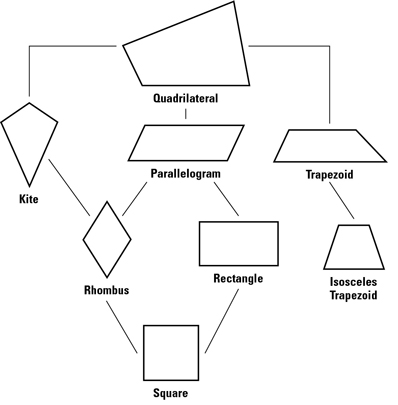
\includegraphics{4-Sided-Polygon}
%\end{figure}

\newpage
\begin{tcolorbox}
\begin{definition}
Quadrilateral 

A polygon is a quadrilateral if and only if it's a plane figure with four straight sides and angles. 
\end{definition}


\begin{definition}
Kite 

A quadrilateral is a kite if and only if it has the following properties: \\
1. Pairs of sides are congruent by definition \\
2. Only One pair of diagonally opposite angles is equal
3. Only one diagonal bisect the other angle \\
4. The diagonals are perpendicular bisectors of each other \\
\end{definition}


\begin{definition}
Parallelogram 

A quadrilateral is a parallelogram if and only if it has the following properties: \\
1. Parallel sides
2. Opposite angles are congruent 
3. Consecutive angles are supplementary
\end{definition}


\begin{definition}
Rhombus 

A parallelogram is a rhombus if and only if it has the following properties: \\
1. All the properties of a parallelogram \\
2. All sides are congruent by definition \\
3. The diagonals bisect the angles \\
4. The diagonals are perpendicular bisectors of each other \\
\end{definition}


\begin{definition}
Rectangle 

A parallelogram is a rectangle if and only if it has the following properties: \\
1. All the properties of a parallelogram \\
2. All angles are right angles by definition \\
3. The diagonals are congruent \\
\end{definition}


\begin{definition}
Square

A parallelogram is a square if and only if it has the following properties: \\
1. All the properties of a rhombus \\
2. All the properties of a rectangle apply \\
\end{definition}
\end{tcolorbox}

\newpage
\begin{definition}
4-Sided Polygon Theorems Examples \\

Examples of converse statements with necessary conditions that are not sufficient on the left and sufficient conditions that are not necessary on the right: \\

1. {\bf A Rectangle and Rhombus are necessary conditions of a plane figure to be a Square} is the converse ofdd the statement {\bf A Square is a sufficient condition for a plane figure to be a either a Rectangle or a Rhombus} \\


2. {\bf A Parallelogram is a necessary condition for a plane figure to be a a Rectangle} is the converse of the statement {\bf A Rectangle is a sufficient condition for a plane figure to be a Parallelogram}\\

3. {\bf A Kite or a Parallelogram is a necessary condition for a plane figure to be Rhombus} is the converse of the statement {\bf A Rhombus is a sufficient condition for a plane figure to be either a Kite or Parallelogram}\\

4. {\bf A Quadrilateral is a necessary condition for a plane figure to be a Kite} is the converse of the statement {\bf A Kite is a sufficient condition for a plane figure to to be a Quadrilateral} \\

5. {\bf A Quadrilateral is a necessary condition for a plane figure to be a Parallelogram} is the converse of the statement {\bf A Parallelogram is a sufficient condition for a plane figure to be Quadrilateral} \\
\end{definition}

\newpage
\begin{definition}
Conjunctive and Disjunctive Statements involving Necessary and Sufficient Conditions \\

The relationship between the two conditions must be exactly one of the following four possibilities: \\
1. $nec \wedge suf$ CASE: {\bf $[P$ necessary $Q] \wedge [P$ sufficient $Q]$} \\
\begin{center}
\begin{tabular}{|c|c|c|c|c|}
\hline 
P & Q & P nec Q & P suf Q & $[P$ nec $Q] \wedge [P$ suf $Q]$  \\ 
\hline 
T & T & T & T & T\\ 
\hline 
T & F & T & F & F\\ 
\hline 
F & T & F & T & F\\ 
\hline 
F & F & T & T & T\\ 
\hline 
\end{tabular} 
\end{center}

2. $nec \vee suf$ CASE: {\bf $[P$ necessary $Q] \vee [P$ sufficient $Q]$} \\
\begin{center}
\begin{tabular}{|c|c|c|c|c|}
\hline 
P & Q & P nec Q & P suf Q & $[P$ nec $Q] \wedge [P$ suf $Q]$  \\ 
\hline 
T & T & T & T & T\\ 
\hline 
T & F & T & F & T\\ 
\hline 
F & T & F & T & T\\ 
\hline 
F & F & T & T & T\\ 
\hline 
\end{tabular} 
\end{center}

3. $\neg nec \wedge suf$ CASE: {\bf $\neg[P$ necessary $Q] \wedge [P$ sufficient $Q]$} \\
\begin{center}
\begin{tabular}{|c|c|c|c|c|}
\hline 
P & Q & P nec Q & P suf Q & $\neg[P$ nec $Q] \wedge [P$ suf $Q]$  \\ 
\hline 
T & T & T & T & F\\ 
\hline 
T & F & T & F & F\\ 
\hline 
F & T & F & T & T\\ 
\hline 
F & F & T & T & F\\ 
\hline 
\end{tabular} 
\end{center}


4. $nec \wedge \neg suf$ CASE: {\bf $[P$ necessary $Q] \wedge \neg[P$ sufficient $Q]$} \\
\begin{center}
\begin{tabular}{|c|c|c|c|c|}
\hline 
P & Q & P nec Q & P suf Q & $\neg[P$ nec $Q] \wedge \neg[P$ suf $Q]$  \\ 
\hline 
T & T & T & T & F\\ 
\hline 
T & F & T & F & T\\ 
\hline 
F & T & F & T & F\\ 
\hline 
F & F & T & T & F\\ 
\hline 
\end{tabular} 
\end{center}

5. $\neg nec \vee suf$ CASE: {\bf $\neg[P$ necessary $Q] \vee [P$ sufficient $Q]$} \\
\begin{center}
\begin{tabular}{|c|c|c|c|c|}
\hline 
P & Q & P nec Q & P suf Q & $\neg[P$ nec $Q] \vee [P$ suf $Q]$  \\ 
\hline 
T & T & T & T & T\\ 
\hline 
T & F & T & F & F\\ 
\hline 
F & T & F & T & T\\ 
\hline 
F & F & T & T & T\\ 
\hline 
\end{tabular} 
\end{center}


6. $nec \vee \neg suf$ CASE: {\bf $[P$ necessary $Q] \vee \neg[P$ sufficient $Q]$} \\
\begin{center}
\begin{tabular}{|c|c|c|c|c|}
\hline 
P & Q & P nec Q & P suf Q & $[P$ nec $Q] \vee \neg[P$ suf $Q]$  \\ 
\hline 
T & T & T & T & T\\ 
\hline 
T & F & T & F & T\\ 
\hline 
F & T & F & T & F\\ 
\hline 
F & F & T & T & T\\ 
\hline 
\end{tabular} 
\end{center}


7. $\neg(nec \wedge suf)$ CASE: {\bf $\neg([P$ necessary $Q] \wedge [P$ sufficient $Q])$} \\
\begin{center}
\begin{tabular}{|c|c|c|c|c|}
\hline 
P & Q & P nec Q & P suf Q & $\neg[P$ nec $Q] \vee \neg[P$ suf $Q]$  \\ 
\hline 
T & T & T & T & F\\ 
\hline 
T & F & T & F & T\\ 
\hline 
F & T & F & T & T\\ 
\hline 
F & F & T & T & F\\ 
\hline 
\end{tabular} 
\end{center}

8. $\neg(nec \vee suf)$ CASE: {\bf $\neg([P$ necessary $Q] \vee [P$ sufficient $Q])$} \\
\begin{center}
\begin{tabular}{|c|c|c|c|c|}
\hline 
P & Q & P nec Q & P suf Q & $\neg[P$ nec $Q] \wedge \neg[P$ suf $Q]$  \\ 
\hline 
T & T & T & T & F\\ 
\hline 
T & F & T & F & F\\ 
\hline 
F & T & F & T & F\\ 
\hline 
F & F & T & T & F\\ 
\hline 
\end{tabular} 
\end{center} 
\end{definition}

\begin{definition}
Synonyms of Implication

\begin{center}
\begin{tabular}{|c|c|}
\hline 
FORM 1 & FORM 2 \\ 
\hline 
If $P$, then $Q$ & $P$ if $Q$ \\ 
\hline 
$P$ implies $Q$ & $Q$ is necessary for $P$ \\ 
\hline 
$P$ only if $Q$ & $Q$ is true whenever $P$ is true \\ 
\hline 
$P$ is sufficient for $Q$ & • \\ 
\hline 
Whenever $P$ is true, Q is true & • \\ 
\hline 
$Q$ if $P$ & • \\ 
\hline 
\end{tabular} 
\end{center}
\end{definition}



\newpage
\subsection{Logically Equivalent Statements}
\begin{definition}
Logically Equivalent Statement \\

Two expressions are logically equivalent provided that they have the same truth value for all possible combinations of truth values for all variables appearing in the two expressions. In this case, we write $X \equiv Y$ and say that $X$ is logically equivalent to $Y$ \\
\end{definition}

\begin{tcolorbox}
\begin{theorem}
Logical Equivalent Biconditional Statement \\
For the statements $P$, $Q$, and $R$: \\
\begin{tabular}{|c|c|c|}
\hline 
Num & Theorem Name & Logically Equivalent Statements \\ 
\hline 
1 & De Morgan Law & $\neg(P \wedge Q) \equiv \neg P \vee \neg Q$ \\ 
\hline 
2 & De Morgan Law & $\neg(P \vee Q) \equiv \neg P \wedge \neg Q$ \\ 
\hline 
3 & Conditional Statements  & $P \to Q \equiv \neg P \vee Q$ \\ 
\hline 
4 & Conditional Statements & $\neg (P \to Q) \equiv P \wedge \neg Q$ \\ 
\hline 
5 & Conditional Statements & $P \to Q \equiv \neg Q \to \neg P$ \\ 
\hline 
6 & Biconditional Statements & $P \leftrightarrow Q \equiv (P \to Q) \wedge (Q \to P)$ \\ 
\hline 
7 & Double Negation & $\neg(\neg P) \equiv P$ \\ 
\hline 
8 & Distribution Law & $P \vee (Q \wedge R) \equiv (P \vee Q) \wedge (P \vee R)$ \\ 
\hline 
9 & Distribution Law & $P \wedge (Q \vee R) \equiv (P \wedge Q) \vee (P \wedge R)$ \\ 
\hline 
10 & Conditional with Disjunction & $P \to (Q \vee R) \equiv (P \wedge \neg Q) \to R$ \\ 
\hline 
10 & Conditional with Disjunction & $(P \vee Q) \to R \equiv (P \to R) \wedge (Q \to R)$ \\ 
\hline 
\end{tabular} 
\end{theorem}
\end{tcolorbox}





\newpage
\subsection{Quantifiers and Negation}

\begin{definition}
Universal Quantifier \\

The phrase "for every" (or its equivalent) is called a {\bf Universal Quanfifier}. The symbols $\forall$ is used to denote a Universal Quantifier. \\
Using this notation, the statement, "For each real number $x$, $x^2 > 0$ could be written in symbolic form as $(\forall x \in \mathbb{R})(x^2 > 0)$.  

\end{definition} 


\begin{definition}
Existential Quantifiers \\

The phrase "there exists" (or its equivalents) is called an {\bf Existential Quantifier}. The symbol $\exists$ is used to denote an existential quantifier. \\
Using this notation, the statement, "There exists an integer $x$ such that $3x - 2 = 0$" could be written in symbolic form as $(\exists x \in \mathbb{Z})(3x - 2 = 0)$
\end{definition} 


\begin{definition}
Properties of Quantifiers \\

\begin{center}
	\begin{tabular}{|c|c|c|}
		\hline 
		{\bf A Statement Involving} & {\bf Often has the form} & {\bf Statement is true provided that} \\ 
		\hline 
		$(\forall x, P(x))$ & For every $x$, $P(x)$ & Every value of $x$, $P(x)$ true \\ 
		\hline 
		$(\exists x, P(x))$ & There exists an $x$, $P(x)$ & At least one value of $x$, $P(x)$ true \\  
		\hline 
	\end{tabular} 
\end{center}
\end{definition}



\begin{example}
Consider the following statements written in symbolic form: $(\forall \in \mathbb{Z})(x \text{ is a multiple of }2)$. \\
A. As an English sentence: For all integers $x$, $x$ is a multiple of $2$ \\
B. Truth Value: This statement is false because all integers cannot be written in form $2a$ \\
C. Negation: There exists some integer $x$ such that $x$ is not a multiple of $2$ \\
E. Negation: $(\exists \in \mathbb{Z})(x \text{ is not a multiple of }2)$ \\
\end{example}


\begin{example}
Consider the following statements written in symbolic form: $(\exists \in \mathbb{Z})(x^3 > 2)$. \\
A. As an English sentence: There exist some integer $x$ such that $x^3 > 0$
B. Truth Value: This statement is true becuase at least one integer meets the criteria of the predicate \\
C. Negation: For all integers $x$, $x^3 \leqq 0$ \\
E. Negation: $(\forall \in \mathbb{Z})(x^3 \leqq 0)$ \\
\end{example}


\begin{definition}
Negation of Quantified Statements \\

For any open sentence $P(x)$, \[ \neg(\forall x \in U)[P(x)] \equiv (\exists x \in U)[\neg P(x)]\]  and \[ \neg(\exists x \in U)[P(x)] \equiv (\forall x \in U)[\neg P(x)]\]
\end{definition}


\begin{example}
Consider $(\forall x \in \mathbb{R})(x^3 \geqq x^2)$ \\

We can write this statement  as an English sentence in several ways. The following are two different ways to do so: \\
1. For each real number $x$, $x^3 \geqq x^2$ \\
2. If $x$ is a real number, then $x^3$ is greater than or equal to $x^2$ \\
We can write the negation of the statement as \[ \neg (\forall x \in \mathbb{R})(x^3 \geqq x^2) \equiv (\exists x \in \mathbb{R}) \neg (x^3 \geqq x^2) \equiv (\exists x \in \mathbb{R})(x^3 < x^2) \]

Similarly, we can write the negation as an English sentence is several ways. The following are two differenct ways to do so: \\
1. These exists a real number $x$ such that $x^3 < x^2$ \\
2. There exists an $x$ such that $x$ is a real number and $x^3 < x^2$
\end{example}


\begin{definition}
Counterexample \\

Suppose $(\forall x \in \mathbb{R})(x^3 \geqq x^2)$, The real number $x = -1$ can use to show that this statement is false. This is called a {\bf counterexample} to the statement. \\
In general, a {\bf counterexample} to a statement of the form $(\forall)[P(x)]$ is an object $a$ in the universal set U for which $P(a)$ is false. It is an example that proves that $(\forall)[P(x)]$ is a false statement, and hence its negation, $(\exists x)[\neg P(x)]$, is a true statement
\end{definition}

\begin{definition}
Negation of Conditional Statements \\

The negation of the conditional statement "If $P$ then $Q$" is the statement "$P$ and not $Q$". Symbolically, this can be written as follows: \[ \neg (P \to Q) \equiv P \wedge \neg Q \]. So when we specifically include the universal quantifier, the symbolic form of the negation of a conditional statement is \[ \neg(\forall x \in U)[P(x) \to Q(x)] \equiv (\exists x \in U)\neg[P(x) \to Q(x)] \equiv (\exists x \in U)[P(x) \wedge \neg Q(x)] \]. That is \[ \neg(\forall x \in U)[P(x) \to Q(x)] \equiv (\exists x \in U)[P(x) \wedge \neg Q(x)] \]
\end{definition}


\begin{definition}
Quantifiers in Definitions \\

Definitions of terms in mathematics often involve quantifiers even though the quantifer symbolism might not be present. For instance, let's examine the definition of square numbers (perfect squares), 
	\begin{center}
	\bf A natural number $n$ is a perfect square provided that there exists a natural number $k$ such that $n = k^2$
	\end{center}
This definition of perfect squares can be represented as a quantified definition as follows:
	\begin{center}
	\bf A natural number $n$ is a perfect square provided $(\exists k \in \mathbb{N})(n = k^2)$
	\end{center}
On the other hand,, when we say that a natural number $n$ is not a perfect, we need to negate the condition that there exists a natural number $k$ such that $n = k^2$. We use the symbolic form to do this. 
	\begin{center}
	$\neg(\exists k \in \mathbb{N})(n = k^2) \equiv (\forall k \in \mathbb{N})\neg(n = k^2) \equiv (\forall k \in \mathbb{N})(n \neq k^2)$
	\end{center}
This negated definition can easily be translated into an English sentence, 
	\begin{center}
	\bf A natural number $n$ is not a perfect square provided that for every natural number $k$, $n \neq k^2$
	\end{center}
\end{definition}


\begin{definition}
Compound Quantified Statements \\

When a predicate contain more than variable, each variable must be quantified to create a statement. For example, assume  the universal set is the set of integers, $\mathbb{Z}$, and let $P(x,y)$ be the predicate $x + y = 0$. We can create a statement from this predicate in several ways: \\
1. $(\forall x \in \mathbb{Z})(\forall y \in \mathbb{Z})(x + y = 0)$ is read "For all integers $x$ and $y$, $x + y = 0$" \\
2. $(\forall x \in \mathbb{Z})(\exists y \in \mathbb{Z})(x + y = 0)$ is read "For every integer $x$, there exists an integer $y$ such that $x + y = 0$"\\
3. $(\exists x \in \mathbb{Z})(\forall y \in \mathbb{Z})(x + y = 0)$ is read "There exists and integer $x$ such that for every integer $y$, $x + y = 0$"\\
4. $(\exists x \in \mathbb{Z})(\exists y \in \mathbb{Z})(x + y = 0)$ is read "There exists integers $x$ and $y$ such that $x + y = 0$" \\
\end{definition}


\begin{definition}
Negation of Compound Quantified Statements \\

When we negate a statement with more than one quantifier, we consider each quantifer in turn and apply the negation of quantified statement theorem. As an example, we will negate the statement $(\exists x \in \mathbb{Z})(\forall y \in \mathbb{Z})(x + y = 0)$. 
Firstly, we will treat this as a statement in the following form $(\exists x \in \mathbb{Z})[P(x)]$, where $P(x)$ is the predicate $(\forall y \in \mathbb{Z})(x + y = 0)$. Using the negation of quantified statements theorem, we have: \[ \neg (\exists x \in \mathbb{Z})[P(x) \equiv (\forall x \in \mathbb{Z})[\neg P(x)] \] Now let's  examine the negation of the predicate $\neg P(x)$. Again, using the negation of quantified statements theorem, we have: 
	\begin{eqnarray}
		\neg P(x) & = & \neg (\forall y \in \mathbb{Z})(x + y = 0) \nonumber \\
		& = & (\exists y \in \mathbb{Z})\neg (x + y = 0) \nonumber \\
		& = & (\exists y \in \mathbb{Z})(x + y \neq 0) \nonumber \\
	\end{eqnarray}
Combining these two results, we obtain \[ \neg (\exists x \in \mathbb{Z})(\forall y \in \mathbb{Z})(x + y = 0) \equiv (\forall x \in \mathbb{Z})(\exists y \in \mathbb{Z})(x + y \neq 0) \].

\end{definition}





\newpage
\section{Proof Writing Techniques}
\subsection{s.3.1. Proof Technique: Trivial and Vacuous Proofs}
\subsubsection*{s.3.1. Proof Technique: Trivial Proof}
\begin{definition}
Trivial Proof

When the quantified statement $\forall x \in S$, $P(x) \to Q(x)$ is expressed as a result or theorem, we often write such a statement as: 
	\begin{center}
		For $x \in S$, if $P(x)$, then $Q(x)$ 
	\end{center}
or as 
	\begin{center}
		Let $x \in S$, if $P(x)$, then $Q(x)$
	\end{center}
Thus, the proposition $(\forall x \in S)[P(x) \to Q(x)]$ is true if $P(x) \to Q(x)$ is a true statement for  each $x \in S$, while the proposition $(\forall x \in S)[P(x) \to Q(x)]$ is false if $P(x) \to Q(x)$ is false for at least one element $x \in S$. In the proposition $(\forall x \in S)[P(x) \to Q(x)]$, if $Q(x)$ us true for all $x \in S$ if $P(x)$ is false for all $x \in S$, then determining the truth or falseness of the proposition $(\forall x \in S)[P(x) \to Q(x)]$ becomes considerably easier. \\
Indeed, if it can be shown that $Q(x)$ is true for all $x \in S$ (regardless of the truth value of $P(x)$ ), then, according to the truth table for the implication, is true. This constitutes a proof of the proposition $(\forall x \in S)[P(x) \to Q(x)]$ and is called a {\bf Trivial Proof}. For instance: 


\begin{tcolorbox}
	\begin{theorem}
		For all real numbers $x$. If $x>0$, then $x^2 + 5 > 0$
	\end{theorem}
\end{tcolorbox}

\begin{proof}
We assume $x$ is real number and that $x>0$, we will show via a trivial proof that $x^2 + 5 > 0$. Since $x^2 \geqq 0$ for all real numbers $x$, it follows that:
	\begin{equation}
		(x^2 + 5) > x^2 \geqq 0 \nonumber 
	\end{equation}
Hence, $x^2 + 5 \geqq 0$. Consequently, if $x>0$, then $x^2 + 5 > 0$
\end{proof}
\end{definition}





\newpage
\subsubsection*{s.3.1. Proof Technique: Vacuous Proof}
\begin{definition}
Vacuous Proof

Let $P(x)$ and $Q(x)$ be open sentences over a domain $S$. the $\forall x \in S$, $P(x) \to Q(x)$ is a true statement if it can be shown that $P(x)$ is false for all $x \in S$ (regardless of the trith value $Q(x)$), according to the truth table for implications. Such a proof is called a {\bf Vacuous Proof} of $\forall x \in S$, $P(x) \to Q(x)$. For instance, 

\begin{tcolorbox}
	\begin{theorem}
		For all real numbers $x$. If $x^2 + 1 < 0$, then $x^5 \geqq 4$
	\end{theorem}
\end{tcolorbox}

\begin{proof}
We assume $x$ is real number and that $x^2 + 1 < 0$, we will show via a vacuous proof that $x^5 > 4$. Observe that 
	\begin{equation}
		(x^2 + 1) > x^2 \geqq 0 \nonumber 
	\end{equation}

Hence, $x^2 + 1 < 0$ is false for all value of the real number $x$. Consequently, if $x^2 + 1 < 0$, then $x^5 \geqq 4$
\end{proof}

\end{definition}



\newpage
\subsection{s.3.1. Proof Examples: Trivial and Vacuous Proofs}

\begin{example}
Let $x \in \mathbb{R}$. Prove that $0<x<1$, then $x^2-2x + 2 \neq 0$

\begin{tcolorbox}
	\begin{theorem}
		If $0<x<1$, then $x^2-2x + 2 \neq 0$
	\end{theorem}
\end{tcolorbox}

\begin{proof}
We assume $x$ is real number and that $0<x<1$, we will show via a trivial proof that $x^2 -2x + 2 \neg 0$. By factoring the consequent, 
	\begin{equation}
		x^2 - 2x + 2 = (x-2)(x-1)  \nonumber 
	\end{equation}
Since the solution set of the consequent is $(\forall x \in \mathbb{R})[ 1, 2]$. Consequently, If $0<x<1$, then $x^2-2x + 2 \neg 0$

\end{proof}
\end{example}


\begin{example}
Let $n \in \mathbb{N}$. Prove that $|n-1|+|n+1| \leqq 1$, then $|n^2-1| \leqq 4$

\begin{tcolorbox}
	\begin{theorem}
		If $|n-1|+|n+1| \leqq 1$, then $|n^2-1| \leqq 4$
	\end{theorem}
\end{tcolorbox}

\begin{proof}
We assume $n$ is natural number and that $|n-1|+|n+1| \leqq 1$, we will show via a trivial proof that $|n^2-1| \leqq 4$. By the definition of absolute value function $|n^2-1| \leqq 4$. We can rewrite the consequent as follows: 
	\begin{equation}
		|n^2-1| \leqq 4 \equiv \left\{ 
			\begin{array}{rcl}\
				(n-1)(n+1)\leqq 4 & \mbox{for} & n \leqq 2 \\ 
				(1-n)(n+1) > 4 & \mbox{for} & n > 2 
			\end{array} \right.  \nonumber 
	\end{equation}
Since the consequent holds trivially true for all values of the natural number $n$. We conclude that if $|n-1|+|n+1| \leqq 1$, then $|n^2-1| \leqq 4$

\end{proof}
\end{example}


\begin{example}
Let $r \in \mathbb{Q}^+$. Prove that $\frac{r^2 + 1}{r} \leqq 1$, then $\frac{r^2 + 2}{r} \leqq 2$

\begin{tcolorbox}
	\begin{theorem}
		If $\frac{r^2 + 1}{r} \leqq 1$, then $\frac{r^2 + 2}{r} \leqq 2$
	\end{theorem}
\end{tcolorbox}

\begin{proof}
We assume $r$ is a positive rational number where $\frac{r^2 + 1}{r} \leqq 1$, we will show via a vacuous proof that $\frac{r^2 + 2}{r} \leqq 2$. we will proceed by demonstrating that the antecedent is a false proposition by showing that the negation of the antecedent is true statement. Since the negation of the antecedent is that the exists a positive rational number $r$ such that $\frac{r^2 + 1}{r} > 1$. \\ 
Suppose that $r = \frac{2}{3}$, it follows that; 

	\begin{equation}
		\frac{r^2 + 1}{r}>\frac{(\frac{2}{3})^2+1}{\frac{2}{3}} = 2\frac{1}{6}>1 \nonumber 
	\end{equation}

Since negation of the antecedent is a true proposition, $\frac{r^2 + 1}{r} \leqq 1$ is vacuously false for all values of the positive rational number $r$. Consequently, if $\frac{r^2 + 1}{r} \leqq 1$, then $\frac{r^2 + 2}{r} \leqq 2$.
\end{proof}
\end{example}


\begin{example}
Let $x \in \mathbb{R}$. Prove that $x^3 -5x - 1 \geqq 0$, then $(x-1)(x-3)\geqq -2$

\begin{tcolorbox}
	\begin{theorem}
		If $x^3 -5x - 1 \geqq 0$, then $(x-1)(x-3)\geqq -2$
	\end{theorem}
\end{tcolorbox}

\begin{proof}
We assume $x$ is real number with $x^3 -5x - 1 \geqq 0$, and we will show via a trivial proof that $(x-1)(x-3)\geqq -2$. Using algebra, we can rewrite the consequent in the form: 
\begin{alignat*}{2}
 	(x-1)(x-3) 			& \geqq -2 & \\
 	x^2 -4x + 3  		& \geqq -2\\
 	(x^2 -4x + 4) - 1 	& \geqq -2& \\
 	(x-2)^2 -1			& \geqq -2& \\
 	(x-2)^2				& \geqq -1& \\
\end{alignat*}
Since, 
	\begin{equation}
		(x-1)(x-3) \geqq -2 \equiv (x-2)^2 \geqq -1  \nonumber 
	\end{equation}
we conclude that the consequent is trivally true. In order words, if $x^3 -5x - 1 \geqq 0$, then $(x-1)(x-3)\geqq -2$. 
\end{proof}
\end{example}



\begin{example}
Let $n \in \mathbb{N}$. Prove that $n + \frac{1}{n} < 2$, then $n^2 + \frac{1}{n^2} < 4$

\begin{tcolorbox}
	\begin{theorem}
		If $n + \frac{1}{n} < 2$, then $n^2 + \frac{1}{n^2} < 4$
	\end{theorem}
\end{tcolorbox}

\begin{proof}
We assume $n$ is a natural number where $n + \frac{1}{n} < 2$, and we will show via a vacuous proof that $n^2 + \frac{1}{n^2} < 4$. We will proceed by demonstrating that the antecedent is a false proposition by showing that the negation of the antecedent is true statement. Since the negation of the antecedent is that the exists a natural number $n$ such that $n + \frac{1}{n} \geqq 2$. \\ 
Suppose that $n = 2$, it follows that; 

	\begin{equation}
		n + \frac{1}{n} \geqq 2 + \frac{1}{2} \geqq 2\frac{1}{2} \geqq 2 \nonumber 
	\end{equation}

Since negation of the antecedent is a true proposition, $n + \frac{1}{n} < 2$ is vacuously false for all values of the natural number $n$. Consequently, if $n + \frac{1}{n} < 2$, then $n^2 + \frac{1}{n^2} < 4$
\end{proof}
\end{example}








\newpage
\subsection{s.3.1. Proof Technique: Counterexample}

\begin{example}
Proof by Counterexample

\begin{tcolorbox}
	\begin{conjecture}
		For each integer $n$, if $5$ divides $(n^2 + 1 )$, then $5$ divides $(n + 1)$
	\end{conjecture}
\end{tcolorbox}

The integer $n = 4$ is a counterexample that proves this conjecture is false. Notice that when $n=4$, $n^2 - 1 = 15$ and $5$ divides $15$. Hence the hypothesis of the conjecture is true in this case. In addition, $n - 1 = 3$ and $5$ does not divide $3$ and so the conclusion is false in this case. Since this is an example where the hypothesis is true and the conlcusion is false, the conjecture is false. 
\end{example}





\newpage
\subsection{s.3.1. Proof Technique: Biconditional}
When proving a biconditional statment using the logical equivalency $P \leftrightarrow Q \equiv (P \to Q) \wedge (Q \to P)$, we actually need to prove two conditional statements. The proof of each conditional statement can be considered as one of two parts of the proof of the biconditional statement. Make sure that the start and end of each parts is indicated clearly. This is clearly indicated in the biconditional proof examples below: 

\begin{example}
Let $x$ be a real number such that the real number $x$ equals $2$ if and only if $x^3 - 2x^2 + x = 2$

\begin{tcolorbox}
	\begin{theorem}
		The real number $x = 2$ if and only if $x^3 - 2x^2 + x = 2 $
	\end{theorem}
\end{tcolorbox}

\begin{proof}
We will prove this biconditional statement by proving the following two conditional statements: \\
1. For each real number $x$, if $x$ equals $2$, then $x^3 -2x^2 + x = 2$ \\
2. For each real number $x$, if $x^3 -2x^2 + x = 2$, then $x$ equals $2$ \\

For the forward direction, we assume $x$ is a real number such that $x = 2$. And, we will prove via direct proof that $x^3 -2x^2 + x = 2$. We will proceed by substituting $x = 2$ into the expression $x^3 -2x^2 + x = 2$, this gives:
	\begin{eqnarray*}
		2 & = & (2)^3 -2(2)^2 + (2) + 2 \nonumber \\
		& = & 8 - 8 + 2 \nonumber \\
		& = & 2 \nonumber \\
	\end{eqnarray*}
Since the expression becomes $2 = 2$ after substituting $x = 2$, we conclude that if $x$ equals $2$, then $x^3 -2x^2 + x = 2$ holds. This completes the proof of the forward direction. \\
For the backwards direction, we assume that $x$ is a real number such that if $x$ equals $2$, then $x^3 -2x^2 + x = 2$. And we will show via direct proof that $x = 2$. Factoring the expression $x^3 -2x^2 + x = 2$ yields: 
	\begin{eqnarray*}
		0 & = & x^3 -2x^2 + x - 2 \nonumber \\
		& = & x^2(x - 2) + (x - 2) \nonumber \\
		& = & (x - 2)(x^2 + 1) \nonumber \\
	\end{eqnarray*}
Now, in the real numbers, if a product of two factors is equal to zero, then one of the factors must be zero. So the last equation implies that $ (x = 2) \vee (x^2 = 1)$. Since $x^2 = 1$ has no real solution, we conclude that $x = 2$. This completes the backwards direction  proof. \\
Since, we have now proven both the directions of the biconditional, we have proven that the real number $x = 2$ if and only if $x^3 - 2x^2 + x = 2 $
\end{proof}

\end{example}




\newpage
\subsection{s.3.1. Proof Technique: Contrapositive}
One of the most useful logical equivalencies is a conditional statement $P \to Q$ is logically equivalent to its contrapositive $\neg Q \to \neg P$. This means that if we prove the contrapositve of the conditional statement, then we have proven the conditional statement. The following are some important points to remember: \\
1. A conditional statement is logically equivlent to its contrapositive \\
2. Use a direct prove to prove that $\neg Q \to \neg P$ is true \\
3. CAUTION: One difficulty with this tyoe of proof is in the formation of correct negations. (We need to be very careful doing this.) \\
4. We might consider using a proof by contraposive when the statement $P$ and $Q$ are stated as negations. \\ 


\begin{example}
If $n^2$ is an odd integer, then $n$ is an odd integer. \\

\begin{tcolorbox}
	\begin{theorem}
	\label{the}		
		If $n^2$ is an odd integer, then $n$ is an odd integer
	\end{theorem}
\end{tcolorbox}

\begin{proof}
We will prove this result by proving the contrapositve of this theorem which is
	\begin{center}
		If $n$ is an even integer, then $n^2$ is even integer
	\end{center}

We assume that $n$ is an even integer, and we will show that $n^2$ is even. Using the definitions of even integers, we see that $n = 2a$ for some integer $a$. Expressing $n^2$ in terms of $n = 2a$, using algebra we get
	\begin{eqnarray*}
		n^2 & = & (2a)^2  \nonumber \\ 
		& = & 2(2a^2) \nonumber \\
		& = & 2q \nonumber \\
	\end{eqnarray*}
Since $a$ is an integer closed under multiplication and addition, we conclude that $q$ is an integer. Such that $n^2 = 2q$ for some integer $q$, hence, $n^2$ is an even integer. We have thus proved the contrapostive of the theorem, and consequently, we have prove that if $n^2$ is an odd integer, then $n$ is an even integer. \\
\end{proof}
\end{example}



\subsubsection{Proofs by Contradiction Repository}
begin{example}
Let $x$ be an integer. If $5x - 7$ is an even integer, then $x$ is an odd integer. \\

\begin{tcolorbox}
	\begin{theorem}
	\label{the}		
		If $5x - 7$ is an even integer, then $x$ is an odd integer
	\end{theorem}
\end{tcolorbox}

\begin{proof}
We will prove this result by proving the contrapositve of this Theorem which is
	\begin{center}
		If $x$ is an even integer, then $5x - 7$ is an odd integer
	\end{center}

We assume that $x$ is an even integer, and we will show that $5x - 7$ is odd. Using the definitions of even integers, we see that $x = 2a$ for some integer $a$. Expressing $5x - 7$ in terms of $x = 2a$, using algebra we get
	\begin{eqnarray*}
		5x - 7 & = & 5(2a) - 7  \nonumber \\
		& = & 10a - 8 + 1 \nonumber \\
		& = & 2(5a - 4) + 1 \nonumber \\
		& = & 2q + 1 \nonumber \\
	\end{eqnarray*}
Since $5a - 4$ is an integer closed under multiplication and addition, we conclude that $q$ is an integer. Such that $5x - 7 = 2q + 1$ for some integer $q$, hence, $5x - 7$ is an odd integer. We have thus proved the contrapostive of the theorem, and consequently, we have prove that if $5x - 7$ is an even integer, then $x$ is an odd integer. \\
\end{proof}


















\begin{example}
Let $n \in \mathbb{Z}$. If $n^2 \neq n (\text{mod 3})$, then $n \neq 0 (\text{mod 3})$ and $n \neq 1 (\text{mod 3})$

\begin{tcolorbox}
	\begin{theorem}
	\label{the3}
		If $n^2 \neq n (\text{mod 3})$, then $n \neq 0 (\text{mod 3})$ and $n \neq 1 (\text{mod 3})$
	\end{theorem}
\end{tcolorbox}

We will prove this result by proving the contrapositve of Theorem \ref{the3} which is
	\begin{center}
		If $n = 0 (\text{mod 3})$ or $n = 1 (\text{mod 3})$, then $n^2 = n (\text{mod 3})$
	\end{center}
PROOF REQUIRED

\end{example}




\newpage
\subsection{s.3.1. Proof Technique: Existence Theorem I}

\begin{definition} 
Existence Theorem I

In an {\bf existence theorem} (sometimes called Constructive Proof or Existence Proof) the existence of an object (or objects) possessing some specified propery or properties is asserted. Typically then, an existence theorem is concerning an open sentence $P(x)$ over a domain $S$ can be expressed as a quantified statement
	\begin{center}
		$\{ \exists x \in S | P(x) \}$: There exists an $x \in S$ such that $P(x)$
	\end{center}
This proof technieque requires that we actually name, describe or explain how to construct some object in the universe that makes $P(x)$ true.
\end{definition}

\begin{example}
If $a$, $b$, and $c$ are real numbers with $a \neq 0$, then the linear equation $ax + b = c$ has exactly one one real number solution, which is $x = \frac{c-b}{a}$ \\

\begin{tcolorbox}
	\begin{theorem}
		The Linear equation $ax + b = c$ has exactly one one real number solution, which is $x = \frac{c-b}{a}$
	\end{theorem}
\end{tcolorbox}

\begin{proof}
We assume that $ax + b = c$ is a linear equation  with real number coefficients $a$, $b$, and $c$, such that $a \neq 0$; we will show via a constructive proof that the linear equation $ax + b = c$ has exactly one one real number solution, which is $x = \frac{c-b}{a}$. \\
We can solve the linear equation by adding $-b$ to both sides of the equation and then dividing both sides of the resulting equation by $a$, to obtain: 
	\begin{eqnarray*}
		x & = & \frac{c-b}{a}
	\end{eqnarray*}
This shows that if there is a solution, then it must be $x = \frac{c-b}{a}$. We also see that if $x = \frac{c-b}{a}$, then
	\begin{eqnarray*}
		ax + b & = & a(\frac{c-b}{a}) + b  \nonumber \\
		& = & (c-b) + b \nonumber \\
		& = & c \nonumber \\
	\end{eqnarray*}
Therefore, the linear equation $ax + b = c$ has exactly one real number solution and the solution is $x = \frac{c-b}{a}$. 
\end{proof}
\end{example}


\newpage
\subsection{s.3.1. Proof Technique: Existence Theorem II}

\begin{definition}
Existence Theorem II

Another type of proof that is often used to prove  an Existence Theorem is the {\bf Nonconstructive Proof}. For this type of proof, we make an argument that an object in the universal set that makes $P(x)$ true must exists but we never construct or name the object that makes $P(x)$ true. \\
For example, there are theorems in mathematics that tells us that every polynomial of odd degree with real coefficients has at least one real number in its solution set, but we don't know to find a real number solution for every such polynomial. 
\end{definition}

\begin{example}
The proof of the {\bf Intermediate Value Theorem} is an example of an Nonconstructive Proof.

\begin{tcolorbox}
	\begin{theorem}
		If $f$ is a continuous function on the closed interval $[a,b]$ and if $q$ is any real number strictly between $f(a)$ and $f(b)$, then there exists a number $c$ in the interval $(a,b)$ such that $f(c) = q$
	\end{theorem}
\end{tcolorbox}

\begin{proof}
Assume that $x$ is a real number. We will use the Intermediate Value Theorem to prove that the equation $x^3 - x + 1 = 0$ has a real number solution. \\
To investigate solutions of the equation $x^3 - x + 1 = 0$, we will use the function: 
	\begin{equation}
		f(x) = x^3 - x + 1 \nonumber
	\end{equation}
Notice that $f(-2) = - 5$ and that $f(0) = 1$. Since $f(-2) < 0$ and $f(0) > 0$, the Intermediate Value Theorem tells us that there is a real number $c$ in the interval $(-2, 0)$ such that $f(c) = 0$. This means that there exists a real number $c$ between $-2$ and $0$ such that: 
	\begin{equation}
		c^3 - c + 1 = 0 \nonumber
	\end{equation}
and hence $c$ is a real number solution of the equation $x^3 - x  + 1 = 0$. This proves that the equation $x^3 - x + 1 = 0$ has at least one real number solution. 
\end{proof}

NOTICE: this proof of the Intermediate Value Theorem does not tell us how to find the exact value of $c$. It does however, suggest a method for approximating the value of $c$. This can be done by finding a smaller and smaller interval $[a, b]$ such that $f(a)$ and $f(b)$ have opposite signs. 
\end{example}









\newpage
\subsection{s.3.1. Proof Technique: Contradiction}
Suppose, as usual, that we would like to show that a certain mathematical statement $R$ is true. If $R$ is expressed as the quantified statement: 
	\begin{center}
 		$\forall x \in S$, $P(x) \to Q(x)$
	\end{center}	  
Then we already have two possible proof techniques to prove such as statement: a direct proof and a proof by contrapositive. We now introduce a third proof technique that can be used to establish the truth of $R$, regardless of whether $R$ is expressed in term of an implication. \\ 

Suppose we assume $R$ is an false statement, from this assumption, we are able to arrive at or deduce a statement that contradicts some assumption we made in the proof or some known fact. (The known fact might be a definition, an axiom, or a previously proven theorem). If we denote this assumption or known fact by $P$, then what we have deduced is $\neg P$ and have thus produced the contridiction $C:P \wedge \neg P$. We  have therefore established the truth of the implication: 
	\begin{center}
		$\neg R \to C$
	\end{center}	 
However, because $\neg R \to C$ is true $C$ is false, it logically follows that $\neg R$ is false and so $R$ is true, as desired. This technique is called {\bf Proof by Contradiction}.\\

If $R$ is the quantified statement $\forall x \in S$, $P(x) \to Q(x)$, then a proof by contridiction of this statement consists of verifying the implication:
	\begin{center}
		$\neg [\forall x \in S$, $P(x) \to Q(x)] \to C$
	\end{center}
For some contradictory mathematical statement $C$. However, since  

	\begin{alignat*}{2}
 		\neg [\forall x \in S, P(x) \to Q(x)]	& \equiv \exists x \in S, \neg [P(x) \to Q(x)] & \\
 		& \equiv \exists x \in S,P(x) \wedge \neg Q(x) & \\	
	\end{alignat*} 
it follows that a proof by contridiction of $\forall x \in S, P(x) \to Q(x)$ would begin by assuming the \ of some element $x \in S$ such that $P(x)$ is true and $Q(x)$ is false.\\
{\bf That is, a proof by contradiction begins by assuming the existence of a counterexample of this quantified statement $\forall x \in S, P(x) \to Q(x)$ exists.} 


\newpage
\subsection*{Proof by Contradiction Repository}
\begin{example}
For each real number $x$, if $0 < x < 1$, then $\frac{1}{x(1-x)} \geqq 4$

\begin{tcolorbox}
	\begin{theorem}
	\label{the2}		
		If $0 < x < 1$, then $\frac{1}{x(1-x)} \geqq 4$
	\end{theorem}
\end{tcolorbox}

\begin{proof}

We will prove this result by proving the negation of the proposition which is
	\begin{center}
		There exists some real number $x$ such that $0 < x < 1$ and $\frac{1}{x(1-x)} < 4$
	\end{center}

We assume that $x$ is a real number, where $0 < x < 1$. We note that since $0 < x < 1$, we conclude that $x > 0$ and $1-x > 0$ if we multiply both sides of the inequality $\frac{1}{x(1-x)} < 4$ by $x(1-x)$ we obtain: 
	\begin{center}
		$1 < 4x(1-x)$
	\end{center}
We can now use algebra to rewrite the last inequality as follows: 
	\begin{alignat*}{2}
		1 				&< 4x(1-x)& \\
		4x^2 - 4x + 1 	&< 0& \\
		(2x - 1)^2 		&< 0& \\
	\end{alignat*} 
However, $(2x - 1)$ is a real number and the last inequality say that a real number squared is less than zero. This is a contradiction since the square of any real number must be greater or equal to zero. Hence, the proposition cannot be false. Consequently, for each real number $x$, $0 < x < 1$, then $\frac{1}{x(1-x)} \geqq 4$

\end{proof}
\end{example}


\newpage
\begin{example}
For each real numbers $x$ and $y$, if $x$ is rational and $x \neq 0$ and $y$ is irrational, then $x \cdot y$ is irrational
\begin{tcolorbox}
	\begin{theorem}
	\label{the2}		
		If $x$ is rational and $x \neq 0$ and $y$ is irrational, then $x \cdot y$ is irrational
	\end{theorem}
\end{tcolorbox}

\begin{proof}

We will prove this result by proving the negation of the proposition which is
	\begin{center}
		There exists some real number $x$ and $y$ such that $x$ is rational, $x \neq 0$, $y$ is irrational and $x \cdot y$ rational
	\end{center}

We assume that $x$ and $y$ are real numbers such that $x$ is rational, $x \neg 0$, $y$ is irrational and $x \cdot y$ rational. Since $x \neg 0$, we can divide by $x$ and since the rational numbers are closed under division by nonzero rational numberes, we know that $\frac{1}{x} \in \mathbb{Q}$. We now know that $x \cdot y$ and $\frac{1}{x}$ are rational numbers and since the rational numbers are closed under multiplication, we conclude that: 
	\begin{equation}
		\frac{1}{x} \cdot (xy) \in \mathbb{Q}
	\end{equation}
However, $\frac{1}{x} \cdot (xy) = y$ and hence, $y$ must be rational number. Since a real number cannot be both rational and irrational, this is a contradiction to the assumption that $y$ is irrational. We have therefore proved that for all real numbers $x$ and $y$, if $x$ is rational and $x \neq 0$ and $y$ is irrational, then $x \cdot y$ is irrational

\end{proof}
\end{example}


\newpage
\begin{example}
There is not smallest positive real number
\begin{tcolorbox}
	\begin{theorem}
	\label{the2}		
		There is no smallest positive real number
	\end{theorem}
\end{tcolorbox}

\begin{proof}

We will prove this result by proving the negation of the proposition which is
	\begin{center}
		There exists a smallest positive real number
	\end{center}

We assume that $r$ is the smallest positive real number. Since $0 < \frac{r}{2} < r$, it follows that $\frac{r}{2}$ is a positive real number that is smaller than $r$. This however is a contradiction. We have therefore proved that there is no smallest positive real number. 

\end{proof}
\end{example}

\newpage
\begin{example}
No odd integer can be expressed as the sum of three even integers
\begin{tcolorbox}
	\begin{theorem}
	\label{the2}		
		No odd integer can be expressed as the sum of three even integers
	\end{theorem}
\end{tcolorbox}

\begin{proof}
    We will prove this result by proving the negation of the proposition which is
    	\begin{center}
    		There exists a odd integer which can be expressed as the sum of three even integers
    	\end{center}
    
    We assume that $x$, $y$, $z$, and $n$ are integers, such that $x$, $y$ and $z$ are even integers. We also assume that $n$ is an odd integer. We can express $n$ as the sum of three even integers $n = x + y + z$. By the definition of even integers, we let $x=2a$, $y=2b$ and $z=2c$, where $a$, $b$, and $c$ are integers. Now, substituting $x$, $y$ and $z$ into the equation $n = x + y + z$ yields
    		\begin{eqnarray*}
    			n & = & x + y + z \nonumber \\
    			& = & 2a + 2b + 2c \nonumber \\
    			& = & 2(a + b + c) \nonumber \\
    		\end{eqnarray*}
    Since $a + b + c$ are integers and integers are closed under addition. Then, $n=2k$ for some integer $k = a + b + c$. This is a contradiction. We have therefore proved that there is no odd integer can be expressed as the sum of three even integers.
\end{proof}
\end{example}


\newpage
\begin{example}
For all integers $a$ and $b$
\begin{tcolorbox}
	\begin{theorem}
	\label{the2}		
		If $a$ is an even integer and $b$ is an odd integer, then $4 \nmid (a^2 + b^2)$ 
	\end{theorem}
\end{tcolorbox}

\begin{proof}
    We will prove this result by proving the negation of the proposition which is
    	\begin{center}
    		There exists an even integer $a$ and an odd integer $b$, such that $4 | (a^2 + 2b^2)$
    	\end{center}
    
    Using the definition of odd and even integers, $a = 2x$ and $b = 2y + 1$, for some integer $x$ and $y$; using the divisibility property of integers, we see that $a^2 + b^2 = 4z$, for some integer $z$. Thus, substituting $a = 2x$ and $b = 2y + 1$ into $a^2 + b^2 = 4z$ yields: 
        \begin{align*}
            (2x)^2 + (2y + 1)^2 & = 4z \\
            4x^2 + 2(4y^2 + 4y + 1) & = 4z \\
            4x^2 + 8y^2 + 8y + 2 & = 4z \\
            2 & = 4z - 4x^2 - 8y^2 - 8y  \\
            2 & = 4(z - x^2 - 2y^2 - 2y) \\
        \end{align*}
    Since $z - x^2 - 2y^2 - 2y$ is an integer becuase integers are closed under addition and multiplication, such that $4 | 2$. By the divibility propery of integers, we have a contradition because $4 \nmid 2$. Hence the proposition is true. 
\end{proof}
\end{example}



\newpage
\begin{example}
Prove that the integer $100$ cannot be written as the sum of three integers, an odd number of which are odd. 
\begin{tcolorbox}
    \begin{theorem}
        The integer $100$ cannot be written as the sum of three integers, an odd number of which are odd 
    \end{theorem}
\end{tcolorbox}

\begin{proof}
    We assume that $a$, $b$, and $c$ are integers and will proceed by cases to prove the negation of the proposition that  
        \begin{center}
            For an odd number of odd integers $a$, $b$, and $c$,
                \begin{equation*}
                    100 = a + b + c
                \end{equation*}
        \end{center}
    \textit{Case 1: Exactly one of $a$, $b$ and $c$ is odd} \\
        We assume, without loss of generality, that $a$ is odd. By the definition of integer, $a = 2x + 1$, $b = 2y$, and $c = 2z$, for some integers $x$, $y$ and $z$. adding these integers, yield:
            \begin{align*}
                100 & = a + b + c \\
                100 & = (2x + 1) + 2y + 2z \\
                100 & = 2x + 2y + 2z + 1 \\
                100 & = 2(x + y + z) + 1 \\
            \end{align*}
        Since $x + y + z$ is an integer, we see that $2(x + y + z) + 1$ is odd integer and that $100$ is an even intger. Since odd integer is not equal to an even intger, we have a contradiction. Consequently, $100$ cannot be written as the sum of a odd and two even integers. \\
    
    \textit{Case 2: All of $a$, $b$ and $c$ are odd} \\
        Again, using the definition of integgers, $a = 2p + 1$, $b = 2q + 1$, and $c = 2r + 1$, for some integers $p$, $q$ and $r$; adding these integers, yield:
            \begin{align*}
                100 & = a + b + c \\
                100 & = (2p + 1) + (2q + 1) + (2r + 1) \\
                100 & = 2p + 2q + 2r + 2 + 1 \\
                100 & = 2(p + q + r + 1) + 1 \\
            \end{align*}
        Since $p + q + r + 1$ is an integer, we see that $2(p + q + r + 1) + 1$ is an odd integer and that $100$ is an even integer. Since integers cannot have dual parity, we have a contrdition. Consequently, $100$ cannot be written as the sum of three odd integers. \\
        
    Because we have proven both conditional statements, we have proven that the integer $100$ cannot be written as the sum of three integers, an odd number of which are odd. 
\end{proof}
\end{example}

\newpage
\begin{example}
Prove that for every $m$ such that $2 | m$ and $4 \nmid m$, there exists no integers $x$ and $y$ for which $x^2 + 3y^2 = m$
\begin{tcolorbox}
    \begin{theorem}
        For every integer $m$ such that $2 | m$ and $4 \nmid m$, there exists no integers $x$ and $y$ for which $x^2 + 3y^2 = m$
    \end{theorem}
\end{tcolorbox}

\begin{proof}
    We will prove this result by proving the negation of the proposition which is $\neg (\forall m \in \mathbb{Z})(\exists x \in \mathbb{Z})(\exists y \in \mathbb{Z}) \{ \text{If } (2 | m \wedge 4 \nmid m) \text{, then }x^2 + 3y^2 \neq m\}$:
        \begin{align*}
            & \equiv (\exists m \in \mathbb{Z})(\forall x \in \mathbb{Z})(\forall y \in \mathbb{Z}) \neg \{ \text{If } (2 | m \wedge 4 \nmid m) \text{, then }x^2 + 3y^2 \neq m\} \\
            & \equiv (\exists m \in \mathbb{Z})(\forall x \in \mathbb{Z})(\forall y \in \mathbb{Z}) \{ (2 | m) \wedge (4 \nmid m) \wedge (x^2 + 3y^2 = m\} \\ 
        \end{align*}
    So we will attempt the prove the contrary, that there exists an integer $m$ such that $2 | m$, $4 \nmid m$ and $x^2 + y^2 = m$, for any integers $x$ and $y$. Since $2 | m$ it logically follows that $x^2$ and  $y^2$ have the same parity. Hence, we will proceed by the following cases to show that $m$ is even and $4 \nmid m$: \\
   
    \textit{Case 1: Both $x^2$ and $3y^2$ are even integers} \\
        Using the definition of even integers, $x^2 = (2a)^2$ and $3y^2 = 3(2b)^2$, for some integers $a$ and $b$. Adding these integers yields:
            \begin{align*}
                x^2 + 3y^2 & = (2a)^2 + 3(2b)^2 \\
                    & = 4a^2 + 12b^2 \\
                    & = 4(a^2 + 3b^2) \\
            \end{align*}
        Since $a^2 + 3b^2$ is an integer, it follows that $4 | X^2 + 3y^2 \equiv 4 | m$ which is obviously a contradition. Because $4 \nmid m$ \\
    
    \textit{Case 2: Both $x^2$ and $3y^2$ are odd integers} \\
        Using the definition of odd integers, $x^2 = (2c + 1)^2$ and $3y^2 = 3(2d + 1)^2$, for some integers $c$ and $d$. Adding these integers yields: 
            \begin{align*}
                 x^2 + 3y^2 & = (2c + 1)^2 + 3(2d + 1)^2 \\
                    & = 4c^2 + 4c + 1 + 3(4d^2 + 4d + 1) \\
                    & = 4c^2 + 12d^2 + 4c + 12d + 4  \\
                    & = 4(c^2 + 3d^2 + c + 3d + 1)  \\
            \end{align*}
        Since $c^2 + 3d^2 + c + 3d + 1$ is an integer,  it follows that $4 | X^2 + 3y^2 \equiv 4 | m$ which is obviously a contradition. Because $4 \nmid m$ \\
        
    Because we have proven both conditional statements, we have proven that the integer $100$ cannot be written as the sum of three integers, an odd number of which are odd. 
\end{proof}
\end{example}


\newpage
\begin{example}
Prove that there is no largest positive rational number
\begin{tcolorbox}
    \begin{theorem}
        Theere is no largest positive rational number
    \end{theorem} 
\end{tcolorbox}


\begin{proof}

We will prove this result by proving the negation of the proposition which is
	\begin{center}
		There exists a largest positive rational number
	\end{center}

We assume that $\frac{a}{b}$, where $b \neq 0$, is the largest positive real number. Since $0 < \frac{a}{b} < 2(\frac{a}{b})$, it follows that $2(\frac{a}{b})$ is a positive rational number that is larger than $\frac{a}{b}$. This however is a contradiction. We have therefore proved that there is no largest positive rational number.
\end{proof}
\end{example}

\newpage
\begin{example}
Prove that there is no smallest positive irrational number
\begin{tcolorbox}
    \begin{theorem}
        There is no smallest positive irrational number
    \end{theorem} 
\end{tcolorbox}


\begin{proof}

We will prove this result by proving the negation of the proposition which is
	\begin{center}
		There exists a largest positive irrational number
	\end{center}

We assume that $a$ is the largest positive irrational number. Since $0 < \frac{a}{2}$, it follows that $\frac{a}{2}$ is a positive rational number that is smaller than $\frac{a}{2}$. This however is a contradiction. We have therefore proved that there is no smallest positive irrational number.
\end{proof}
\end{example}

\newpage
\begin{example}
Use a proof by contradiction to prove the following. Let $m \in \mathbb{Z}$. If $3 \nmid (m^2 - 1)$, then $3 | m$
\begin{tcolorbox}
    \begin{theorem}
        If $3 \nmid (m^2 - 1)$, then $3 | m$
    \end{theorem} 
\end{tcolorbox}

\begin{proof}
We will prove this result by proving the negation of the proposition which is
	\begin{center}
		$3 \nmid (m^2 - 1)$ and $3 \nmid m$
	\end{center}


\end{proof}
\end{example}

































\newpage
\subsection{s.3.1. Proof Technique: Disproving Existence}
\begin{definition}

Disproving Existence

Let $P(x)$ be a statement for each element $x$ in a domain $S$, We have already seen that to disprove a quantified statement  of the type $\{ \forall x \in S | P(x) \}$, it suffice to produce a counterexample (that is, an element $x$ in $S$ for which $P(x)$ is false). However, disproving a quantified statement of the type $\{ \exists x \in S | P(x) \}$ requires a totally different approach. Since
	\begin{equation}
		\neg \{ \exists x \in S | P(x) \} \equiv \{ \forall x \in S | \neg P(x) \}
	\end{equation}
it follows that the statement $\{ \exists x \in S | P(x) \}$ is false if $P(x)$ is false for every $x \in S$
\end{definition}


\begin{example}
Disprove the statement:

\begin{tcolorbox}
	\begin{theorem}
	\label{the2}		
		There exists an odd integer $n$ such that $n^2 + 2n + 3$ is odd. 
	\end{theorem}
\end{tcolorbox}

\begin{proof}
In order to disprove the proposition, we will proving it's negation stated below: \\
	\begin{center}
		For all odd integers $n$, $n^2 + 2n + 3$ is even
	\end{center}
We assume that $n$ be an odd integer and we will proceed via a direct proof to show that $n^2 + 2n + 3$ is even. By the definition of odd integers, $n = 2k + 1$, for some integer $k$. By substituting the $n$ into the expression $n^2 + 2n + 3$ yields:
	\begin{eqnarray*}
		n^2 + 2n + 3 & = & (2k + 1)^2 + 2(2k + 1) + 3 \nonumber \\
		& = & 4k^2 + 8k + 6 \nonumber \\
		& = & 2(2k^2 + 4k + 3) \nonumber \\
	\end{eqnarray*}	 
Since $2k^2 + 4k + 3$ is an integer and integers are closed under multiplication and addition. We conclude that $n^2 + 2n + 3$ is even. 
\end{proof}
\end{example}

\begin{definition}
Disproving Existence using a Contradiction

Some times it easier to use a proof by contradiction to disprove the existence of an object rather that using a direct proof to explain why the object does not exists. Alternatively, with a proof by contradiction, we assume that the object exists and then proceed to find some contradiction to show that the object does not exists. 

\begin{example}
For all integers $x$ and $y$
\begin{tcolorbox}
	\begin{theorem}
	\label{the2}		
		If $x$ and $y$ are odd integers, then there does not exists an integer $z$ such that $x^2 + y^2 = z^2$ 
	\end{theorem}
\end{tcolorbox}

\begin{proof}
In order to prove this theorem, we will use a Proof by Contradiction. We will begin by negating the proposition as follows:  
	\begin{center}
		There exists integers $x$ and $y$ such that $x$ and $y$ are odd integers and the exists an integer $z$ such that $x^2 + y^2 = z^2$
	\end{center}

We assume that $x$, $y$ and $z$ are integers such that $x$ and $y$ are odd integers. We also assume that $x^2 + y^2 = z^2$. By the definition of odd integers, $x = 2m + 1$ and $y = 2n + 1$, for some integers $m$ and $n$. \\
We will use the assumption that $x$ and $y$ are odd integers, to prove that if $x^2 + y^2$ is an even integer then $z^2$ is even. So the exists an even integer $z =2k$, for some integer $k$. Substituting $x = 2m + 1$, $y = 2n + 1$ and $z = 2k$ into the expression $x^2 + y^2 = z^2$, we get: 
	\begin{eqnarray*}
		(2m + 1)^2 + (2n + 1)^2 & = & (2k)^2 \nonumber \\
		(2m + 1)(2m + 1) + (2n + 1)(2n + 1) & = & 4k^2 \nonumber \\
		(4m^2 + 4m + 1) + (4n^2 + 4n + 1) & = & 4k^2 \nonumber \\
		4m^2 + 4n^2 + 4m + 4n + 2 & = & 4k^2 \nonumber \\
		2(2m^2 + 2n^2 + 2m + 2n + 1) & = & 2(2k^2)\nonumber \\
	\end{eqnarray*}
PROOF INCOMPLETE, A LITTLE BIT CONFUSED


 

\end{proof}

\
\end{example}


\end{definition}












\newpage
\subsection{s.3.1. Proof Technique: Cases}

\begin{example}
For each integer $n$, $n$ is an odd integer if and only if $n^2$ is an odd integer. \\

\begin{tcolorbox}
	\begin{theorem}
	\label{the2}		
		$n$ is an odd integer if and only if $n^2$ is an odd integer
	\end{theorem}
\end{tcolorbox}

\begin{proof}
    We assume that $n$ is a integer and will proceed by cases according to the logical equivalency of the proposition \ref{the2}: \\
    
    {\it Case 1: If $n$ is an odd integer, then $n^2$ is an odd integer } \\
    We assume that $n$ is an odd integer, and we will show that $n^2$ is odd. Using the definitions of odd integers, we see that $n = 2a + 1$ for some integer $a$. Expressing $n^2$ in terms of $n = 2a + 1$, using algebra we get
        \begin{eqnarray*}
        n^2 & = & (2a + 1)^2  \nonumber \\
        & = & 2(2a^2 + 2a) + 1 \nonumber \\
        & = & 2q + 1 \nonumber \\
        \end{eqnarray*}
    Since $a$ is an integer closed under multiplication and addition, we conclude that $q$ is an integer. Such that $n^2 = 2q + 1$ for some integer $q$, hence, $n^2$ is an odd integer. \\
    
    {\it Case 2: If $n^2$ is an odd integer, then $n$ is an odd integer} \\
    We will prove this result by proving the contrapositve of \ref{the} which is
    	\begin{center}
    		If $n$ is an even integer, then $n^2$ is even integer
    	\end{center}
    
    We assume that $n$ is an even integer, and we will show that $n^2$ is even. Using the definitions of even integers, we see that $n = 2a$ for some integer $a$. Expressing $n^2$ in terms of $n = 2a$, using algebra we get
        \begin{eqnarray*}
        n^2 & = & (2a)^2  \nonumber \\
        & = & 2(2a^2) \nonumber \\
        & = & 2q \nonumber \\
        \end{eqnarray*}
    Since $a$ is an integer closed under multiplication and addition, we conclude that $q$ is an integer. Such that $n^2 = 2q$ for some integer $q$, hence, $n^2$ is an even integer. \\
    
    Because we have proven both conditional statements, we have proven that $n$ is an odd integer if and only if $n^2$ is an odd integer.
\end{proof}
\end{example}


\newpage
\subsection{s.3.1. Proof Technique: Mathematical Induction}

In order to develop the Mathematical Induction proof technique we will make no attempt to construct the integer numbering system axiomatically. Instead, we will begin with the axiom of the the well ordering principle. 

\begin{definition}
Well-Ordering Principle of $\mathbb{N}$ \\

\begin{tcolorbox}
    Every nonempty set $S$ of natural number contains a least element; that is, there exists some natural numbers $a$ in $S$ such that $a \leqq b$ for all $b$ belonging to $S$
        \begin{equation*}
            \{ (\exists a \in S) | (\forall b \in S)(a \leqq b) \}
        \end{equation*}
\end{tcolorbox}
\end{definition}

\begin{definition}
Archimedean Property of $\mathbb{N}$ \\

Since this principle this principle is central to our understanding of the inductive proof technique, let us utilize it to show that the set of natural numbers has what is known as the Archimedean Property as follows: 

\begin{tcolorbox}
	\begin{theorem}		
		If $a$ and $b$ are any natural numbers, then there exists a natural number $n$ such that $na \geqq b$. In quantified terminology,
		    \begin{equation*}
		        \{ (\forall a, b \in \mathbb{N})| (\exists n \in \mathbb{N})(na \geqq b) \}
		    \end{equation*}
	\end{theorem}
\end{tcolorbox}

\begin{proof}
   
    We will prove this result by proving the negation of the proposition which is: 
    
        \begin{align*}
            \neg \{ (\forall a, b \in \mathbb{N})| (\exists n \in \mathbb{N})(na \geqq b) \} & \equiv \{ (\exists a, b \in \mathbb{N})| \neg (\exists n \in \mathbb{N})(na \geqq b) \} \nonumber\\
                   & \equiv \{ (\exists a, b \in \mathbb{N})| (\forall n \in \mathbb{N}) \neg (na \geqq b) \} \nonumber\\
                   & \equiv \{ (\exists a, b \in \mathbb{N})| (\forall n \in \mathbb{N})(na < b) \} \nonumber\\
        \end{align*}
    Therefore, we will proceed by attempting to prove that given some natural numbers $a$ and $b$, we show that $na < b$ for everry natural number $n$. Let $S$ represent the set of all natural numbers, such  that  $S = \{b-na| n \in \mathbb{Z}^+ \}$. \\
    
    By the well ordering principle of $S$ will possess a least possible element, say $b-ma$, where $m \in \mathbb{Z}^+$. Notice that $b-(m+1)$ is an element of the set $S$, since $S$ contains all natural numbers of this form. Furthermore, we have
        \begin{equation*}
            b-(m+1)a =  b - ma - a = (b-ma) - a < b - ma
        \end{equation*}
    Since $(b -ma) - a < b - ma$ is contrary to the choice of $b-ma$ as the smallest possible natiural number in the set $S$. This contradiction arose out of our original assumption that Archimedean Property did not hold. Consequently, if $a$ and $b$ are any natural numbers, then there exists a natural number $n$ such that $na \geqq b$.
 
\end{proof}
\end{definition}

With the well-ordering princple, it is easy to derive the First Principle of Finite Induction. The Archimedean Property provide the necessary building blocks to develop the mathematical induction proof technique. Loosely speaking, the First Principle of Finite Induction asserts that if a set of natural numbers has two specific properties, then it is the set of all natural numbers. More formally: 

\begin{definition}
First Principle of Finite Induction \\

\begin{tcolorbox}
    \begin{theorem}
        Let $S$ be a set of natural numbers with the following properites: 
            \begin{itemize}
                \item $1$ belong to $S$, that is  $1 \in S$
                \item Whenever the natural number $k$ is in $S$, then the next natural number $k+1$ must also be in $S$, that is
                    \begin{equation*}
                        \{ (\forall k \in \mathbb{Z}) | k+1 \in S \}
                    \end{equation*}
            \end{itemize}
        Then, $S$ is the set of all natural numbers. More formally,
            \begin{equation*}
                \{\forall S \in \mathbb{N}|(1 \in S)\wedge [(\forall k \in \mathbb{N}) | (k+1 \in S)] \}
            \end{equation*}
    \end{theorem}
\end{tcolorbox}

\begin{proof}
    We will prove this result by proving the negation of the proposition which is: 
    
        \begin{align*}
            \neg \{\forall S \in \mathbb{N}|(1 \in S)\wedge [(\forall k \in S) | (k+1 \in S)] \} & \equiv \{\exists S \in \mathbb{N}| (1 \notin S)\vee \neg [(\forall k \in \mathbb{N}) | (k+1 \in S)] \} \nonumber\\
                   & \equiv \{\exists S \in \mathbb{N}| (1 \notin S)\vee [(\exists k \in \mathbb{N}) | \neg (k+1 \in S)] \} \nonumber\\
                   & \equiv \{\exists S \in \mathbb{N}| (1 \notin S)\vee [(\exists k \in \mathbb{N}) | (k+1 \notin S)] \} \nonumber\\
        \end{align*}
        
    Therefore, we will proceed by attempting to prove that there exists a subset $S$ of the natural numbers such that either unity is not an element of $S$ or unity added to some natural number is not a postive integer. 

    Let $T$ be the set of all natural numbers not in $S$, and assume that $T$ is nonempty, so $T = S^c \wedge (\emptyset \notin S)$. The well-ordering principle tell us that $T$ posses a least possible element, which we denote $a$. $1$ is in $S$, certainly, $a > 1$ and so $0 < a-1 < 1$. The choice of $a$ as the smallest postive integer in $T$ implies that $a-1$ belongs to $S$. \\
    
    By the the hypothesis, $S$ must also contain $(a-1) + 1 = a$, which contradicts the fact that $a$ lies in $T$. We conclude that the set $T$ is empty, and the consequence that $S$ contains all postive integers  
\end{proof}

\end{definition}

\begin{definition}
First Principle of Finite Induction Proof Technique \\

Here is a typical formula that can be established by mathematical induction: 
    \begin{equation*}
    \label{skrd}
        1^2 + 2^2 + 3^2 + \cdots + n^2 = \frac{n(2n+1)(n+1)}{6} 
    \end{equation*}
for $n = 1, 2, 3 , \cdots$. In anticipation of using the well-ordering priniciple and prinicple of finite induction, let $S$ denote the set of all natural numbers $n$ for which the well-ordering prinicple is true. We observe that when $n=1$, the formula become: 
    \begin{equation*}
        1^2 = \frac{1(2+1)(1+1}{6}=1 \nonumber
    \end{equation*}
this means that $1 \in S$. \\
Next, assume that $k$ belongs to $S$ (where $k$ is a fixed but unspecified natural number) so that
    \begin{equation*}
        1^2 + 2^2 + 3^2 + \cdots + k^2 = \frac{k(2k+1)(k+1)}{6} \nonumber
    \end{equation*}
To obtain the sum of the first $k+1$ squares, we merely add the next one, $(k+1)^2$, to both sides of the last equation. This gives
    \begin{equation*}
        1^2 + 2^2 + 3^2 + \cdots + k^2 + (k+1)^2 = \frac{k(2k+1)(k+1)}{6} + (k+1)^2 \nonumber
    \end{equation*}
By algebra, the right side of the last equation becomes
    \begin{align*}
        \frac{k(2k+1)(k+1)}{6} + (k+1)^2 & = (k+1)\frac{2k^2+7k+6}{6}
            & \frac{(k+1)(2k+3)(k+2)}{6}
    \end{align*}
which is precisely the right hand the equattion (\ref{skrd}) when $n=k+1$. Our reasoning show that the set $S$ contains the integer $k+1$ whenever it contains the integer $k$. By the first principle of finite induction, $S$ must be all the positive integers; that is, the given formula is true for $n = 1,2,3, \cdots$ \\

While mathematical induction provides a standard technique for attempting to prove a statement about the positive integers, one disadvantage is that it gives no aid in formulating such statements. Of course, it can make an "educated guess" at a property which we believe might hold in general, then its validity can often be tested by the induction principle. \\

We must be careful when establishing the conditions of well-ordering principle and principle of finite induction before drawing any conclusions; neither is sufficient alone. The proof of conditions:
    \begin{itemize}
        \item The Basis for Induction
        \item Inductive Step
    \end{itemize}
The assumptions made in carrying out the induction step are known as \textit{inductive hypothesis}. The induction situation has been likened to an infinite row of dominoes all standing on edge and arranged in such a way that when one falls it knocks down the next in line. If either no dominio is pushed (that is, there is no basis for induction) or if the spacing ios too large (that is, the induction set fails) then the composite line will not fall. \\   
\end{definition}

\newpage
\begin{example}
Proof Using the First Principle of Finite Induction \\

Prove that for each natural number $n$ that $1^2 + 2^2 + 3^2 + \cdots + n^2 = \frac{n(2n+1)(n+1)}{6}$. 
    \begin{tcolorbox}
        \begin{theorem}
            For each natural number $n$,
                \begin{equation*}
                    1^2 + 2^2 + 3^2 + \cdots + n^2 = \frac{n(2n+1)(n+1)}{6} 
                \end{equation*}
        \end{theorem}
    \end{tcolorbox}

    \begin{proof}
        We will use the first priniple of finite induction. For this proof, we let
            \begin{equation*}
                P(n) \text{ be } \frac{n(2n+1)(n+1)}{6}
            \end{equation*}
        We first prove that $P(1)$ is true. Using $n=1$, we see that
            \begin{equation*}
                1^2 = \frac{n[2(1)+1][(1)+1]}{6} = \frac{(3)(2)}{6} = 1
            \end{equation*}
        This means that $1^2=1$, and hence $P(1)$ is true. \\
        For the inductive step, we prove that for all $k \in \mathbb{N}$ with $k \geqq 1$, 
            \begin{center}
                If $P(k)$, then $P(k+1)$
            \end{center}
        So let $k$ be a natural number greater than or equal to unity, and assume that $P(k)$ is true. That is, assume that 
            \begin{equation*}
               1^2 + 2^2 + 3^2 + \cdots + k^2 = \frac{n(2k+1)(k+1)}{6} 
            \end{equation*}
        The goal is to prove that $P(k+1)$ is true. To obtain the sum $k+1$ squares, we merely add the next one, $(k+1)^2$, to both sides of the equation. This gives: 
            \begin{align*}
                1^2 + 2^2 + \cdots + k^2 + (k+1)^2 & = \frac{k(2k+1)(k+1)}{6} + (k+1)^2 \\
                    & = \frac{k(2k+1)(k+1) + 6(k+1)^2}{6} \\
                    & = \frac{(2k^2 + k)(k+1) + 6(k+1)^2}{6} \\
                    & = \frac{((k+1)[(2k^2 + k) + 6(k+1)]}{6} \\
                    & = \frac{((k+1)[2k^2 + 7k + 6)]}{6} \\
                    & = \frac{((k+1)(2k+3)(k+2)}{6} \\
                    & = \frac{((k+1)[2(k+1) + 1][(k + 1) + 1]}{6} \\    
            \end{align*}
        and this proves that if $P(k)$ is true then $P(k+1)$ is true. Thus, the inductive step has been established, and so by the first prinicple of finite induction,
            \begin{equation*}
                1^2 + 2^2 + 3^2 + \cdots + n^2 = \frac{n(2n+1)(n+1)}{6}
            \end{equation*}
    \end{proof}
\end{example}



\begin{definition}
Second Principle of Finite Induction \\

There is a variant of the induction that is often used when the well-ordering principle and the principle of finite induction by itself seems ineffective. As with the first version, this Second Priniciple of Finite Induction gives two conditons which guarantee that a certain set of positive integers actually consists of all postive integers. 


\begin{tcolorbox}
    \begin{theorem}
        Let $S$ be a set of positive integers with the following properites: 
            \begin{itemize}
                \item $1$ belong to $S$, that is  $1 \in S$
                \item If $k$ is in a positive integer such that 1,2, $\cdots$,$k$ belong to $S$, then the next integer $k+1$ must also be in $S$, that is 
                    \begin{equation*}
                        \{ (\forall k \in \mathbb{Z}) | k+1 \in S \}
                    \end{equation*}
            \end{itemize}
        Then, $S$ is the set of all positive integers. More formally,
            \begin{equation*}
                \{\forall S \in \mathbb{Z}^+|(1 \in S)\wedge [(\forall k \in \mathbb{Z}) | (k+1 \in S)] \}
            \end{equation*}
    \end{theorem}
\end{tcolorbox}

\begin{proof}

    We will prove this result by proving the negation of the proposition which is: 
    
        \begin{align*}
            \neg \{\forall S \in \mathbb{Z}^+|(1 \in S)\wedge [(\forall k \in S) | (k+1 \in S)] \} & \equiv \{\exists S \in \mathbb{Z}^+| (1 \notin S)\vee \neg [(\forall k \in \mathbb{Z}) | (k+1 \in S)] \} \nonumber\\
                   & \equiv \{\exists S \in \mathbb{Z}^+| (1 \notin S)\vee [(\exists k \in \mathbb{Z}) | \neg (k+1 \in S)] \} \nonumber\\
                   & \equiv \{\exists S \in \mathbb{Z}^+| (1 \notin S)\vee [(\exists k \in \mathbb{Z}) | (k+1 \notin S)] \} \nonumber\\
        \end{align*}
    Therefore, we will proceed by attempting to prove that there exists a subset $S$ of the positive integer such that either the integer one is not an element of $S$ or one added to some positive integer is not a postive integer. 

    Let $T$ be the set of all positive integers not in $S$, and assume that $T$ is nonempty, so $T = S^c \wedge (\emptyset \notin S)$. We pick $n$ to be the smallest integer in $T$. Then $n>1$, but the the supposition that $1$ belong $S$. The minimal nature of $n$ allows us to conclude that none of the integers $1, 2, \cdots, n-1$ lies in $T$, or, if one prefers a positive assertion $1, 2, \cdots, n-1$ all belongs to $S$. The second supposition $\{ (\forall k \in \mathbb{Z}) | k+1 \in S \}$ then puts $n=(n-1)+1$ in $S$, which is an abvious contradiction. The result of all this make $T$ empty, and the consequence that $S$ contains all positive integers. 
  
\end{proof}
\end{definition}

\begin{definition}
First vs. Second Principle of Finite Induction Proof Technique \\

The first principle of finite induction is used more often than the second, but there are occations when the second is favored. It sometimes happends that in attempting to show that $k+1$ is a member of $S$, one requires the fact that not only $k$, but all positive integers will precede $k$, lie in $S$. \\

Our formulation of these induction principles has been for the case in which the induction begins with unity, $1$. Each form can be generalized to start with any positive integer $n_0$. In this circumstance, the conclusion reads, "Then $S$ is the set of all positve integers $n \geqq n_0$" \\

\end{definition}

\begin{definition}
Inductive Definition Technique \\

Mathematical Induction is often used as a method to define as well as a method proof. For example, a common way of introducing the factorial symbol $n!$ is by the means of the Inductive definition: 
    \begin{itemize}
        \item $1! = 1$
        \item $n! = n(n-1)!$, for $n > 1$
    \end{itemize}
This pair of conditions provide a rule whereby the meaning of $n!$ is specified for each positive integer $n$. Thus, by $1! = 1$ and $n! = n(n-1)!$, for $n > 1$ yields
    \begin{equation*}
        2! = 2 \cdot 1 ! = 2 \cdot 1 = 2
    \end{equation*}
whereby by $n! = n(n-1)!$, for $n > 1$ again, 
    \begin{equation*}
        3! = 3 \cdot 2 ! = 3 \cdot 2 \cdot 1 = 6
    \end{equation*}
Continuting in this manner, using condition $n! = n(n-1)!$, for $n > 1$ repeatedly, the numbers $1!, 2!, 3!,\cdots, n!$ are defined in succession up to any choosen $n$. In fact, 
    \begin{equation*}
        n! = n \cdot (n-1) \cdots 3 \cdot 2 \cdot 1
    \end{equation*}
Induction enters in showing that $n!$, as a function on the positive integers, exists and is unique, we shall make no attempt however to give the argumative proof. \\

It will be convenient to extend the definition of $n!$ to the case in which $n=0$ by stipulating that $0! = 1$
\end{definition}

\newpage
\begin{example}
Proof Using the Second Principle of Finite Induction \\

To illustrate a proof which requires the second principle of Finite Induction, Consider the \textbf{Lucas Sequence}:
    \begin{equation*}
        1, 3, 4, 7, 11, 18, 29, 47, 76, \cdots
    \end{equation*}
Except for the first two terms, each term of the sequence is the sum of the preceding two, so that the sequence may be defined inductively by:
    \begin{align*}
        a_1 & = 1 \\
        a_2 & = 3 \\
        a_n & = a_{n-1} + a_{n-2} \text{, }\forall n \geqq 3 \\
    \end{align*}
We contend that the inequality $a_n < (\frac{7}{4})^n$ holds for every postive integer $n$. Now, let's formally prove this proposition: 

\begin{tcolorbox}
    \begin{theorem}
        \begin{equation*}
            a_n < {\frac{7}{4}}^n
        \end{equation*}
        holds for every natural number. 
    \end{theorem}
\end{tcolorbox}

\begin{proof}
         We will use the second priniple of finite induction. For this proof, we let
            \begin{equation*}
                P(n) \text{ be } a_n < {\frac{7}{4}}^n            \end{equation*}
        We first prove that $P(1)$ and $P(2)$ is true. Using $n=1$, we see that
            \begin{equation*}
                1 < {\frac{7}{4}}^1
            \end{equation*}
        This means that $1 < \frac{7}{4}$. Secondly, for $n=2$, we see that
            \begin{equation*}
                2 < {\frac{7}{4}}^2
            \end{equation*}
        This means that $2 < \frac{49}{16}$. Whence, the inequality holds for both $P(1)$ and $P(2)$. This proves us a basis for induction. \\ 
        For the inductive step, pick we pick a natural number $k \geqq 3$ and assume that the inequality is valid for $n = 1, 2, 3, \cdots (k-1)$. Then in particular, 
            \begin{center}
                $a_{k-1} < {\frac{7}{4}}^{k-1}$ and $a_{k-2} < {\frac{7}{4}}^{k-2}$
            \end{center}
        By the way in which the Lucas Sequence is formed, it follows that $a_k = a_{k-1} + a_{k-2}$, such that
            \begin{align*}
                a_{k-1} + a_{k-2} & < {\frac{7}{4}}^{k-1} + {\frac{7}{4}}^{k-2} \\
                    & < \frac{{\frac{7}{4}}^k}{\frac{7}{4}} + \frac{{\frac{7}{4}}^k}{{\frac{7}{4}}^2} \\
                    & < \frac{{\frac{7}{4}}^k[\frac{7}{4} + 1]}{{\frac{7}{4}}^2} \\
                    & < {\frac{7}{4}}^k\frac{\frac{11}{4}}{\frac{49}{16}} \\
                    & < {\frac{7}{4}}^k \\
            \end{align*}
        Since the inequality is true for $n=k$ whenever it is true for the natural numbers $1,2, \cdots ,k-1$, we conclude by the second principle that $a_n < {\frac{7}{4}}^n$, for all $n \in \mathbb{N}$
\end{proof}
\end{example}

\newpage
\subsubsection{s.3.1. Induction Proofs Repository}

\begin{example}
Establish the following formula by mathematical induction:
    
    \begin{tcolorbox}
        \begin{theorem}
            For each natural number $n$,
                \begin{equation*}
                    1 + 2 + \cdots + n = \sum_{n=1}^{\infty} n = \frac{n(n+1)}{2}
                \end{equation*}
        \end{theorem}
    \end{tcolorbox}

    \begin{proof}
        We will use the first priniple of finite induction. For this proof, we let
            \begin{equation*}
                P(n) \text{ be } \frac{n(n+1)}{2}
            \end{equation*}
        We first prove that $P(1)$ is true. Using $n=1$, we see that
            \begin{equation*}
                1 = \frac{n(n+1)}{2} = \frac{(1)(1+1)}{2} = 1
            \end{equation*}
        This means that $1=1$, and hence $P(1)$ is true. \\
        For the inductive step, we prove that for all $k \in \mathbb{N}$ with $k \geqq 1$, 
            \begin{center}
                If $P(k)$, then $P(k+1)$
            \end{center}
        So let $k$ be a natural number greater than or equal to unity, and assume that $P(k)$ is true. That is, assume that 
            \begin{equation*}
               1 + 2 + \cdots + k = \sum_{k=1}^{\infty} k = \frac{k(k+1)}{2}
            \end{equation*}
        The goal is to prove that $P(k+1)$ is true. To obtain the sum $k+1$, we merely add the next one, $(k+1)$, to both sides of the equation. This gives: 
            \begin{align*}
                1 + 2 + \cdots + k + (k+1) & = \frac{k(k+1)}{2} + k+1\\
                    & = \frac{k(k+1) + 2(k+1)}{2} \\
                    & = \frac{(k+1)(k+2)}{2} \\
                    & = \frac{(k+1)[(k+1)+1]}{2} \\  \\   
            \end{align*}
        and this proves that if $P(k)$ is true then $P(k+1)$ is true. Thus, the inductive step has been established, and so by the first prinicple of finite induction,
            \begin{equation*}
                1 + 2 + \cdots + n = \sum_{n=1}^{\infty} n = \frac{n(n+1)}{2}
            \end{equation*}
    \end{proof}
\end{example}



\newpage
\begin{example}
Establish the following formula by mathematical induction:
    
    \begin{tcolorbox}
        \begin{theorem}
            For each natural number $n$,
                \begin{equation*}
                    1 + 3 + 5  +\cdots + (2n - 1) = 2\sum_{n=1}^{\infty}{[n]} - 1 = n^2
                \end{equation*}
        \end{theorem}
    \end{tcolorbox}

    \begin{proof}
        We will use the first principle of finite induction. For this proof, we let
            \begin{equation*}
                P(n) \text{ be } n^2
            \end{equation*}
        We first prove that $P(1)$ is true. Using $n=1$, we see that
            \begin{equation*}
                1 = n^2 = (1)^2 = 1
            \end{equation*}
        This means that $1=1$, and hence $P(1)$ is true. \\
        For the inductive step, we prove that for all $k \in \mathbb{N}$ with $k \geqq 1$, 
            \begin{center}
                If $P(k)$, then $P(k+1)$
            \end{center}
        So let $k$ be a natural number greater than or equal to unity, and assume that $P(k)$ is true. That is, assume that 
            \begin{equation*}
               1 + 3 + 5  +\cdots + (2k - 1) = 2\sum_{k=1}^{\infty}{[k]} - 1 = k^2
            \end{equation*}
        The goal is to prove that $P(k+1)$ is true. To obtain the sum $k+1$, we merely add the next one, $(2k + 1)$, to both sides of the equation. This gives: 
            \begin{align*}
                1 + 3 + 5  +\cdots + (2k - 1) + (2k + 1) & = k^2 + (2k + 1) \\
                    & = (k^2 + 1)^2 \\
            \end{align*}
        and this proves that if $P(k)$ is true then $P(k+1)$ is true. Thus, the inductive step has been established, and so by the first principle of finite induction,
            \begin{equation*}
                1 + 3 + 5  +\cdots + (2n - 1) = 2\sum_{n=1}^{\infty}{[n]} - 1 = n^2
            \end{equation*}
    \end{proof}
\end{example}


\newpage
\begin{example}
Establish the following formula by mathematical induction:
    
    \begin{tcolorbox}
        \begin{theorem}
            For each natural number $n$,
                \begin{equation*}
                    {1 \cdot 2} + {2 \cdot 3} + {3 \cdot 4}  + \cdots + n(n + 1) = \sum_{n=1}^{\infty}{n(n+1)} = \frac{n(n+1)(n+2)}{6}
                \end{equation*}
        \end{theorem}
    \end{tcolorbox}

    \begin{proof}
        We will use the first principle of finite induction. For this proof, we let
            \begin{equation*}
                P(n) \text{ be } \frac{n(n+1)(n+2)}{6}
            \end{equation*}
        We first prove that $P(1)$ is true. Using $n=1$, we see that
            \begin{equation*}
                1 = \frac{n(n+1)(n+2)}{6} = \frac{1(1+1)(1+2)}{6} = 1
            \end{equation*}
        This means that $\frac{1(2)(3)}{6}=1$, and hence $P(1)$ is true. \\
        For the inductive step, we prove that for all $k \in \mathbb{N}$ with $k \geqq 1$, 
            \begin{center}
                If $P(k)$, then $P(k+1)$
            \end{center}
        So let $k$ be a natural number greater than or equal to unity, and assume that $P(k)$ is true. That is, assume that 
            \begin{equation*}
               {1 \cdot 2} + {2 \cdot 3} + {3 \cdot 4}  + \cdots + k(k + 1) = \sum_{k=1}^{\infty}{k(k+1)} = \frac{k(k+1)(k+2)}{6}
            \end{equation*}
        The goal is to prove that $P(k+1)$ is true. To obtain the sum to $k+1$ element, we merely add the next one, $(k + 1)(k + 2)$, to both sides of the equation. This gives: 
            \begin{align*}
                {1 \cdot 2} + {2 \cdot 3} + {3 \cdot 4}  + \cdots + k(k + 1) + (k + 1)(k + 2) & =  \frac{k(k+1)(k+2)}{6} + (k + 1)(k + 2) \\
                    & = \frac{k(k+1)(k+2) + 6(k+1)(k+2)}{6} \\
                    & = \frac{(k+1)(k+2)(k+6)}{6} \\
            \end{align*}
        and this proves that if $P(k)$ is true then $P(k+1)$ is true. Thus, the inductive step has been established, and so by the first principle of finite induction,
            \begin{equation*}
                {1 \cdot 2} + {2 \cdot 3} + {3 \cdot 4}  + \cdots + n(n + 1) = \sum_{n=1}^{\infty}{n(n+1)} = \frac{n(n+1)(n+2)}{6}
            \end{equation*}
    \end{proof}
\end{example}
   

\newpage
\begin{example}
Establish the following formula by mathematical induction:
    
    \begin{tcolorbox}
        \begin{theorem}
            For each natural number $n$,
                \begin{equation*}
                    1^2 + 3^2 + 5^2  + \cdots + (2n - 1)^2 = (2\sum_{n=1}^{\infty}{n} - 1)^2 = \frac{n(4n^2 - 1)}{3}
                \end{equation*}
        \end{theorem}
    \end{tcolorbox}

    \begin{proof}
        We will use the first principle of finite induction. For this proof, we let
            \begin{equation*}
                P(n) \text{ be } \frac{n(4n^2 - 1)}{3}
            \end{equation*}
        We first prove that $P(1)$ is true. Using $n=1$, we see that
            \begin{equation*}
                1 = \frac{n(4n^2 - 1)}{3} = \frac{1[4(1)^2 - 1]}{3} = 1
            \end{equation*}
        This means that $\frac{1[4(1)^2 - 1]}{3}=1$, and hence $P(1)$ is true. \\
        For the inductive step, we prove that for all $k \in \mathbb{N}$ with $k \geqq 1$, 
            \begin{center}
                If $P(k)$, then $P(k+1)$
            \end{center}
        So let $k$ be a natural number greater than or equal to unity, and assume that $P(k)$ is true. That is, assume that 
            \begin{equation*}
               1^2 + 3^2 + 5^2  + \cdots + (2k - 1)^2 = (2\sum_{k=1}^{\infty}{k} - 1)^2 = \frac{k(4k^2 - 1)}{3}
            \end{equation*}
        The goal is to prove that $P(k+1)$ is true. To obtain the sum to $k+1$ element, we merely add the next one, $(2k + 1)^2$, to both sides of the equation. This gives: 
            \begin{align*}
                1^2 + 3^2 + 5^2  + \cdots + (2k - 1)^2 + (2k + 1)^2 & = \frac{k(4k^2 - 1)}{3} + (2k + 1)^2 \\
                    & = \frac{k(4k^2 - 1)}{3} + \frac{3(2k + 1)^2}{3} \\
                    & = \frac{(2k+1)(k+1)(2k+3)}{3} \\
                    & = \frac{(k+1)[(2k+1)(2k+3)]}{3} \\
                    & = \frac{(k+1)[4(k+1)^2 - 1]}{3} \\
            \end{align*}
        and this proves that if $P(k)$ is true then $P(k+1)$ is true. Thus, the inductive step has been established, and so by the first principle of finite induction,
            \begin{equation*}
                 1^2 + 3^2 + 5^2  + \cdots + (2n - 1)^2 = (2\sum_{n=1}^{\infty}{n} - 1)^2 = \frac{n(4n^2 - 1)}{3}
            \end{equation*}
    \end{proof}
\end{example}


\newpage
\begin{example}
Establish the following formula by mathematical induction:
    
    \begin{tcolorbox}
        \begin{theorem}
            For each natural number $n$,
                \begin{equation*}
                    1^3 + 2^3 + 3^3  + \cdots + n^3 = \sum_{n=1}^{\infty}{n^3} = \left [\frac{n(n+1)}{2} \right ]^2
                \end{equation*}
        \end{theorem}
    \end{tcolorbox}

    \begin{proof}
        We will use the first principle of finite induction. For this proof, we let
            \begin{equation*}
                P(n) \text{ be } \left [\frac{n(n+1)}{2} \right ]^2
            \end{equation*}
        We first prove that $P(1)$ is true. Using $n=1$, we see that
            \begin{equation*}
                1 = \left [\frac{n(n+1)}{2} \right ]^2 = \left [\frac{1(1+1)}{2} \right ]^2 = 1
            \end{equation*}
        This means that $\left [\frac{1(1+1)}{2} \right ]^2 = 1$, and hence $P(1)$ is true. \\
        For the inductive step, we prove that for all $k \in \mathbb{N}$ with $k \geqq 1$, 
            \begin{center}
                If $P(k)$, then $P(k+1)$
            \end{center}
        So let $k$ be a natural number greater than or equal to unity, and assume that $P(k)$ is true. That is, assume that 
            \begin{equation*}
               1^3 + 2^3 + 3^3  + \cdots + k^3 = \sum_{k=1}^{\infty}{k^3} = \left [\frac{k(k+1)}{2} \right ]^2
            \end{equation*}
        The goal is to prove that $P(k+1)$ is true. To obtain the sum to $k+1$ element, we merely add the next one, $(k+1)^3$, to both sides of the equation. This gives: 
            \begin{align*}
                1^3 + 2^3 + 3^3  + \cdots + k^3 + (k+1)^3 & = \left [\frac{k(k+1)}{2} \right ]^2 + (k + 1)^3 \\
                    & = \frac{[k(k+1)]^2 + 4(k+1)^3}{4} \\
                    & = \frac{[k(k+1)]^2 + 4(k+1)(k+1)^2}{4} \\
                    & = \frac{[(k+1)^2(k^2 + 4(k+1)}{4} \\
                    & = \frac{[(k+1)^2(k^2 + 4K + 4}{4} \\
                    & = \frac{[(k+1)^2(k+2)}{4} \\
                    & = \left [\frac{(k+1)[(k+1) + 1]}{2} \right ]^2
            \end{align*}
        and this proves that if $P(k)$ is true then $P(k+1)$ is true. Thus, the inductive step has been established, and so by the first principle of finite induction,
            \begin{equation*}
                 1^3 + 2^3 + 3^3  + \cdots + n^3 = \sum_{n=1}^{\infty}{n^3} = \left [\frac{n(n+1)}{2} \right ]^2
            \end{equation*}
    \end{proof}
\end{example}


\newpage
\begin{example}
For each natural number $n$,
	\begin{tcolorbox}
        \begin{theorem}
                \begin{equation*}
                    a + ar + ar^2  + \cdots + ar^n = a\sum_{n=1}^{\infty}{r^n} = \frac{a(r^{n+1} - 1)}{r - 1}
                \end{equation*}
            where $r \neq 1$
        \end{theorem}
   	\end{tcolorbox} For each natural number $n$,

    \begin{proof}
        We will use the first principle of finite induction. For this proof, we let
            \begin{equation*}
                P(n) \text{ be } \frac{a(r^{n+1} - 1)}{r - 1}
            \end{equation*}
        We first prove that $P(1)$ is true. Using $n=1$, we see that
            \begin{equation*}
                a = \frac{a(r^{n+1} - 1)}{r - 1} = \frac{a(r^{1+1} - 1)}{r - 1} = \frac{a(r^2 - 1)}{r - 1}
            \end{equation*}
        This means that $??$, and hence $P(1)$ is ??. \\
        
    \end{proof}
\end{example}



\newpage
\begin{example}
Prove that
\begin{tcolorbox}
    \begin{theorem}
        If $n$ is a natural number and $n \geqq 4$, then $2^n < n!$
    \end{theorem}
\end{tcolorbox}

\begin{proof}
         We will use the second principle of finite induction. For this proof, we let
            \begin{equation*}
                P(n) \text{ be } 2^n < n!          
            \end{equation*}
        We first prove that $P(4)$ is true. Using $n=1$, we see that
            \begin{equation*}
                2^n < 2^4 < 4(4-1)! < 4(3!) < n(n-1)!< n!
            \end{equation*}
        This means that $2^4 < 4(3!)$. Hence, the inequality holds for $P(1)$. This proves us a basis for induction. \\ 
        For the inductive step, pick we pick a natural number $k \geqq 4$.Such that, 
            \begin{equation*}
                2^k < k!
            \end{equation*}
        it follows from these assumptions that $2^{k+1} < (k+1)!$ produces 
            \begin{equation*}
                2^{k+1} < 2^k(2) < k!(k+1) < (k+1)!
            \end{equation*}
        Since the inequality is true for $n=k$ whenever it is true for the natural numbers $k \geqq 4$, we conclude by the second principle that $2^n < n!$
\end{proof}
\end{example}





\newpage
\begin{example}
Use the Second Principle of Finite Induction to establish that

\begin{tcolorbox}
    \begin{theorem}
        \begin{equation*}
            (a-1)(a^{n-1} + a^{n-2} + a^{n-3} + \cdots + a + 1) = a^n - 1
        \end{equation*}
        holds for every natural number $n$. 
    \end{theorem}
\end{tcolorbox}

\end{example}

\newpage
\begin{example}
Prove that the cube of any integer can be written as the difference of two squares.
[Hint: notice that $n^3 = (1^3 + 2^3 + \cdots + n^3) - (1^3 + 2^3 + \cdots + (n-1)^3 $]

\begin{tcolorbox}
    \begin{theorem}
        \begin{equation*}
            MISSING DATA
        \end{equation*} 
    \end{theorem}
\end{tcolorbox}

\end{example}


\newpage
\begin{example}
\begin{itemize}
    \item Find the values of $n \leqq 7$ for which $n! + 1$ is a perfect square (it is unkonwn whether $n! + 1$ is a square for any $n > 7$)
    \item True or False? For every natural number $m$ and $n$, $(mn)! = m!n!$ and $(m+n)! = m! + n!$
\end{itemize}

\begin{tcolorbox}
    \begin{theorem}
         For every natural number $m$ and $n$, $(mn)! = m!n!$ and $(m+n)! = m! + n!$
    \end{theorem}
\end{tcolorbox}

\end{example}


\newpage
\begin{example}
Prove that $n! > n^2$, for every integer $n \geqq 4$, where $n! > n^3$ for every integer $n \geqq 6$

\begin{tcolorbox}
    \begin{theorem}
       	 $n! > n^2$, for every integer $n \geqq 4$, where $n! > n^3$ for every integer $n \geqq 6$
    \end{theorem}
\end{tcolorbox}
\end{example}


\newpage
\begin{example}
Use mathematical induction to derive the formula: for all $n \geqq 1$
    \begin{equation*}
        1(1!) + 2(2!) + 3(3!) + \cdots + n(n!) = (n+1)! - 1
    \end{equation*}

\begin{tcolorbox}
    \begin{theorem}
        \begin{equation*}
            1(1!) + 2(2!) + 3(3!) + \cdots + n(n!) = (n+1)! - 1
        \end{equation*} 
    \end{theorem}
\end{tcolorbox}
\end{example}



\newpage
\begin{example}
Use mathematical induction to derive the formula: for all $n \geqq 1$
    \begin{equation*}
        1(1!) + 2(2!) + 3(3!) + \cdots + n(n!) = (n+1)! - 1
    \end{equation*}

\begin{tcolorbox}
    \begin{theorem}
        \begin{equation*}
            1(1!) + 2(2!) + 3(3!) + \cdots + n(n!) = (n+1)! - 1
        \end{equation*} 
    \end{theorem}
\end{tcolorbox}

\end{example}



\newpage
\begin{example}

For all natural numbers $n$,
\begin{tcolorbox}
    \begin{theorem}
        \begin{equation*}
            \text{If } f(x) = x^n \text{, then } f'(x) = \frac{d}{dx}(x^n) = nx^{n-1}
        \end{equation*}  
    \end{theorem}
\end{tcolorbox}

 \begin{proof}
        We will use the first principle of finite induction. For this proof, we let
            \begin{equation*}
                P(n) \text{ be } \frac{d}{dx}(x^n) = nx^{n-1}
            \end{equation*}
        We first prove that $P(1)$ is true. Using $n=1$, we see that
            \begin{equation*}
                1 = \frac{d}{dx}(x^n) = \frac{d}{dx}(x) = (1)x^{1-1} = 1
            \end{equation*}
        This means that $ \frac{d}{dx}(0) = 1$, and hence $P(1)$ is true. \\
        For the inductive step, we prove that for all $k \in \mathbb{N}$ with $k \geqq 1$, 
            \begin{center}
                If $P(k)$, then $P(k+1)$
            \end{center}
        So let $k$ be a natural number greater than or equal to unity, and assume that $P(k)$ is true. That is, assume that 
            \begin{equation*}
                f'(x) = \frac{d}{dx}(x^k) = kx^{k-1}
            \end{equation*}
        The goal is to prove that $P(k+1)$ is true. To obtain the sum to $k+1$ element, we merely taking the derivative of $P(x+1)$, which yields:
            \begin{align*}
                \frac{d}{dx}(x^{k+1}) & = \frac{d}{dx}(x^k \cdot x) \\
                    & = \frac{d}{dx}(x^k) \cdot x + x^k \cdot \frac{d}{dx}(x) \\
                    & = kx^k-1 + x^k \\
                    & = kx^k + x^k \\
                    & = (k + 1)x^k \\
            \end{align*}
        and this proves that if $P(k)$ is true then $P(k+1)$ is true. Thus, the inductive step has been established, and so by the first principle of finite induction,
            \begin{equation*}
                \text{If } f(x) = x^n \text{, then } f'(x) = \frac{d}{dx}(x^n) = nx^{n-1}
            \end{equation*}
    \end{proof}
\end{example}



\newpage
\begin{example}
Establish the following formula by mathematical induction: 
    
    \begin{tcolorbox}
        \begin{theorem}
            For each natural number $n$,
                \begin{equation*}
                    \frac{1}{2} + \frac{1}{2} + \frac{1}{3}  + \cdots + \frac{n}{2^n} = \sum_{n=1}^{\infty}{\frac{n}{2^n}} = 2 - \frac{n+2}{2^n}
                \end{equation*}
        \end{theorem}
    \end{tcolorbox}

    \begin{proof}
        We will use the first principle of finite induction. For this proof, we let the truth set be
            \begin{equation*}
                P(n) \text{ be } \sum_{n=1}^{\infty}{\frac{n}{2^n}} = 2 - \frac{n+2}{2^n}
            \end{equation*}
        We first prove that $P(1)$ is true. Using $n=1$, we see that
            \begin{equation*}
                \frac{1}{2} = 2 - \frac{n+2}{2^n} = 2 - \frac{1+2}{2^1} = 2 - \frac{3}{2} = \frac{1}{2}
            \end{equation*}
        This means that $2 - \frac{3}{2} = \frac{1}{2}$, and hence $P(1)$ is true. \\
        For the inductive step, we prove that for all $k \in \mathbb{N}$ with $k \geqq 1$, 
            \begin{center}
                If $P(k)$, then $P(k+1)$
            \end{center}
        So let $k$ be a natural number greater than or equal to unity, and assume that $P(k)$ is true. That is, assume that 
            \begin{equation*}
               \sum_{k=1}^{\infty}{\frac{k}{2^k}} = 2 - \frac{k+2}{2^k}
            \end{equation*}
        The goal is to prove that $P(k+1)$ is true. To obtain the sum to $k+1$ element, we merely add the next one, $\frac{k+1}{2^{k+1}}$, to both sides of the equation. This gives: 
            \begin{align*}
                \sum_{k=1}^{\infty}{\frac{k}{2k}} + {\frac{k+1}{2^{k+1}}} & = 2 - \frac{k+2}{2^k} + \frac{k+1}{2^{k+1}} \\
                    & = 2 - \frac{2(k+2)}{2^{k+1}} + \frac{k+1}{2^{k+1}} \\
                    & = 2 - \frac{2(k+2) + (k+1))}{2^{k+1}} \\
                    & = 2 - \frac{3k + 5}{2^{k+1}} \\  
            \end{align*}
     STUCK HERE !!
    \end{proof}
\end{example}


\newpage
\begin{example}
Suppose $n$ is an natural number and $x_1, x_2, \cdots x_n, y_1, y_2, \cdots y_n$ are $(2n)$ real numbers then prove the following theorem:
    
    \begin{tcolorbox}
        \begin{theorem}
            For each natural number $x$ and $y$,
                \begin{equation*}
                    \sum_{k=1}^{n}{x_k + y_k} = \sum_{k=1}^{n}{x_k} + \sum_{k=1}^{n}{y_k}                
                \end{equation*}
        \end{theorem}
    \end{tcolorbox}

    \begin{proof}
        We will use the first principle of finite induction. For this proof, we let
            \begin{equation*}
                P(n) \text{ be } {k=1}^{n}{x_k + y_k} = \sum_{k=1}^{n}{x_k} + \sum_{k=1}^{n}{y_k} 
            \end{equation*}
        We first prove that $P(1)$ is true. Using $n=1$, we see that
            \begin{equation*}
                x_1 + y_1 = \sum_{k=1}^{n}{x_k} + \sum_{k=1}^{n}{y_k}  = \sum_{k=1}^{1}{x_1} + \sum_{k=1}^{1}{y_1}  = x_1 + y_1
            \end{equation*}
        This means that $\sum_{k=1}^{1}{y_1}  = x_1 + y_1$, and hence $P(1)$ is true. \\
        For the inductive step, we prove that for all $q \in \mathbb{N}$ with $q \geqq 1$, 
            \begin{center}
                If $P(q)$, then $P(q+1)$
            \end{center}
        So let $q$ be a natural number greater than or equal to unity, and assume that $P(q)$ is true. That is, assume that 
            \begin{equation*}
               \sum_{k=1}^{q}{x_k + y_k} = \sum_{k=1}^{q}{x_k} + \sum_{k=1}^{q}{y_k}
            \end{equation*}
        The goal is to prove that $P(q+1)$ is true. To obtain the sum to $q+1$ element, we merely add the next one, $x_q+1 + y_q+1$, to both sides of the equation. This gives: 
            \begin{align*}
                \sum_{k=1}^{q+1}{x_k + y_k} & = \sum_{k=1}^{q}{x_k} + \sum_{k=1}^{q}{y_k} + x_q+1 + y_q+1 \\
                    & =  \left [ \sum_{k=1}^{q}{x_k} + x_q+1 \right ]  + \left [ \sum_{k=1}^{q}{y_k} + y_q+1 \right ] \\
                    & =  \left [ \sum_{k=1}^{q+1}{x_k} \right ]  + \left [ \sum_{k=1}^{q+1}{y_k} \right ] \\
            \end{align*}
        and this proves that if $P(k)$ is true then $P(k+1)$ is true. Thus, the inductive step has been established, and so by the first principle of finite induction,
            \begin{equation*}
                 \sum_{k=1}^{n}{x_k + y_k} = \sum_{k=1}^{n}{x_k} + \sum_{k=1}^{n}{y_k} 
            \end{equation*}
    \end{proof}
\end{example}










































\newpage
\subsection{s.3.1. Proof Technique: Composite Proofs}
\begin{example}
We known that an integer $x$ is even if $x = 2q$, for some integer $q$, while $y$ is odd if $y = 2q + 1$ for some integer $q$. Furthermore, the two integers $x$ and $y$ are of the same parity if they both even or are both odd. From this, it follows that $x$ and $y$ are of the same parity if and only if $2 | (x-y)$

\begin{tcolorbox}
	\begin{theorem}
		$a$ and $b$ are of the same parity if and only if $2 | (a - b)$
	\end{theorem}
\end{tcolorbox}

\begin{proof}
We will prove this biconditional statement by proving the following two conditional statements: 
1. $a$ and $b$ are of the same parity if and only if $2 | (a - b)$




We assume $a$, $b$ are integers with $a \neq 0$ and will proceed by cases according to whether both $a$ and $b$ are odd or even. 

{\it Case 1: If $a$ and $b$ are even integers then $2 | (a-b)$} \\
Suppose there exists even integers $a = 2x$ and $b = 2y$, where $x, y \in \mathbb{Z}$. Substituting these expressions into $a-b$ yields:
\begin{eqnarray*}
	a-b & = & 2x - 2y \nonumber \\	
	& = & 2(x-y) \nonumber \\
\end{eqnarray*}
Since $x-y$ is an integer because integers are closed under subtraction, we conclude that $2 | (a - b)$ \\


{\it Case 2: If $a$ and $b$ are odd integers then $2 | (a-b)$} \\
Suppose there exists odd integers $a = 2x + 1$ and $b = 2y + 1$, where $x, y \in \mathbb{Z}$. Substituting these expressions into $a-b$ yields:
\begin{eqnarray*}
	a-b & = & 2x + 1 - 2y - 1 \nonumber \\	
	& = & 2(x - y - 1) \nonumber \\
\end{eqnarray*}
Since $x-y-1$ is an integer because integers are closed under subtraction, we conclude that $2 | (a - b)$. Becuase we have proven both conditional statements, we have proven that $2 | (a-b)$ if and only if $a$ and $b$ have the same parity. \\
\end{proof}



\begin{tcolorbox}
NOTICE CONGRUENCE PROPERTY

Consequently, $2 | (a -b)$ if and only if $a$ and $b$ have the same remainder when divided by $2$. For integers $a$ and $b$ and $n \geqq 2$, we say that $a$ is {\bf congruent to $b$ modulo $n$}, written $a \equiv b (\text{mod n})$, if $n | (a - b)$. \\
\end{tcolorbox}


\end{example} 




\newpage
\section{Topics in Set Theory}
\newpage
\subsection{Basic Definitions and Notations}

\begin{definition}
Set and the Element \\

\begin{tcolorbox}
    A {\bf set} is a well-defined collection of objects that can be thought of as a single entity itself. The objects in the set are called {\bf elements} of the set \\
\end{tcolorbox}

We  will adopt the convention that capital letters are used to denote the name of sets, where as lowercase letters denote ojbects viewed as possible elements of sets. Furthermore, the expression $a \in A$ represents the assertion that the object $a$ is an  element of the set $A$; while, the expression $b \notin B$ represents the assertion that the object $b$ is not an element of the $B$. 
\end{definition}

\begin{definition}
Roster Method of Describing Sets \\

We describe a set by listing the names of its elements, seperated by commas, with the full list enclosed in braces. Thus $A = \{1,2,3,4\}$ or $B = \{cos(x), 2x+y^2 \}$ are sets consisting of four and two elements, respectively, described by the rooster method. Note that $2 \in A$ and $cos(x) \in B$ but $2x+y^2 \notin A$ and $2 \notin B$. \\

Two important facts are (1) the order in which the elements are listed is irrelevant and (2) an object should be listed only once in the roster, since listing it more than once does not change the set. As an example, the set $\{1,1,2\}$ is the same as the set $\{1,2\}$, which in turn, is the same as $\{2,1\}$
\end{definition}


\begin{definition}
Set Building Method of Describing Sets \\

\begin{tcolorbox}
We describe a set in terms of one or more properties to be satisfied by obects in the set, and by those objects only. Such a description is formulated in so-called {\bf Set Building Notation}, that is in the form 
	\begin{center}
		$A = \{ x | x \text{satisfies some property or properties} \}$
	\end{center}
which reads "A is the set of all objects x such that x satisfies ..." Typical representation of a set by the set building method is:
	\begin{center}
		$C = \{ x | (x \in \mathbb{N})\wedge(x \leqq 100) \}$
	\end{center}	
\end{tcolorbox}

An important connect between the roster method and the set building notation. In a  number of mathematical situations {\it solving a problem} means essentially to convert a description of a set by the set building method into a rooster method description. In this context, we often refer to the rooster representation as the {\bf solution set} of the original problem.  
\end{definition}

\begin{definition}
Solution Set \\

\begin{tcolorbox}
    The {\bf solution set} (truth set) of an open sentence with on variable is the collection of objects in the universal set that can be substituted for the variable to make the propositional function (predicate) a true statement. 
\end{tcolorbox}

For instance, if the universal set is $\mathbb{R}$, then the solution set of the equation $x^2 - 3x - 10 = 0$ is $[-2, 5]$ 
\end{definition}

\begin{definition}
Variables, Constants and the Universal Set \\

A {\bf variable} is a symbol representing an unspecified object that can be chosen from a given set $U$. The set $U$ is called the {\bf universal set for the variable}. It is the set of specified objects which objects may be chosen to substitute for the variable. The universal set is sometimes called the {\it sample space}. A {\bf constant} is a specific member of the universal set. \\
\end{definition}


\begin{definition}
Some Special Sets \\

The number systems are are special sets: \\

\begin{tcolorbox}
\begin{itemize}
    \item Natural Number System: $\mathbb{N} = \{ 1, 2, 3, \cdots \}$ of all positive integers 
	
	\item Integer Number System: $\mathbb{Z} = \{0, \pm 1, \pm 2, \pm 3, \cdots \} = {\mathbb{N}}^- \vee \{0\} \vee \mathbb{N}$ of all integers
	
	\item Rational Number System: $\mathbb{Q} = \{ \frac{m}{n} | (m,n \in \mathbb{Z}) \wedge (n \neq 0)\}$ is the set of all rational number (quotients of integers) 
	
	\item Real Number System: $\mathbb{R} = \mathbb{Q} \vee {\mathbb{Q}}^c$ is the set $\{ 1, 2, 3, \cdots \}$ of all positive integers 
	
	\item  Complex Number System: $\mathbb{C} = \{ a+bi | (a,b \in \mathbb{R})\wedge i=\sqrt{-1}$
\end{itemize}
\end{tcolorbox}

\end{definition}


\begin{definition}
Intervals \\

A set $I$, all of whose elements are real numbers is called an {\bf interval} if and only if whenover $a$ and $b$ are elements of $I$ and $c$ is a real number within $a<c<b$ then $c \in I$ \\

The nine types of intervals are described by the following terminology and notation, in which $a$ and $b$ denote real numbers: \\
\begin{tcolorbox}
    \begin{enumerate}
        \item $\{x \in \mathbb{R} | a \leqq x \leqq b \}$, a closed and bounded interval, denoted $[a,b]$ 
        
        \item $\{x \in \mathbb{R} | a < x < b \}$, a open and bounded interval, denoted $(a,b)$ 
        
        \item $\{x \in \mathbb{R} | a \leqq x < b \}$, a closed-open and bounded interval, denoted $[a,b)$ 
        
        \item $\{x \in \mathbb{R} | a < x \leqq b \}$, a open-closed and bounded interval, denoted $(a,b]$ 
        
        \item $\{x \in \mathbb{R} | a \leqq x \}$, a closed and unbounded above interval, denoted $[a, \infty)$ 
        
        \item $\{x \in \mathbb{R} | a < x \}$, a open and unbounded above interval, denoted $(a, \infty)$ 
        
        \item $\{x \in \mathbb{R} | x \leqq b \}$, a closed and unbounded below interval, denoted $(- \infty ,b]$ 
        
        \item $\{x \in \mathbb{R} | x < b \}$, a open and unbounded below interval, denoted $(- \infty ,b)$
        
        \item $\mathbb{R}$ itself is open and unbounded interval, denoted $(- \infty, \infty)$ \\
    \end{enumerate}
\end{tcolorbox}

\end{definition}



\begin{definition}
Empty Set \\
\begin{tcolorbox}
    The solution set containing no elements is called the {\bf empty set}. For example, the set of all rational numbers that are solutions of the equation $x^2=-2$ is the empty set since this equation has no solution that are rational numbers. We can symbolically represent the empty set as $\{ \}$ or $\emptyset$ \\
\end{tcolorbox}
\end{definition}



\subsection{Relations between Sets}

\begin{definition}
Set Theoretic Equality \\
\begin{tcolorbox}
    Two sets, $A$ and $B$, are {\bf equal} when they have precisely the same elements. In this case, we write $A = B$. When the sets $A$ and $B$ are not equal, we write $A \neg B$. 
\end{tcolorbox}
\end{definition}


\begin{definition}
Subset, Containment, and Superset \\

\begin{tcolorbox}
    The set $A$ is a {\bf subset} of a set $B$ provided that each element of $A$ is an  element of $B$. In this case, we write $A \subseteq B$ and also say that $A$ is {\bf contained} in $B$. When $A$ is not a subset of $B$, we write $A \nsubseteq B$. Finally, we define $B$ is a \textbf{Superset} of $A$ to mean $A \supseteq B$ 
\end{tcolorbox}

The five number system we designated earlier satisfy the subset relationships: $\mathbb{N} \subseteq \mathbb{Z}$, $\mathbb{Z} \subseteq \mathbb{Q}$, $\mathbb{Q} \subseteq \mathbb{R}$, and $\mathbb{R} \subseteq \mathbb{C}$. The subset relations, like set theoretic equality, enjoy the reflexive and transitive properties. Put more directly, every set is a subset of itself and for any sets $A$, $B$, and $C$:
    \begin{center}
        If $A \subseteq B$, $B \subseteq C$, then $A \subseteq C$
    \end{center}
The subset relation is not symmetric. \\

Since \textit{elementhood} and \textit{subset} are both relationships of containment, it is important not to confuse the two. For instance, the set $A = \{ 1, 2 , 3 \}$ contains $\{ 2, 3 \}$ and contains $2$, but in different senses. 

In general, the subset relation is described with the use of a universal quantifier since $A \subseteq B$ means that for each element $x$ of $U$, if $x \in A$, then $x \in B$, so when we negate this, we use an existential quantifier  as follows: 

\begin{align*}
A \subseteq B & \text{ means } (\forall x \in U) [(x \in A) \to (x \in B)] \nonumber \\
\end{align*}

\begin{align*}
A \nsubseteq B & \text{ means } \neg (\forall x \in U) [(x \in A) \to (x \in B)] \nonumber\\
       & \text{ means } (\exists x \in U) \neg [(x \in A) \to (x \in B)] \nonumber\\
       & \text{ means } (\exists x \in U) [(x \in A) \wedge (x \notin B)] \nonumber\\
\end{align*}
so we see that $A \nsubseteq B$ means  that there exists an $x$ in $U$ such that $x \in A$ and $x \notin B$. \\

Notice that if $A = \emptyset$, the the conditional statement $ \emptyset \subseteq B = (\forall x \in U) [(x \in \emptyset) \to (x \in B)]$ must be true since the hypothesis will always be false, and that  $B \subseteq B = (\forall x \in U) [(x \in B) \to (x \in B)]$

\end{definition}

\begin{definition}
Proper Subset \\

\begin{tcolorbox}
    Let $A$ and $B$ be sets. We say that $A$ is a \textbf{Proper Subset} of $B$, denoted $A \subset B$, if and only if $A \nsubseteq B$ but $A \neg B$. We write $A \nsubseteq B$ to symbolize the statement that $A$ is not a proper subset of $B$ (which could mean that either $A \nsubseteq B$ or $A = B$)
\end{tcolorbox}
\end{definition}

\begin{definition}
Power Set \\

\begin{tcolorbox}
Let $A$ be a set. We denote by $\mathbb{P}(A)$, the \textbf{power set} of $A$, the set of all subsets of $A$

Let $A$ be a subset of a universal set $U$, then the set whose members are all the subsets of $A$ is called the \textbf{Power Set} of $A$. We denote the power set of $A$ by $\mathbb{P}(A)$. Symbolically,
    \begin{center}
        $\mathbb{P}(A) = \{ X \subseteq U | X \subseteq A \}$ 
    \end{center}
That is, $X \in \mathbb{P}(A)$ if and only if $X \subseteq A$. 
\end{tcolorbox}

\end{definition}


\subsection{Operations on Sets}

\begin{definition}
Union and Intersection \\

\begin{tcolorbox}
    Let $A$ and $B$ be subsets of some universal set $U$. The \textbf{Intersection} of $A$ and $B$, denoted $A \cap B$ and read "$A$ intescts $B$", is the set of all elements that are both in $A$ and $B$. That is,
        \begin{equation*}
            A \cap B = \{x \in U | x \in A \text{ and } x \in B \}
        \end{equation*}
    The \textbf{Union} of $A$ and $B$, denoted $A \cup B$ and read "$A$ union $B$", is the set  of all elements that are in $A$ or in $B$. That is,
     \begin{equation*}
            A \cup B = \{x \in U | x \in A \text{ or } x \in B \}
        \end{equation*}
\end{tcolorbox}
\end{definition}

\begin{definition}
Complement \\
\begin{tcolorbox}
    Let A be a subset of a univeral set $U$. We define the \textbf{Complement} of $A$, denoted $A^c$
    \begin{equation*}
            A^c \cup B = \{x \in U | x \notin A \}
        \end{equation*}
\end{tcolorbox}
\end{definition}

\begin{definition}
Set Theoretic Difference \\
\begin{tcolorbox}
    Let $A$ and $B$ be subsets of some universal set $U$. The \textbf{Set Theoretic Difference} of $A$ and $B$, or \textbf{Relative Complement} of $B$ with respect to $A$, denoted $A \setminus B$ and read "$A$ minus $B$ or "the complement of $B$ with respect to $A$" is the set of all elements in $A$ that is not in $B$. That is, \\
     \begin{equation*}
            A \setminus B = \{x \in U | x \in A \text{ and } x \notin B \}
        \end{equation*}
\end{tcolorbox}
Notice, \textit{complement} is a special case of \textit{difference}. Note also that  we need not know $U$ in order to compute  $A \setminus B$
\end{definition}

\begin{definition}
Symmetric Difference \\

\begin{tcolorbox}
    Let $A$ and $B$ be subsets of some univeral set $U$. We define the  \textbf{symmetric difference} of $A$ and $B$, denoted $A \triangle B$, by the rule:
     \begin{equation*}
            A \triangle B = \{x \in U | (A \setminus B) \cup (B \setminus A) \}
        \end{equation*}
\end{tcolorbox}    
    
To be in $A \triangle B$, an object must lie in either in $A \setminus B$ or $B \setminus A$ (or both? Which objects are in both $A \setminus B$ and $B \setminus A$ ?), that is, either in $A$ but not in $B$, or in $B$ but not in $A$. Stated differently, the elements of $A \triangle B$ are objects in one or the other of the set $A$ and $B$, but not in both. 
\end{definition}

\begin{definition}
Cardinality of Finite Set \\

\begin{tcolorbox}
    The number of elements in a finite set is called the \textbf{Cardinality} of the set, denoted card$(A)$
\end{tcolorbox}
For $A$ is a finite subset some universal set. We can define the cardinality of the power set of $A$ as: 
    \begin{equation*}
        card[P(A)] = 2^|A|
    \end{equation*}
Where $|A|$ is the cardinal number of the finite set $A$, i.e. the nnumber of elements in $A$.
\end{definition}

\begin{definition}
Ordered Pairs \\

\begin{tcolorbox}
    Given the ordered pairs $(a,b)$ and $(c,d)$, we say that these ordered pairs are \textbf{equal}, denoted:
    \begin{equation*}
        (a,b)=(c,d) \equiv  a=c \wedge b=d
    \end{equation*}
\end{tcolorbox}
Ordered pairs resembles notationally two-elements sets but differ in two important respects:
    \begin{itemize}
        \item The notation $(a,b)$, read "ordered pairs $a$ comma $b$" differs from the set $\{a,b\}$ in that the order in which the elements are listed makes a difference. The ordered pairs $(a,b)$ and $(b,a)$ are different, or unequal, unless $a=b$
        
        \item The same element may be used twice in an ordered pair. That is $(a,a)$ is commonly used mathematical symbol, but $\{a,a\}$ is not (i.e., the latter is always expressed $\{a\}$)
    \end{itemize}
\end{definition}

\begin{definition}
Cartesian Product \\

\begin{tcolorbox}
    Given sets $A$ and $B$, we define the \textbf{Cartesian Product}, denoted $A \times B$ and read "$A$ cross $B$" by the rule:
        \begin{equation*}
            A \times B = \{ (a,b) | a \in A, b \in B \}
        \end{equation*}
\end{tcolorbox}
Thus $A \times B$ consists of all possible distinct ordered pairs whose first elements come from $A$ and whose second element comes from $B$. An object $x$ is an element of $A \times B$ if and only if these exists $a \in A$ and $b \in B$ such that $x = (a,b)$. Note that there is noting in the definition of cardinal products that prevents $A$ and $B$ from being the same set.
\end{definition}

\begin{definition}
Propositional Function \\

A {\bf Propositional Function} (open sentence) is a sentence $P(x_1, x_2, \cdots, x_n)$ involving variables $x_1, x_2, \cdots, x_n$, then the resulting sentence is either true or false. That is, the resulting sentence is a statement. \\
{\bf Notation:} One reason an open sentence is called a propositional function is the fact that we use function notation $P(x_1, x_2, \cdots, x_n)$ for an open sentence in $n$ variables. When there is only one variable, such as $x$, we write $P(x)$. In this notation $x$ represents an arbitrary element of the unviersal set, and $P(x)$ represents the sentence. When we substitute a specific element of the universal set $x$, the resulting sentence becomes a statement. \\
\end{definition}








\newpage
\section{Topics in Number Theory}
\newpage
\subsection{Proof Examples: Integers}
\begin{example}

Prove that {\bf If $x$ and $y$ are odd integers, then $x \cdot y$ is an odd integer} \\

\begin{tcolorbox}
	\begin{theorem}
		If $x$ and $y$ are odd integers, then $x \cdot y$ is an odd integer
	\end{theorem}
\end{tcolorbox}

\begin{proof}
We assume that $x$ and $y$ are odd integers and will show via a direct proof that $x \cdot y$ is an odd integer. Since $x$ and $y$ are odd, there exists integers $m$ and $n$ such that $x = 2m + 1$ and $y = 2n + 1$. Substituting these expressions into $x \cdot y$ yields:

\begin{eqnarray*}
	x \cdot y & = & (2m + 1)(2n + 1) \nonumber \\
	& = & 4mn + 2m + 2n + 1 \nonumber \\
	& = & 2(2mn + m + n) + 1 \nonumber \\
\end{eqnarray*}

Where $2mn + m + n$ is an integer because integers are closed under addition and multiplication. Since $x \cdot y = 2q + 1$ for some integer $q = 2mn + m + n$, we conclude $x \cdot y$ is an odd integer. Consequently, it has been proven that if $x$ and $y$ are odd integers, then $x \cdot y$ is an odd integer \\
\end{proof}
\end{example}


\begin{example}
{\bf Reference: e.1.2; Question:3.C} \\
If $n$ is an odd integer, then $n^2$ is an odd integer. \\

\begin{tcolorbox}
	\begin{theorem}
		If $n$ is an odd integer, then $n^2$ is an odd integer
	\end{theorem}
\end{tcolorbox}

\begin{proof}
We assume that $n$ is an odd integer, and we will show that $n^2$ is odd. Using the definitions of odd integers, we see that $n = 2a + 1$ for some integer $a$. Expressing $n^2$ in terms of $n = 2a + 1$, using algebra we get
\begin{eqnarray*}
n^2 & = & (2a + 1)^2  \nonumber \\
& = & 2(2a^2 + 2a) + 1 \nonumber \\
& = & 2q + 1 \nonumber \\
\end{eqnarray*}
Since $a$ is an integer closed under multiplication and addition, we conclude that $q$ is an integer. Such that $n^2 = 2q + 1$ for some integer $q$, hence, $n^2$ is an odd integer. Consequently, it has been proven that if $n$ is an odd integers, then $n^2$ is an odd integer. \\
\end{proof}
\end{example}



\subsection{s.2.3 Rational and Irrational Numbers}

\begin{definition}
A real number $x$ is defined to be a {\bf rational number} provided that there exists integers $m$m and $n$ with $n \neg 0$ such that $x = \frac{m}{n}$. A Real number that is not a rational number is called an {\bf Irrational Number}. The set of Rational numbers $\mathbb{Q}$ is closed under addition, substraction, multiplication, and division by a nonzero rational number. However, irrational numbers are not closed under these operations. 
\end{definition}






\newpage
\subsection{s.3.1. Division Algorithm I}
\begin{definition}
Division Algorithm - Case of Divisor $> 0$

Given integers $a$ and $b$, with $b>0$, there exists unique integers $q$ and $r$ satisfying 
\begin{tcolorbox}
	\begin{theorem}
		$a = qb + r$ such that $0 \leqq r < b$
	\end{theorem}
\end{tcolorbox}
The integers $q$ and $r$ are called, respectively, the {\bf quotient} and {\bf remainder} n the division of $a$ and $b$. More simplistically, 
	\begin{center}
		dividend {\bf a} = [quotient {\bf q} $\times$ divisor {\bf b}] + remainder {\bf r}	
	\end{center}
PROOF REQUIRED
\end{definition} 



\subsection{s.3.1. Division Algorithm II}
\begin{definition}
Division Algorithm - Case of Divisor $ \neq 0$

A More general version of the Division Algorithm is obtained on replacing the restriction that the divisor $b$ be positive by the simple requirement that $b \neq 0$. 

Given integers $a$ and $b$, with $b \neq 0$, there exists unique integers $q$ and $r$ satisfying 
\begin{tcolorbox}
	\begin{theorem}
		$a = qb + r$ such that $0 \leqq r < |b|$
	\end{theorem} 
\end{tcolorbox}
PROOF REQUIRED


To illustrate the Division Algorithm, when $b < 0$, let us take $b=-7$. Then, for the following choices of the dividend $a$: $1,-2,61,$ and $-59$, one gets the expressions:
	\begin{eqnarray*}
		a & = & bq + r \nonumber \\		
		1 & = & q(-7) + r \text{, where }q=0 \text{ and } r=1  \nonumber \\	
		-2 & = & q(-7) + r \text{, where }q=1 \text{ and } r=5  \nonumber \\	
		61 & = & q(-7) + r \text{, where }q=-8 \text{ and } r=5  \nonumber \\	
		-59 & = & q(-7) + r \text{, where }q=9 \text{ and } r=4  \nonumber \\	
	\end{eqnarray*}
\end{definition} 




\newpage
\subsection{s.3.1. Divisibility of Integers}

\begin{definition}
Definition of Divides, Divisor, Multiple \\

Of special significance is the case in which the remainder of the Division Algorthm turns out to be zero. Let examine this situation: 



\begin{tcolorbox}
A nonzero integer $a$ {\bf divides} an integer $b$ provided that there is an integer $q$ such that $b = a \cdot q$, written as the quantified statement: 
	\begin{center}
		If $(\forall a, b \in \mathbb{Z})(\exists a > 0)(a | b)$ then  $(\exists q \in \mathbb{Z})(b = aq)$
	\end{center}
\end{tcolorbox}

Hence, if $n$ is an even integer, then $2 | n$; moreover, if 2 divides some integer $n$, then $n$ is even. That is, an integer $n$ is even if and only if $2 | n$ \\
1. $m$ is a {\bf divisor} and {\bf factor}of $n$ \\
2. $n$ is a {\bf multiple} of $m$ \\
The integer $0$ is not a divisor of any integer. If $m$ and $n$ are integers and $m \neq 0$, we frequently use the notation $m | n$ as a shorthand for $m$ divides $n$. \\

On the other hand,if a nonzero integer $m$ {\bf does not divides} an integer $n$ provided that there is an integer $q$ such that $n \neq m \cdot q$. In other words, $(\exists q \in \mathbb{Z})(n \neq m \cdot q)$, we frequently use the notation $a \nmid b$ as a shorthand for $m$ does not divides $n$. \\

For example $4|48$ since $48 = 4 \cdot 12$ and $-3|57$ since $57 = (-3) \cdot (-19)$. On the other hand, $4|66$ as there is no integer $c$ such that $66 = 4c$ 

\end{definition} 


\newpage
\subsection{s.3.1. Properties of Divisibility}
\begin{definition}
Properties of Divisibility

The following properties are the immediate consequences of the definition of divisibility: 

\begin{tcolorbox}
	\begin{theorem}
		Let $a$, $b$, and $c$ arbitrary integers. Then the following properties of divisibility holds: \\
		1. $a | 0$, $1 | a$, $a | a$  \\
		2. $a | 1$ $\leftrightarrow$ $a = \pm 1$ \\
		3. If $a | b$ and $c | d$, then $ac | bd$ \\
		4. If $a | b$ and $b | c$, then $a | c$ \\
		5. $a | b$ and $b | a$ $\leftrightarrow$ $a = \pm b$ \\
		6. If $a | b$ and $b \neq 0$, then $|a| \leqq |b|$ \\
		7. If $a | b$ and $a | c$, then $a | (bx + cy)$, for some arbitrary integers $x$ and $y$ \\ 
		
	\end{theorem}
\end{tcolorbox}
\end{definition}




\subsubsection*{3. Divisibility Property Proof}

Let $a$, $b$, $c$ and $d$ be integers with $a \neq 0$ and $b \neq 0$. If $a | c$ and $b | d$, then $ab | cd$ \\

\begin{tcolorbox}
	\begin{theorem}
		If $a | c$ and $b | d$, then $ab | cd$
	\end{theorem}
\end{tcolorbox}

\begin{proof}
We assume $a$, $b$, $c$ be integers with $a \neq 0$ and $b\neq 0$. We further assume that $a | c$ and $b | d$. We will show via a direct proof that $ab | cd$. Since $a | c$ and $b | d$, there exists integers $c = ax$ and $d = by$, where $x$ and $y$ are integers. Multiplying these equations, we obtain: 

\begin{eqnarray*}
	cd & = & (ax)(by) \nonumber \\	
	& = & ab(xy) \nonumber \\
\end{eqnarray*}

Since $xy$ is an integer because integers are closed under multiplication, we know that $x$ and $y$ are integers. Therefore, we conclude that $ab | cd$ \\
\end{proof}


\subsubsection*{4. Divisibility Property Proof}

Let $a$, $b$, $c$ be integers with $a \neq 0$ and $b\neq 0$. If $a$ divides $b$ and $b$ divides $c$, then $a$ divides $c$

\begin{tcolorbox}
	\begin{theorem}
		If $a | b$ and $b | c$, then $a | c$
	\end{theorem}
\end{tcolorbox}

\begin{proof}
We assume $a$, $b$, $c$ be integers with $a \neq 0$ and $b\neq 0$. We further assume that $a | b$ and $b | c$. We will show via a direct proof that $a | c$. Since $a | b$ and $b | c$, there exists integers $b = ax$ and $c = by$, where $x, y \in \mathbb{Z}$. Substituting these expressions into $c$ yields:

\begin{eqnarray*}	
	c & = & (ax)y \nonumber \\
	& = & a(xy) \nonumber \\
\end{eqnarray*}

Since $xy$ is an integer because integers are closed under multiplication, we know that $x \cdot y \in \mathbb{Z}$. Therefore, we conclude that $a | c$ \\
\end{proof}



\subsubsection*{7. Divisibility Property Proof}

Let $a$, $b$, $c$, $d$, $x$, and $y$ be integers with $a \neq 0$. If $a | b$ and $a | c$, then $a | (bx + cy)$ \\

\begin{tcolorbox}
	\begin{theorem}
		If $a | b$ and $a | c$, then $a |(bx + cy)$
	\end{theorem}
\end{tcolorbox}

\begin{proof}
We assume $a$, $b$, $c$, $x$, and $y$ be integers with $a \neq 0$. We further assume that $a | b$ and $a | c$. We will show via a direct proof that $a | (bx + cy)$. Since $a | b$ and $a | c$, there exists integers $b = aq$ and $c = ar$, where $q$ and $r$ are integers. Substituting these equation into the expression $bx + cy$ yields:

\begin{eqnarray*}
	bx + cy & = & (aq)x + (ar)y \nonumber \\	
	& = & a(qx + ry) \nonumber \\	
\end{eqnarray*}

Since $qx + ry$ is an integer because integers are closed under addition  and multiplication, we know that $x$, $y$, $q$, and $r$ are integers. Therefore, we conclude that $a | (bx + cy)$ \\
\end{proof}

\newpage
\subsection*{s.3.1. Proof Examples: Divisibility }

\begin{example}
Let $x$ be an integer. If $2 | (x^2 - 1)$, then $4 | (x^2 - 1)$ \\

\begin{tcolorbox}
	\begin{theorem}
		If $2 | (x^2 - 1)$, then $4 | (x^2 - 1)$
	\end{theorem}
\end{tcolorbox}

\begin{proof}
We assume $x$ be an integer and $2 | (x^2 - 1)$. We will show via a direct proof that $4 | (x^2 - 1)$. Since $2 | (x^2 - 1)$, there exist an odd integer $x^2 = 2y + 1$, where $q$ and $r$ are integers. By the known theorem: 
	\begin{theorem}
	\label{oddsquaretheory}		
		For all integers $x$, $x^2$ is odd if and only if $x$ is odd
	\end{theorem}
we know that $x$ is too is an odd integer. Hence, $x = 2z + 1$ for some integer $z$. Substituting this equation into the expression $x^2 - 1$ yields:
\begin{eqnarray*}
	x^2 - 1 & = & (2z + 1)^2 - 1 \nonumber \\	
	& = & 4z^2 + 4z \nonumber \\	
	& = & 4(z^2 + z) \nonumber \\	
\end{eqnarray*}
Since $z^2 + z$ is an integer because integers are closed under addition  and multiplication, we know that $z$ is an integer. Therefore, we conclude that $4 | (x^2 - 1)$ \\
\end{proof}
\end{example}

\newpage
\subsection{s.3.1. Congruence of Integers}

\begin{definition}
Definition of Congruence

\begin{tcolorbox}
For Integers $a$, $b$, and $n \geqq 2$, we say that $a$ is {\bf congruent to} $b$ {\bf modulo} $n$, written as the quantified statement: 
	\begin{center}
		If $(\forall a,b,n \in \mathbb{Z})(\exists n \geqq 2)(n | a-b)$ then  $a \equiv b(\text{mod n})$
	\end{center}
Notice that  we can use the definition of divisibility to say that $n | (a-b)$ if an only if these exists an integer $k$ such that $a-b = nk$. So we can quantified statement
	\begin{center}
		If $(\forall a,b,n \in \mathbb{Z})(\exists n \geqq 2)(n | a-b)$ then  $(\exists k \in \mathbb{Z})(a-b = nk)$
	\end{center}
or
	\begin{center}
		If $(\forall a,b,n \in \mathbb{Z})(\exists n \geqq 2)(n | a-b)$ then  $(\exists k \in \mathbb{Z})(a= b + nk)$
	\end{center}

\end{tcolorbox}
This mean that in order to find integers that are congruent to $b(\text{mod n})$, we only need to add multiples of $n$ to $b$. For instance, to find integers that are congruent to $2(\text{mod 5})$, we add multiples of $5$ to $2$ i.e. $a = 2 + 5k$, for some integer $k$. Hence, $\{ a \in \mathbb{Z} | 2(\text{mod 5})\} = \{ \cdots -13, -8, -3, 2, 7, 12, 17, \cdots \}$ \\

For example, $15 \equiv 7 (\text{mod 4})$ since $4 | (15-7)$, and $3 \equiv -15 (\text{mod 9})$ since $9 | (3--15)$. On the other hand, $14$ is not congruent to $4$ modulo $6$, written $14 \nmid 4 (\text{mod 6})$ since $ 6 \nmid (14 -4)$.

Since we know that every integer $a$ can be expressed as even integer $a = 2q$ or as a odd integer $a = 2q + 1$, for some integer $q$, it follows that either $2 | (a -0)$ or $2 | (a - 1)$; that is, $x \equiv 0 (\text{mod 2})$ and $x \equiv 1 (\text{mod 2})$. Also, since each integer $x$ can be expressed $x = 3q$, $x = 3q + 1$, or $x = 3q + 2$, for some integer $q$, it logically follows $3 | (x - 0)$, $3 | (x-1)$ or $3 | (x - 2)$, respectively. 

Moreover, for every integer $x$, exactly one of $x \equiv 0(\text{mod 4})$, $x \equiv 1(\text{mod 4})$, $x \equiv 2(\text{mod 4})$, or $x \equiv 3(\text{mod 4})$ holds, according to whether the remainder is $0$, $1$, $2$ or $3$ respectively. when $x$ is divided by $4$. Similar statements can be made when $x$ is divided by $n$ for each integer $n \geqq 5$. 

\end{definition}







\newpage
\subsection{s.3.1. Properties of Congruence}
\begin{definition}
Properties of Congruence

Congruence may be viewed as a generalized form of equality, in the sense that its behavior with resoect to addition and multiplication is reminiscent of ordinary equality. Some of the elementary proerties of equality carry over to congruence. 

\begin{tcolorbox}
	\begin{theorem}
		Let $n$ be a natural number and $a$, $b$, and $c$ arbitrary integers. Then the following proerties of congruence holds: \\
		1. Reflexive Property: $a \equiv a (\text{mod n})$ \\
		2. Symmetric Property: If $a \equiv b (\text{mod n})$, then $b \equiv a (\text{mod n})$ \\
		3. Transitive Property: If $a \equiv b (\text{mod n})$ and $b \equiv c (\text{mod n})$ then $a \equiv c (\text{mod n})$ \\
		4. If $a \equiv b (\text{mod n})$ and $c \equiv d (\text{mod n})$, then $(a + c) \equiv (b + d) (\text{mod n})$ and $ac \equiv bd (\text{mod n})$ \\
		5. If $a \equiv b (\text{mod n})$, then $(a + c) \equiv (b + c) (\text{mod n})$ and $ac \equiv bc (\text{mod n})$ \\
		6. If $a \equiv b (\text{mod n})$, then $a^k \equiv b^k (\text{mod n})$, for any integer $k$ \\
		
	\end{theorem}
\end{tcolorbox}













\subsubsection*{1. Reflexive Property Proof}
Let $n$ be a natural number. For every integer $a$, $a \equiv a (\text{mod n})$. This is the {\bf reflexive  property} of the congruence modulo $n$

\begin{tcolorbox}
	\begin{theorem}
		$a \equiv a (\text{mod n})$
	\end{theorem}
\end{tcolorbox}

We assume that $n$ is a natural number and that $a$ is an integer. We will proceed via a direct proof to show that $a \equiv a (\text{mod n})$. Since $a$ is an integer $a-a = 0$ and $n | 0$, then $n|(a-a)$; we conclude that $a \equiv a (\text{mod n})$.






\subsubsection*{2. Symmetric Property Proof}
Let $n$ be a natural number. For every integer $a$ and $b$, if $a \equiv b (\text{mod n})$, then $b \equiv a (\text{mod n})$ . This is the {\bf symmetric  property} of the congruence modulo $n$

\begin{tcolorbox}
	\begin{theorem}
		If $a \equiv b (\text{mod n})$, then $b \equiv a (\text{mod n})$
	\end{theorem}
\end{tcolorbox}

\begin{proof}
We assume that $n$ is a natural number and that $a$ is an integer. We also assume that $a \equiv b (\text{mod n})$. We will show via a direct proof that $b \equiv a (\text{mod n})$. Because $a \equiv b (\text{mod n})$, it follows from the definition of congruence that $n|(a-b)$; such that, $a-b = nq$, for some integers $q$. Multiplying both sides of this equation by the integer $-1$ yields: 
	\begin{equation}
		b-a = n(-q) \nonumber \\
	\end{equation}
Since (-q) is an integer and integers are closed under scalar multiplication, $n | (b-a)$; we conclude that $b \equiv a (\text{mod n})$. 
\end{proof}



\subsubsection*{3. Transitive Property Proof} 
Let $n$ be a natural number. For every integer $a$, $b$, and $c$, if $a \equiv b (\text{mod n})$ and $b \equiv c (\text{mod n})$ then $a \equiv c (\text{mod n})$. This is the {\bf transitive property} of the congruence modulo $n$

\begin{tcolorbox}
	\begin{theorem}
		If $a \equiv b (\text{mod n})$ and $b \equiv c (\text{mod n})$ then $a \equiv c (\text{mod n})$
	\end{theorem}
\end{tcolorbox}

\begin{proof}

We assume that $n$ is a natural number and that $a$ and $b$ are integers. We also assume that $a \equiv b (\text{mod n})$ and $b \equiv c (\text{mod n})$. We will show via a direct proof that $a \equiv c (\text{mod n})$. Because $a \equiv b (\text{mod n})$ and $b \equiv c (\text{mod n})$, it follows from the definition of congruence that $n|(a-b)$ and $n|(b-c)$; such that, $a-b = nq$ and $b-c = nr$, for some integers $q$ and $r$. Moreover, we can write these equations in the forms 
	\begin{equation}
	\label{11Beq1}	
		a = nq + b
	\end{equation}
and 
	\begin{equation}
	\label{11Beq2}
		b = nr + c
	\end{equation}
Substituting the equation (\ref{11Beq2}) in equation (\ref{11Beq1}) yields
	\begin{eqnarray}
		a & = & nq + (nr + c) \nonumber \\
		& = & c + n(q+r) \nonumber \\
		(a-c)& = & n(q+r) \nonumber
	\end{eqnarray}
Since $q+r$ is an integer and integers are closed under addition, $n | (a-c)$; we conclude that $a \equiv c (\text{mod n})$

\end{proof}
\end{definition}



\subsubsection*{4. Congruence Property Proof} 
Let $n$ be a natural number and let $a$, $b$, $c$, and $d$ be integers. If $a \equiv b (\text{mod n})$ and $c \equiv d (\text{mod n})$, then $(a + c) \equiv (b + d) (\text{mod n})$ and $ac \equiv bd (\text{mod n})$ \\

\begin{tcolorbox}
	\begin{theorem}
		If $a \equiv b (\text{mod n})$ and $c \equiv d (\text{mod n})$, then $(a + c) \equiv (b + d) (\text{mod n})$ and $ac \equiv bd (\text{mod n})$
	\end{theorem}
\end{tcolorbox}

\begin{proof}


We will proceed to prove this theorem by proving the following two assertions separately: \\
1. If $a \equiv b (\text{mod n})$ and $c \equiv d (\text{mod n})$, then $(a + c) \equiv (b + d) (\text{mod n})$\\
2. If $a \equiv b (\text{mod n})$ and $c \equiv d (\text{mod n})$, then $ac \equiv bd (\text{mod n})$ \\
We assume that $n$ is a natural number and $a$, $b$, $c$ and $d$ are integers. We also assume that $a \equiv b (\text{mod n})$ and $c \equiv d (\text{mod n})$. We will show via direct proof that $(a + c) \equiv (b + d) (\text{mod n})$ and $ac \equiv bd (\text{mod n})$. Because $a \equiv b (\text{mod n})$ and $c \equiv d (\text{mod n})$, it follows from the definition of congruence that $n|(a-b)$ and $n|(c-d)$; such that, $a-b = nq$ and $c-d = nr$, for some integers $q$ and $r$. We can write these equations in the forms:
	\begin{equation}
	\label{CongP1}
		a = nq + b
	\end{equation}
and 
	\begin{equation}
	\label{CongP2}
		c = nr + d	
	\end{equation}
With regards to the first assertion, adding these equations ($\ref{CongP1}$) and ($\ref{CongP2}$) yields: 
	\begin{eqnarray}
		a + c & = & (nq + b) + (nr + d) \nonumber \\
		& = & (b+d) + n(q + r) \nonumber \\
		(a + c) - (b + d) & = & n(q + r) \nonumber \\
	\end{eqnarray}	 
Since $q + r$ is an integer and integers are closed under addition, it follows that $n | (a + c) - (b + d)$. This completes the proof of the first assertion. 
Regarding the second assertion, multiplying equations ($\ref{CongP1}$) and ($\ref{CongP2}$), we get: 
	\begin{eqnarray}
		ac & = & (nq + b) \cdot (nr + d) \nonumber \\
		& = & bd + n(nqr + qd + nr) \nonumber \\
		ac - bd & = & n(nqr + qd + nr) \nonumber \\
	\end{eqnarray}	 
Since $nqr + qd + nr$ is an integer and integers are closed under addition and multiplication, it follows that $n | ac - bd$. This completes the proof of the second assertion. Given our assumptions, since $n | (a + c) - (b + d)$ and $n | (ac - bd)$, we conclude that $(a + c) \equiv (b + d) (\text{mod n})$ and $ac \equiv bd (\text{mod n})$

\end{proof}



\subsubsection*{5. Congruence Property Proof} 
Let $n$ be a natural number and let $a$, $b$, $c$, and $d$ be integers. If $a \equiv b (\text{mod n})$, then $(a + c) \equiv (b + c) (\text{mod n})$ and $ac \equiv bc (\text{mod n})$ \\

\begin{tcolorbox}
	\begin{theorem}
		If $a \equiv b (\text{mod n})$, then $(a + c) \equiv (b + c) (\text{mod n})$ and $ac \equiv bc (\text{mod n})$
	\end{theorem}
\end{tcolorbox}

PROOF NEEDED









\newpage
\subsection{s.3.1. Proof Examples: Congruence}


\begin{example}
Let $a$, $b$, $k$, and $n$ be integers where $n \geqq 2$. Prove that if $a \equiv b (\text{mod n})$, then $ka \equiv kb (\text{mod n})$

\begin{tcolorbox}
	\begin{theorem}
		If $a \equiv b (\text{mod n})$, then $ka \equiv kb (\text{mod n})$
	\end{theorem}
\end{tcolorbox}

\begin{proof}
We assume $a$, $b$, $k$, and $n$ be integers where $n \geqq 2$ We also assume that $a \equiv b (\text{mod n})$. And, we will show via a direct proof that $ka \equiv kb (\text{mod n})$. Because we know that $a \equiv b (\text{mod n})$, it follows, from the definition, that   $n | (a-b)$ , which implies that $a-b = nq$, for some integer $q$. Therefore, multiplying the expression by $k$ yields \[ k(a-b) = k(nq) \] such that \[ka - kb = n(kq) \]
Since $kq$ is an integer and integers are closed under multiplication, $n | (ka - kb)$, we conclude that $ka \equiv kb (\text{mod n})$ \\
\end{proof}
\end{example}



\begin{example}
Let $a$, $b$, $c$, $d$, and $n$ be integers where $n \geqq 2$. Prove that if $a \equiv b (\text{mod n})$ and $c \equiv d (\text{mod n})$, then $ (a + c) \equiv (b + d) (\text{mod n})$

\begin{tcolorbox}
	\begin{theorem}
		If $a \equiv b (\text{mod n})$ and $c \equiv d (\text{mod n})$, then $(a + c) \equiv (b + d) (\text{mod n})$
	\end{theorem}
\end{tcolorbox}

\begin{proof}
We assume $a$, $b$, $c$, $d$, and $n$ be integers where $n \geqq 2$ We also assume that $a \equiv b (\text{mod n})$ and $c \equiv d (\text{mod n})$. And, we will show via a direct proof that $(a + c) \equiv (b + d) (\text{mod n})$. Because we know that $a \equiv b (\text{mod n})$ and $c \equiv d (\text{mod n})$, it follows, from the definition, that   $n | (a-b)$ and $n | (c-d)$, which implies that $a-b = nq$ and $c-d = nr$, for some integers $q$ and $r$. Adding these two equations, we obtain \[ (a-b) + (c-d) = nq + nr \]such that \[ (a+c) - (b+d) = n(q + r) \] 
Since $(q + r)$ is an integer and integers are closed under addition, $n | (a+c) - (b+d)$, we conclude that $(a-b) \equiv (c-d) (\text{mod n})$ \\
\end{proof}
\end{example}


\begin{example}
Let $a$, $b$, $c$, $d$, and $n$ be integers where $n \geqq 2$. Prove that if $a \equiv b (\text{mod n})$ and $c \equiv d (\text{mod n})$, then $ ac \equiv bd (\text{mod n})$

\begin{tcolorbox}
	\begin{theorem}
		 If $a \equiv b (\text{mod n})$ and $c \equiv d (\text{mod n})$, then $ ac \equiv bd (\text{mod n})$
	\end{theorem}
\end{tcolorbox}

\begin{proof}
We assume $a$, $b$, $c$, $d$, and $n$ be integers where $n \geqq 2$.  We also assume that $a \equiv b (\text{mod n})$ and $c \equiv d (\text{mod n})$. And, we will show via a direct proof that $ac \equiv bd (\text{mod n})$. Because we know that $a \equiv b (\text{mod n})$ and $c \equiv d (\text{mod n})$, it follows, from the definition, that   $n | (a-b)$ and $n | (c-d)$, which implies that $a-b = nq$ and $c-d = nr$, for some integers $q$ and $r$. Thus, $a = nq + b$ and $c = nr + d$. Multiplying these two equations, we obtain \[ ac = (nq + b)(nr + d) \] such that \[ ac - bd = n(nqr + qd + br) \] 
Since $(nqr + qd + br)$ is an integer and integers are closed under addition, $n | ac - bd$, we conclude that $ac \equiv bd (\text{mod n})$ \\
\end{proof}
\end{example}



\newpage
\begin{example}
Prove the proposition that for all integers $a$ and $b$, if $a \equiv 5 (\text{mod }) 8$ and $b \equiv 5 (\text{mod }) 8$, then $(a+b) \equiv 2 (\text{mod }) 8$ \\

\begin{tcolorbox}
	\begin{theorem}
		If $a \equiv 5 (\text{mod })8$ and $b \equiv 5 (\text{mod })8$, then $(a + b) \equiv 2 (\text{mod })8$
	\end{theorem}
\end{tcolorbox}

\begin{proof}
We assume $a$ and $b$ be integers. We also assume that $a \equiv 5 (\text{mod })8$ and $b \equiv 5 (\text{mod })8$. And, we will show via a direct proof that $(a + b) \equiv 2 (\text{mod })8$. Because we know that $a \equiv 5 (\text{mod })8$ and $b \equiv 5 (\text{mod })8$, it follows, from the definition, that   $8 | (a-5)$ and $n | (8-5)$, which implies that $a-5 = 8q$ and $b-5 = 8r$, for some integers $q$ and $r$. Adding these two equations, we obtain \[ (a-5) + (b-5) = 8q + 8r \]such that
	\begin{eqnarray}
	(a+b)& = & 8q + 8r + 10 \nonumber \\
	& = & 8q + 8r + 8 + 2 \nonumber \\
	& = & 8(q + r + 1) + 2 \nonumber \\
	\end{eqnarray}	 
such that \[ (a+b) - 2 = 8(q + r + 1) \] 
Since $q + r + 1$ is an integer and integers are closed under addition, $8 | (a+b) - 2$, we conclude that $(a+b) \equiv 2 (\text{mod })8$ \\
\end{proof}
\end{example}



























\newpage
\section{PROGRESS CHECK}

\subsection{pc.1.1 (Statements)}
Which of the following sentences are statements? 
Do not worry about determining whether a statement is true or false; just determine whether each sentence is a statement or not.

\subsubsection*{pc.1.1 Question:1-13 - Answers}


1. $3+4 = 8$ \\
{\it ANSWER: This is a statement} \\

2. $2*7 + 8 = 22$ \\
{\it ANSWER: This is a statement} \\

3. $(x-1)=\sqrt{x+11}$ \\
{\it ANSWER: This is not a statement since it is not known what $x$ represents} \\

4. $2x+5y=7$ \\
{\it ANSWER: This is not a statement since it is not known what $x$ and $y$ represents} \\

5. There are integers $x$ and $y$ such that $2x +5y =7$ \\
{\it ANSWER: This is a statement} \\

6. There are integers $x$ and $y$ such that $23x +37y =52$ \\
{\it ANSWER: This is a statement} \\

7. Given a line "L" and a point "P" not on a line, there is a unique line through "P" that does not intersect "L" \\
{\it ANSWER: This is a statement} \\

8. $(a+b)^3 = a^3 + 3a^2b + 3ab^2 + b^3$ \\
{\it ANSWER: This is not a statement since it is not known what $a$ and $b$ represents} \\

9. $(a+b)^3 = a^3 + 3a^2b + 3ab^2 + b^3$ for all real numbers $a$ and $b$\\
{\it ANSWER: This is a statement} \\

10. The derivative of $f(x) = sin(x)$ is $f'(x)=cos(x)$ \\
{\it ANSWER: This is not a statement since it is not known what $x$ represents} \\

11. Does the equation $3x^2 - 5x -7 = 0$ have two real number solutions 
{\it ANSWER: This is not a statement it is a question} \\

12. If $ABC$ is a right angle triangle with right angle at vertex $B$, and if $D$ is the midpoint of the hypotenuse, then the line segment connecting vertex $B$ to $D$ is half the length of the hypotenuse. \\
{\it ANSWER: This is a statement} \\

13. There do not exist three integers $x$, $y$ and $z$ such that $x^3 + y^3 = z^3$ \\
{\it ANSWER: This is a statement} \\


\newpage
\subsection{pc.1.2 (Explorations)}
Use the technique of exploration to investigate each of the following statements.
Can you make a conjecture as to whether the statement is true or false? Can you determine whether it is true or false?

\subsubsection*{pc.1.2 Question:1-4 - Answers}


1. $(a+b)^2 = a^2 + b^2$, for all real numbers $a$ and $b$ \\
{\it ANSWER: This conjecture is because $(a+b)^2 = a^2 + 2ab + b^2$} \\

2. There are integers $x$ and $y$ such that $2x + 5y = 41$ \\
{\it ANSWER: This conjecture appears to true because there exists at least one value for $x$ and $y$ that will yield sum $41$} \\

3. If $x$ is an even integer, then $x^2$ is an even integer. \\
{\it ANSWER: This conjecture appears to be true because when square the even integers $2$ and $30$, the solution is an even integer} \\

4. If $x$ and $y$ are odd integers, then $x*y$ is an odd integer \\
{\it ANSWER: This conjecture appears to be true becuase when multiply the odd integers $3$ and $5$, the solution is an odd integer} \\


\newpage
\subsection{pc.1.4 (Explorations with Conditional Statements)}

Use the technique of exploration to investigate each of the following statements. Can you make a conjecture as to whether the statement is true or false? Can you determine whether it is true or false?

\subsubsection*{pc.1.4 Question:1 - Answer}

\begin{tcolorbox}
\begin{theorem}
If $x$ is a positive real number, then $x^2 + 8x$ is a positive real number.
\end{theorem}
\end{tcolorbox}

{\it NOTE: Although the hypothesis and conclusion of this conditional sentence are not statements, the conditional sentence itself can be considered to be a statement as long as we know what possible numbers may be used for the variable $x$. From the context of this sentence, it seems that we can substitute $0$ for $x$ or a negative real number from $x$ provided that we are willing to work with a false hypothesis in the conditional statement.} \\

1.A. Notice that  if $x=-3$ then $x^2 + 8x = -15$, which is negative. Does this mean that the given conditional statement is false? \\
{\it ANSWER: Given that both the hypothesis and conclusion are false, the the statement is true} \\

1.B. Notice that if $x=4$, then $x^2 + 8x = -15$, which is positive. Does this mean that the given conditional statement is true? \\
{\it ANSWER: Given that both the hypothesis and conclusion are true, the the statement is true} \\

1.C. Do you think this conditional statement is true or false? Record the results for at least five different examples where the hypothesis of this conditional statement is true. \\
{\it ANSWER: The conditional statement might be true because every possible positive real number hypothesis yield a conclusion that is a non positive real number } \\

\subsubsection*{pc.1.4 Question:2 - Answer}

\begin{tcolorbox}
\begin{theorem}
If $n$ is a positive integer, then $n^2 - n +41$ is a prime number
\end{theorem}
\end{tcolorbox}

{\it NOTE: Remember that a prime number is a positive integer greater than $1$ whose only positive factors are $1$ and itself.} \\

2.A. To explore whether or not this statement is true, try using (and recording your result) for $n=1, n=2, n=4, n=5$ and $n=10$. Then record the results for atleast four other values of $n$ \\

ANSWER: \\
\begin{center}
\begin{tabular}{|c|c|c|}
\hline 
$n$ & $n^2 - n +41$ & Prime? \\ 
\hline 
$n=1$ & $(1)^2-(1)+41 = 41$ & Yes \\ 
\hline 
$n=2$ & $(2)^2-(2)+41 = 43$ & Yes \\
\hline 
$n=3$ & $(3)^2-(3)+41 = 47$ & Yes \\
\hline 
$n=4$ & $(4)^2-(4)+41 = 53$ & Yes \\
\hline 
$n=5$ & $(5)^2-(5)+41 = 61$ & Yes \\
\hline 
$n=10$ & $(10)^2-(10)+41 = 131$ & Yes \\
\hline 
$n=11$ & $(11)^2-(11)+41 = 151$ & Yes \\
\hline 
$n=12$ & $(12)^2-(12)+41 = 173$ & Yes \\
\hline 
$n=13$ & $(13)^2-(13)+41 = 197$ & Yes \\
\hline 
$n=14$ & $(14)^2-(14)+41 = 223$ & Yes \\
\hline 
\end{tabular} 
\end{center}

2.B. Does this conditional statement appears to be true? \\
{\it Given that the conditional statement is true for every positive integer tested, the statement might be true} \\

\newpage
\subsection{pc.1.5 (Working with a Conditional Statements)}

Although one example can be used to prove that a conditional statement is false, in most cases, we cannot use examples to prove that a conditional statement is true.  \\

The following statement is a true statement, which is proven in many calculus texts. \\

\begin{tcolorbox}
\begin{theorem}
If the function $f$ is differentiable at $a$, then the function $f$ is a continuous at $a$
\end{theorem}
\end{tcolorbox}

Using only this true statement, it is possible to make a conclusion about the function in each of the following cases? \\

\subsubsection*{pc.1.5 Question:1-4 - Answer}

1. It is known that the function $f$, where $f(x)= sin(x)$, is differentiable at 0. \\
{\it ANSWER: Since $\dfrac{d}{dx}sin(x)_{x=0}=cos(0)=1$, differentiabe implies continuous Theorem holds true because $f(x)= sin(x)$ is both differentiable and continuous at $x=0$ } \\

2. It is known that the function $f$, where $f(x)= \sqrt[3]{x}$, is not differentiable at 0. \\
{\it ANSWER: Since $\dfrac{d}{dx}\sqrt[3]{x}_{x=0}= \dfrac{1}{3(x)^{2/3}}, undefined$, differentiabe implies continuous Theorem holds true because $f(x)= \sqrt[3]{x}$ is continuous but not differentiable at $x=0$ } \\

3. It is known that the function $f$, where $f(x)= |x|$, is continuous at 0. \\
{\it ANSWER: Since $\dfrac{d}{dx}|x|_{x=0} = \dfrac{x}{|x|}, undefined$, differentiabe implies continuous Theorem holds true because $f(x)= |x|$ is continuous but not differentiable at $x=0$ } \\


4. It is known that the function $f$, where $f(x)= \dfrac{|x|}{x}$, is differentiable at 0. \\
{\it ANSWER: Since $\dfrac{d}{dx}\frac{|x|}{x}_{x=0} = 0$, differentiabe implies continuous Theorem holds true because $f(x)= \dfrac{|x|}{x}$ is differentiable but not continuous at $x=0$ } \\
		
\newpage
\subsection{pc.1.7 (Closure Properties of Number systems)}

Answer each of the following questions: \\

\subsubsection*{pc.1.7 Question 1 - Answer}

1. Is the set of rational numbers closed under addition? Explain. \\

\begin{tcolorbox}
\begin{theorem}
If $x$ and $y$ are rational integers, then $x + y$ is a rational number
\end{theorem}
\end{tcolorbox}

\begin{proof}
We assume that $x$ and $y$ are rational numbers and will show via a direct proof that $x + y$ is a rational number. Since $x$ and $y$ are rational, there exists the following real numbers and conditions $a$, $b$, $c$, $d$,  $b \neq 0$, and $d \neq 0$ such that $x = \frac{a}{b}$ and $y = \frac{c}{d}$. Substituting these expressions into $x + y$ yields:

\begin{eqnarray*}
x + y & = & \frac{a}{b} + \frac{c}{d} \nonumber \\
& = & \frac{ad + bc}{bd} \nonumber \\
\end{eqnarray*}

Where $ad + bc$ and $bd$ are real numbers because reals are closed under addition and multiplication. Since $x + y = \frac{p}{q}$, for some integers $p = ad + bc$ and $q = bd$, we conclude $x + y$ is an odd integer. \\
Consequently, it has been proven that if $x$ and $y$ are rational numbers, then $x + y$ is a rational number \\
\end{proof}



\subsubsection*{pc.1.7 Question 2 - Answer}

1. Is the set of rational numbers closed under addition? Explain. \\

\begin{tcolorbox}
\begin{theorem}
If $x$ and $y$ are rational integers, then $x - y$ is a rational number
\end{theorem}
\end{tcolorbox}

\begin{proof}
We assume that $x$ and $y$ are rational numbers and will show via a direct proof that $x - y$ is a rational number. Since $x$ and $y$ are rational, there exists the following real numbers and conditions $a$, $b$, $c$, $d$,  $b \neq 0$, and $d \neq 0$ such that $x = \frac{a}{b}$ and $y = \frac{c}{d}$. Substituting these expressions into $x + y$ yields:

\begin{eqnarray*}
x - y & = & \frac{a}{b} + \frac{c}{d} \nonumber \\
& = & \frac{ad + bc}{bd} \nonumber \\
\end{eqnarray*}

Where $ad - bc$ and $bd$ are real numbers because reals are closed under addition and multiplication. Since $x - y = \frac{p}{q}$, for some integers $p = ad - bc$ and $q = bd$, we conclude $x + y$ is an odd integer. \\
Consequently, it has been proven that if $x$ and $y$ are rational numbers, then $x - y$ is a rational number \\
\end{proof}


\subsubsection*{pc.1.7 Question:2 - Answer}
2. Is the set of integers closed under division? Explain \\

ANSWER: In order for the set of integers to be closed under division, the following conditional statement would have to be true: {\bf If $x$ and $y$ are integers, then $x/y$ and $y/x$ is an integer}. However, since $\dfrac{x}{y}$ and $\dfrac{y}{x}$ are rational numbers (so $x$ and $y$ are integers and  $x \neq 0$ and $y \neq 0$). \\

Since the set of all integers contains zero, integers are not closed under division. \\


\newpage
\subsection{pc.1.9.A (Proving Propositions)}

Construct a formal proof for the proposition that {\bf If $x$ is even integer and $y$ is even integer, then $x + y$ is an even integer}

\subsubsection*{pc.1.9.A - Answer}

\begin{tcolorbox}
\begin{theorem}
If $x$ is even integer and $y$ is even integers, then $x + y$ is an even integer
\end{theorem}
\end{tcolorbox}

\begin{proof}

We assume that $x$ and $y$ are even integers and will show via a direct proof that $x + y$ is an even integer. Since $x$ and $y$ are even, there exists integers $m$ and $n$ such that $x = 2m$ and $y = 2n$. Substituting these expressions into $x + y$ yields:

\begin{eqnarray*}
x + y & = & 2m + 2n \nonumber \\
& = & 2(m + n) \nonumber \\
\end{eqnarray*}

Where $m + n$ is an integer because integers are closed under addition. Since $x + y = 2q$ for some integer $q = m + n$, we conclude $x + y$ is an even integer. Consequently, it has been proven that if $x$ and $y$ are even integers, then $x + y$ is an even integer \\

\end{proof}


\newpage
\subsection{pc.1.9.B (Proving Propositions)}

Construct a formal proof for the proposition that {\bf If $x$ is even integer and $y$ is an odd integer, then $x + y$ is an odd integer}

\subsubsection*{pc.1.9.B - Answer}

\begin{tcolorbox}
\begin{theorem}
If $x$ is even integer and $y$ is an odd integer, then $x + y$ is an odd integer
\end{theorem}
\end{tcolorbox}

\begin{proof}

We assume that $x$ is an even and $y$ is an odd integer and will show via a direct proof that $x + y$ is an odd integer. Since $x$ is even and $y$ is odd, there exists integers $m$ and $n$ such that $x = 2m$ and $y = 2n + 1$. Substituting these expressions into $x + y$ yields:

\begin{eqnarray*}
x + y & = & 2m + 2n + 1 \nonumber \\
& = & 2(m + n) + 1 \nonumber \\
\end{eqnarray*}

Where $m + n$ is an integer because integers are closed under addition. Since $x + y = 2q + 1$ for some integer $q = m + n$, we conclude $x + y$ is an odd integer. Consequently, it has been proven that if $x$ is an even and $y$ is an odd integer, then $x + y$ is an odd integer \\

\end{proof}


\newpage
\subsection{pc.1.9.C (Proving Propositions)}

Construct a formal proof for the proposition that {\bf If $x$ is an odd integer and $y$ is an odd integer, then $x + y$ is an even integer}

\subsubsection*{pc.1.9.C - Answer}

\begin{tcolorbox}
\begin{theorem}
If $x$ and $y$ are odd integer, then $x + y$ is an even integer
\end{theorem}
\end{tcolorbox}

\begin{proof}

We assume that $x$ and $y$ are odd integers and will show via a direct proof that $x + y$ is an even integer. Since $x$ and $y$ are odd, there exists integers $m$ and $n$ such that $x = 2m + 1$ and $y = 2n + 1$. Substituting these expressions into $x + y$ yields:

\begin{eqnarray*}
x + y & = & 2m + 1 + 2n + 1 \nonumber \\
& = & 2m + 2n + 2 \nonumber \\
& = & 2(m + n + 1) \nonumber \\
\end{eqnarray*}

Where $m + n + 1$ is an integer because integers are closed under addition. Since $x + y = 2q$ for some integer $q = m + n + 1$, we conclude $x + y$ is an even integer. Consequently, it has been proven that if $x$ and $y$ are odd integers, then $x + y$ is an even integer \\

\end{proof}


\newpage
\subsection{pc.1.9.D (Proving Propositions)}

Construct a formal proof for the proposition that {\bf If $x$ is an odd integer, then $x^2$ is an odd integer}

\subsubsection*{pc.1.9.D - Answer}

\begin{tcolorbox}
\begin{theorem}
If $x$ is an odd integer, then $x^2$ is an odd integer
\end{theorem}
\end{tcolorbox}
\begin{proof}

We assume that $x$ is an odd integer and will show via a direct proof that $x^2$ is an odd integer. Since $x$ is odd, there exists an integer $m$ such that $x = 2m + 1$. Substituting these expressions into $x^2$ yields:

\begin{eqnarray*}
x^2 & = & (2m + 1)^2 \nonumber \\
& = & (2m + 1)(2m + 1) \nonumber \\
& = & 4m^2 + 4m + 1 \nonumber \\
& = & 2(2m^2 + 2m) + 1 \nonumber \\
\end{eqnarray*}

Where $2m^2 + 2m$ is an integer because integers are closed under addition and multiplication. Since $x^2 = 2q + 1$ for some integer $q = 2m^2 + 2m$, we conclude $x^2$ is an odd integer. Consequently, it has been proven that if $x$ is an odd integers, then $x^2$ is an odd integer \\

\end{proof}

\newpage
\subsection{pc.1.10 (Exploring a Proposition)}

Construct a table of values for $3m^2 + 4m + 6$ using at least six different integers for $m$. Make one-half of the values for $m$ even integers and the other half odd integers. Is the folloeing proposition true or false? \\

\begin{center}
If $m$ is an odd integer, then $3m^2 + 4m + 6$ is an odd integer
\end{center}

Justify your conclusion. This means that if the proposition is true, then you should write a proof of the proposition. If the proposition is false, you need to provide an example of an odd integer for which $3m^2 + 4m + 6$ is an even integer. \\


\subsubsection*{pc.1.10 - Answer (Table of Values)}
Table of values for $3m^2 + 4m + 6$ \\
\begin{center}
\begin{tabular}{|c|c|c|c|}
\hline 
Num & $3m^2 + 4m + 6$ & Value & Parity \\ 
\hline 
$-4$ & $3(-4)^2 + 4(-4) + 6$ & $38$ & even \\ 
\hline 
$-3$ & $3(-3)^2 + 4(-3) + 6$ & $21$ & odd \\ 
\hline 
$-2$ & $3(-2)^2 + 4(-2) + 6$ & $10$ & even \\ 
\hline 
$2$ & $3(2)^2 + 4(2) + 6$ & $26$ & even \\ 
\hline 
$3$ & $3(3)^2 + 4(3) + 6$ & $45$ & odd \\ 
\hline 
$4$ & $3(4)^2 + 4(4) + 6$ & $70$ & even \\ 
\hline 
\end{tabular} 
\end{center}

\subsubsection*{pc.1.10 - Answer (Formal Proof)}

\begin{tcolorbox}
\begin{theorem}
If $m$ is an odd integer, then $3m^2 + 4m + 6$ is an odd integer
\end{theorem}
\end{tcolorbox}

\begin{proof}

We assume that $m$ is an odd integer and will show via a direct proof that $3m^2 + 4m + 6$ is an odd integer. Since $m$ is odd, there exists an integer $n$ such that $m = 2n + 1$. Substituting these expressions into $3m^2 + 4m + 6$ yields:

\begin{eqnarray*}
3m^2 + 4m + 6 & = & 3(2n + 1)^2 + 4(2n + 1) + 6 \nonumber \\
& = & 3(2n + 1)(2n + 1) + 8n + 10 \nonumber \\
& = & 3(4n^2 + 4n + 1) + 8n + 10 \nonumber \\
& = & 12n^2 + 20n + 12 + 1 \nonumber \\
& = & 2(6n^2 + 10n + 6) + 1 \nonumber \\
\end{eqnarray*}

Where $6n^2 + 10n + 6$ is an integer because integers are closed under addition and multiplication. Since $3m^2 + 4m + 6 = 2q + 1$ for some integer $q = 6n^2 + 10n + 6$, we conclude $3m^2 + 4m + 6$ is an odd integer. Consequently, it has been proven that if $m$ is an odd integers, then $3m^2 + 4m + 6$ is an odd integer \\

\end{proof}


\newpage
\subsection{pc.1.11 [pg.26] (Constructing and Writing a Proof)}

The {\bf Pythagorean Theorem} for right angle triangles states if $a$ and $b$ are the lengths of the legs of a right triangle and $c$ is the length of the hypotenuse, then $a^2 + b^2 = c^2$. \\
For example, if $a=5$ and $b=12$ are the lengths of the two sides of a right triangle and if $c$ is the length of the hypotenuse, then $c^2 = 5^2 + 12^2$ and so $c^2=169$. Since $c$ is a length and must be positive, we conclude that $c=13$ \\

Construct and provide a well-written proof for the proposition that { \bf If $m$ is a real number and $m$, $m+1$ and $m+2$ are the lengths of the three sides of a right triangle, then $m=3$}.\\ 

\subsubsection*{pc.1.11 - Answer}
\begin{tcolorbox}
	\begin{lemma}
		The hypotenuse is the longest side of any right triangle
	\end{lemma}
\end{tcolorbox}

\begin{proof}

We assume that the positive real numbers $a$, $b$, and $c$ are the lengths of the sides of a right triangle, such that $a$ is the length of the hypotenuse and, $b$ and $c$, the lengths of the other two sides. We will show via a direct proof that the hypotenuse is the longest side of the right triangle. \\

Using Pythagoras's Theorem, we known that the relationship between the lengths of the sides of a right triangle is $a^2 = b^2 + c^2$, such that $a^2 > b^2$ and $a^2 > c^2$. \\ 

Since $a > b$ and $a > c$, we can conclude that the hypotenuse is the longest side of the right triangle. 

\end{proof}

\begin{tcolorbox}
	\begin{theorem}
		If $m$ is a real number and $m$, $m+1$ and $m+2$ are the lengths of the three sides of a right triangle, then $m=3$
	\end{theorem}
\end{tcolorbox}

\begin{proof}

We assume that $m+2$ is the hypotenuse and that $m$ and $m+1$ are the other two sides of the right triangle. We will show via a direct proof that $m=3$. \\

Using the lemma above, we know that $m+2$ is the longest side of the right triangle and that the relationship between the sides of the right triangle is $(m + 2)^2 = m^2 + (m + 1)^2$. Solving for the $m$ yields: \\

\begin{eqnarray}
	0 & = & m^2 - (m+2)^2 + (m+1)^2 \nonumber \\
	& = & m^2 - (m + 2)(m + 2) + (m + 1)(m + 1) \nonumber \\
	& = & m^2 - (m^2 + 4m + 4) + m^2 + 2m + 1 \nonumber \\
	& = & m^2 -2m - 3 \nonumber \\
	& = & (m-3)(m+1) \nonumber \\ 
\end{eqnarray}

Since $m = -1,3$ and the length of sides of the triangle is a positive real number, we conclude that $m=3$. Consequently, if $m$ is a positive real number and $m$, $m+1$ and $m+2$ are the lengths of the three sides of a right triangle, then $m=3$ 

\end{proof}



\newpage
\subsection{pc.2.1 [Pg.37] - The "Only If" Statement]}

Recall that a quadrilateral  is a four-sided polygon. Let S represent the following true conditional statement:
\begin{center}
If a quadrilateral is a square, then it is a rectangle
\end{center} 
Write this conditional statement in English using: \\
1. the word "whenever" \\
2. the word "only if" \\
3. the phrase "is necessary for" \\
4. the phrase "is sufficient for"  \\                              

\subsubsection*{pc.2.1 - Answer}

1. Whenever a quadrilateral is a square it is a rectangle \\
2. A quadrilateral is a square, only if it is a rectangle \\
3. A rectangle is a necessary for a quadrilateral to be square \\
4. A square is sufficient for quadrilateral to be a rectangle \\


\subsection{pc.2.2 [Pg.39] - Constructing Truth Tables]}

Construct a truth table for each of the following statements: \\

\subsubsection*{pc.2.2 - Answer}
1. $P \wedge \neg Q$  \\

\begin{center}
\begin{tabular}{|c|c|c|c|}
\hline 
$P$ & $Q$ & $\neg Q$ & $P \wedge \neg Q$ \\ 
\hline 
T & T & F & F \\ 
\hline 
T & F & T & T \\ 
\hline 
F & T & F & F \\ 
\hline 
F & F & T & F \\ 
\hline 
\end{tabular} 
\end{center}

2. $\neg (P \wedge Q)$ \\

\begin{center}
\begin{tabular}{|c|c|c|c|}
\hline 
$P$ & $Q$ & $P 	\wedge Q$ & $\neg (P \wedge Q)$ \\ 
\hline 
T & T & T & F \\ 
\hline 
T & F & F & T \\ 
\hline 
F & T & F & T \\ 
\hline 
F & F & F & T \\ 
\hline 
\end{tabular} 
\end{center}

3. $\neg P \wedge Q$ \\

\begin{center}
\begin{tabular}{|c|c|c|c|c|}
\hline 
$P$ & $Q$ & $\neg P$ & $\neg Q$ & $\neg P \wedge \neg Q$\\ 
\hline 
T & T & F & F & F \\ 
\hline 
T & F & F & T & F \\ 
\hline 
F & T & T & F & F \\ 
\hline 
F & F & T & T & T \\ 
\hline 
\end{tabular} 
\end{center}

4. $\neg P \vee \neg Q$ \\

\begin{center}
\begin{tabular}{|c|c|c|c|c|}
\hline 
$P$ & $Q$ & $\neg P$ & $\neg Q$ & $\neg P \vee \neg Q$\\ 
\hline 
T & T & F & F & F \\ 
\hline 
T & F & F & T & T \\ 
\hline 
F & T & T & F & T \\ 
\hline 
F & F & T & T & T \\ 
\hline 
\end{tabular} 
\end{center}


Do any of these statements have the same truth tables? \\ 
The statements $\neg (P \wedge Q)$ and $\neg P \vee \neg Q$ have the same truth table


\subsection{pc.2.3 [Pg.39] - (Truth Tables for the Bi-conditional statement)}

Complete a truth table for $[(Q \to P) \wedge (P \to Q)]$.

\subsubsection*{pc.2.3 [Pg.39] - Answer}

\begin{center}
\begin{tabular}{|c|c|c|c|c|}
\hline 
$P$ & $Q$ & $P \to Q$ & $Q \to P$ & $(P \to Q) \wedge (Q \to P)$ \\ 
\hline 
T & T & T & T & T \\ 
\hline 
T & F & F & T & F \\ 
\hline 
F & T & T & F & F \\ 
\hline 
F & F & T & T & T \\ 
\hline 
\end{tabular} 
\end{center}



\subsection{pc.2.4 [Pg.40] - (Tautologies and Contradictions)}

For statements $P$ and $Q$: \\

\subsubsection*{pc.2.4 [Pg.40] - Answer}
1. Use a truth table to show that $P \vee \neg P$ is tautology \\

\begin{center}
\begin{tabular}{|c|c|c|}
\hline 
$P$ & $\neg P$ & $P \vee \neg P$ \\ 
\hline 
T & F & T \\ 
\hline 
T & F & T \\ 
\hline 
F & T & T \\ 
\hline 
F & T & T \\ 
\hline 
\end{tabular} 
\end{center}

2. Use a truth table to show that $P \wedge ]\neg P$ is a contradiction \\

\begin{center}
\begin{tabular}{|c|c|c|}
\hline 
$P$ & $\neg P$ & $P \wedge \neg P$ \\ 
\hline 
T & F & F \\ 
\hline 
T & F & F \\ 
\hline 
F & T & F \\ 
\hline 
F & T & F \\ 
\hline 
\end{tabular} 
\end{center}

3. Use a truth table to determine if $P \to (P \vee Q)$ is a tautology, a contradiction or neither \\

\begin{center}
\begin{tabular}{|c|c|c|c|}
\hline 
$P$ & $Q$ & $P \vee Q$ & $P \to (P \vee Q)$ \\ 
\hline 
T & T & T & T \\ 
\hline 
T & F & T & T \\ 
\hline 
F & T & T & T \\ 
\hline 
F & F & F & T \\ 
\hline 
\end{tabular} 
\end{center}

$P \to (P \vee Q)$ is a tautology \\


\subsection{pc.2.7.A [Pg.47] - (Working with a Logical Equivalency)}

Although it is possible to use truth tables to show that $P \to (Q \vee R)$ is logically equivalent to $(P \wedge \neg Q) \to R$, we instead use previously proven logical equivalencies to prove this logical equivalency. In this case, it may be easier to start working with $(P \wedge \neg Q) \to R$. Starting with $(P \wedge \neg Q) \to R \leftrightarrow \neg (P \wedge \neg Q) \vee R$ which is justified by the logical equivalency. Continue by using one of De Morgan's law on $\neg (P \wedge \neg Q)$ \\ 

\subsubsection*{pc.2.7.A [Pg.47] - Answer}

\begin{tcolorbox}
\begin{theorem}
$(P \wedge \neg Q) \to R \leftrightarrow \neg (P \wedge \neg Q) \vee R$
\end{theorem}
\end{tcolorbox}

\begin{proof}
We assume $P$, $Q$, and $R$ are propositions such that $(P \wedge \neg Q) \to R$ and we will show via a direct proof that that $(P \wedge \neg Q) \to R \leftrightarrow \neg (P \wedge \neg Q) \vee R$. Using the the logical equivalency of conditional statements and De Morgan's Law, we have: 

\begin{eqnarray}
(P \wedge \neg Q) \to R & = & \neg (P \wedge \neg Q) \vee R \nonumber \\
& = & \neg P \vee (Q \vee R) \nonumber \\
& = & P \to (Q \vee R) \nonumber \\
\end{eqnarray}

Hence $(P \wedge \neg Q) \to R$ is logically equivalent to $P \to (Q \vee R)$
\end{proof}

\newpage
\subsection*{pc.2.7.B [Pg. 48] - (Working with a Logical Equivalency)}
Let $a$ and $b$ be integers. Suppose we are trying to prove that 
	\begin{center}
		If $3$ is a factor of $a \cdot b$, then $3$ is a factor of $a$ or $3$ is a factor of $b$
	\end{center} 
Explain why we will have proven this statement is we prove that:
	\begin{center}		
		If $3$ is a factor of $a \cdot b$ and $3$ is not a factor of $a$, then $3$ is a factor of $b$
	\end{center}


\subsubsection*{pc.2.7.B [Pg.48] - Answer}

\begin{tcolorbox}
	\begin{theorem}
		If $A$, $B$, and $C$ are propositions, then $A \to (B \vee C) \leftrightarrow (A \wedge \neg B) \to C$.
	\end{theorem}
\end{tcolorbox} 
 
\begin{proof}
We assume that $A = 3$ is a factor of $a \cdot b$, $B = 3$ is a factor of $a$ and $C = 3$ is a factor of $b$. \\
Since $A \to (B \vee C) \leftrightarrow (A \wedge \neg B) \to C$, we can conclude that 
	\begin{center}
		If $3$ is a factor of $a \cdot b$, then $3$ is a factor of $a$ or $3$ is a factor of $b$
	\end{center}
is logically equivalent to the following proposition 
	\begin{center}
		If $3$ is a factor of $a \cdot b$ and $3$ is not a factor of $a$, then $3$ is a factor of $b$
	\end{center}
\end{proof}

\newpage
\subsection*{pc.2.15 [Pg. 60] - (Set Builder Notation)}
Each of the following sets is defined using rooster method: \\
$A = \{1, 5, 9, 13, \cdots \}$ \\
$B = \{\sqrt{2},(\sqrt{2})^3, (\sqrt{2})^5, \cdots \}$ \\
$C = \{\cdots, -8, -6, -4, -2, 0 \}$ \\
$D = \{1, 3, 9, 27,  \cdots \}$ \\
Determine four more elements of each set and use set builder notation to describe each set. \\

\subsubsection*{pc.2.15.A - Answer}
$A = \{1, 5, 9, 13,17, 21, 21, 25, 29 \cdots \} = \{ x \in \mathbb{Z^+}| 4x + 1\}$ 

\subsubsection*{pc.2.15.B - Answer}
$B = \{\sqrt{2},(\sqrt{2})^3, (\sqrt{2})^5, (\sqrt{2})^7, (\sqrt{2})^9, (\sqrt{2})^11, \cdots  \} = \{ x \in \mathbb{Z^+}|  (\sqrt{2})^{2n + 1} \}$ 

\subsubsection*{pc.2.15.C - Answer}
$C = \{\cdots, -16, -14, -12, -10, -8, -6, -4, -2, 0 \} = \{ x \in \mathbb{Z^-}| 4x \}$ 

\subsubsection*{pc.2.15.D - Answer}
$C = \{1, 3, 9, 27, 81, 243, 729, 2187  \cdots \} = \{ x \in \mathbb{Z^+}| 4^x \}$ 







\newpage
\subsection{pc.2.18. [Pg. 68-69] - (Negating Quantified Statements)}
For each of the following statements: \\
1. Write the statement in the form of an English sentence that does not use the symbols for quantifiers \\
2. Write the negation of the statement in a symbolic form that does not use the negation symbol. \\
3. Write the negation of the statement in the form of an English sentence that does not use the symbols for quantifiers. \\

\subsubsection*{pc.2.18.A [Pg.69] - Answer}
For $(\forall a \in \mathbb{R})(a+0=a)$: \\
1. In English: For each real number $a$, $a + 0 = a$ \\
2. Negation: $\neg (\forall a \in \mathbb{R})(a+0=a) \equiv (\exists a \in \mathbb{R})(a+0 \neq a)$ \\
3. Negation in English: These exists a real number $a$ such that $a+0 \neq a$ \\

\subsubsection*{pc.2.18.B [Pg.69] - Answer}
For $(\forall x \in \mathbb{R})(\sin(2x) = 2(\sin(x)\cos(x))$: \\
1. In English: For each real number $x$, $\sin(2x) = 2(\sin(x)\cos(x))$ \\
2. Negation: $\neg (\exists x \in \mathbb{R})(\sin(2x) = 2(\sin(x)\cos(x))) \equiv (\exists x \in \mathbb{R})(\sin(2x) \neq 2(\sin(x)\cos(x)))$ \\
3. Negation in English: These exists a real number $x$ such that $\sin(2x) \neq 2(\sin(x)\cos(x))$ \\

\subsubsection*{pc.2.18.C [Pg.69] - Answer}
For $(\forall a \in \mathbb{R})(\tan^2 x + 1 = \sec^2 x)$: \\
1. In English: For each real number $x$, $\tan^2 x + 1 = \sec^2 x$ \\
2. Negation: $\neg (\forall x \in \mathbb{R})(\tan^2 x + 1 = \sec^2 x) \equiv (\exists x \in \mathbb{R})(\tan^2 x + 1 \neg \sec^2 x)$ \\
3. Negation in English: These exists a real number $x$ such that $\tan^2 x + 1 \neg \sec^2 x$ \\

\subsubsection*{pc.2.18.D [Pg.69] - Answer}
For $(\exists x \in \mathbb{Q})(x^2 - 3x - 7 = 0)$: \\
1. In English: There exists a complex number $x$ such that $x^2 - 3x - 7 = 0$ \\
2. Negation: $\neg (\exists x \in \mathbb{Q})(x^2 - 3x - 7 = 0) \equiv (\forall x \in \mathbb{Q})(x^2 - 3x - 7 \neq 0)$ \\
3. Negation in English: For each complex number $x$ such that $x^2 - 3x - 7 \neq 0$ \\

\subsubsection*{pc.2.18.E [Pg.69] - Answer}
For $(\exists x \in \mathbb{R})(x^2 + 1 = 0)$: \\
1. In English: There exists a real number $x$ such that $x^2 + 1 = 0$ \\
2. Negation: $\neg (\exists x \in \mathbb{R})(x^2 + 1 = 0) \equiv (\forall x \in \mathbb{R})(x^2 + 1 \neq 0)$ \\
3. Negation in English: For each real number $x$ such that $x^2 + 1 \neq 0$ \\


\subsection{pc.2.19. [Pg. 70] - (Using Counterexamples)}
Use counterexamples to explain why each of the following statements is false. 

\subsubsection*{pc.2.19.A [Pg.70] - Answer}
For each integer $n$, $(n^2 + n + 1) \text{ is a prime number}$ \\

If $x = 7$, then $7^2 + 7 + 1 = 57$ and so $57$ is not a prime number. Thus, $x = 7$ is a counterexample to the statement $(\forall x \in \mathbb{Z})(n^2 + n + 1)$. \\

\subsubsection*{pc.2.19.B [Pg.70] - Answer}
For each real number $x$, if $x$ is positive, then $2x^2 > x $ \\

If $x = 0.10$, the $2(0.10)^2 < 0.1$. Thus $x = 0.10$ is a counterexample to the statement $[\forall (x \in \mathbb{R}) \wedge (x > 0)](2x^2 > x)$. \\


\subsection{pc.2.20. [Pg. 71] - (Multiples of Three)}
\begin{tcolorbox}
{\bf Definition:} An integer $n$ is a multiple of $3$ provided that there exists an integer $k$ such that $n = 3k$
\end{tcolorbox}

\subsubsection*{pc.2.20.A [Pg.71] - Answer}
Write this definition in symbolic form using quantifiers by completing the following: {\it An integer $n$ is a multiple of 3 provided that $\cdots$} \\
	\begin{center}
	\bf An integer $n$ is a multiple of $3$ provided that $(\exists k \in \mathbb{N})(n = 3k)$
	\end{center}
	
\subsubsection*{pc.2.20.B [Pg.71] - Answer}
Give several examples of integers (including negative integers) that are multiples of 3. \\

The truth set of the quantified statement $(\exists k \in \mathbb{N})(n = 3k)$ is set of all integers, $k$. \\

\subsubsection*{pc.2.20.C [Pg.71] - Answer}
Give several examples of integers (including negative integers) that are not multiples of 3. \\

The truth set of the quantified statement $(\exists k \in \mathbb{N})(n = 3k)$ is set of all integers, $k$. The  the set of all integers that are not multiples of $3$ is the empty set, $\emptyset$. 

\subsubsection*{pc.2.20.D [Pg.71] - Answer}
Use the symbolic form of the definition of a multiple of $3$ to complete the following sentence: {\it An integer $n$ is not a multiple of $3$ provided that $\cdots$} \\
	\begin{center}
	\bf An integer $n$ is not a multiple of $3$ provided that $(\forall k \in \mathbb{N})(n \neq 3k)$
	\end{center}

\subsubsection*{pc.2.20.E [Pg.71] - Answer}
Without using the symbols for quantifiers, complete the following sentence: {\it An integer $n$ is not a multiple of $3$ provided that $cdots$} \\
	\begin{center}
	\bf An integer $n$ is not a multiple of $3$ provided that for each integer $k$, $n \neq 3$ 
	\end{center}

\newpage
\subsection{pc.2.21 [Pg. 73] - (Negating a Statement with Two Quantifiers)}
Write the negation of the statement \[ (\forall x \in \mathbb{Z})(\forall y \in \mathbb{Z})(x + y = 0) \] in symbolic form and as a sentence in English. \\

\subsubsection*{pc.2.21 [Pg. 73] - Answer}
Lets treat this compound quantified statement as a statement of the form $(\forall x \in \mathbb{Z})[P(x)]$ where $P(x)$ is the predicate $(\forall y \in \mathbb{Z})(x + y = 0)$. Using the negation of quantified statements theorem, we have   
	\begin{equation}
		\label{shell}
		\neg (\forall x \in \mathbb{Z})[P(x)] \equiv (\exists x \in \mathbb{Z})[\neg P(x)]
	\end{equation}
Now we will examine the negation of the predicate $P(x)$. Using the negation of quantified statements theorem, we get
	\begin{eqnarray}
		\neg P(x) & = & \neg (\forall y \in \mathbb{Z})(x + y = 0) \nonumber \\
		& = & (\exists y \in \mathbb{Z})\neg (x + y = 0) \nonumber \\
		& = & (\exists y \in \mathbb{Z})(x + y \neq 0) \label{px}
	\end{eqnarray}
Combining (\ref{shell}) and (\ref{px}), we obtain \[ (\forall x \in \mathbb{Z})(\forall y \in \mathbb{Z})(x + y = 0 \equiv (\exists x \in \mathbb{Z})(\exists y \in \mathbb{Z})(x + y \neq 0)  \] And, the English translation of this statement is:
	\begin{center}
		There exist integers $x$ and $y$, such that $x + y \neq 0$	
	\end{center}


\newpage
\subsection{pc.3.2 [Pg. 90] - (Properties of Divisors)}


\subsubsection*{pc.3.2 [Pg. 90] - Answer[Part A]}

Give examples of integers, $a$, $b$ and $c$ with $a \neq 0$ such that $a | b$ and $a | c$ \\ 
Example 1: Suppose $a = 2$, $b = 24$ and $c = 32$, then $2 | 24$ and $2 | 32$\\
Example 2: Suppose $a = 3$, $b = 21$ and $c = 49$, then $3 | 21$ and $3 | 49$\\
Example 3: Suppose $a = 4$, $b = 48$ and $c = 24$, then $4 | 48$ and $4 | 24$\\
Example 4: Suppose $a = 5$, $b = 65$ and $c = 30$, then $5 | 65$ and $5 | 30$\\

\subsubsection*{pc.3.2 [Pg. 90] - Answer[Part B]}
Calculate the sum $b + c$. Does the integer $a | (b+c)$ ? \\
Example 1: Suppose $a = 2$, $b = 24$ and $c = 32$, then $b + c = 56$, such that $2 | 56$\\
Example 2: Suppose $a = 3$, $b = 21$ and $c = 49$, then $b + c = 70$, such that $3 | 70$\\
Example 3: Suppose $a = 4$, $b = 48$ and $c = 24$, then $b + c = 72$, such that $4 | 72$\\
Example 4: Suppose $a = 5$, $b = 65$ and $c = 30$, then $b + c = 95$, such that $5 | 95$\\


\subsubsection*{pc.3.2 [Pg. 90] - Answer[Part C]}
Prove that for all integers $a$, $b$, and $c$ with $a \neq 0$, if $a$ divides $b$, and $a$ divides $c$ then $a$ divides $(b+c)$. \\

\begin{tcolorbox}
	\begin{theorem}
		If $a | b$ and $a | c$, then $a | (b + c)$
	\end{theorem}
\end{tcolorbox}

\begin{proof}
We assume $a$, $b$, $c$ be integers with $a \neq 0$. We further assume that $a | b$ and $a | c$. We will show via a direct proof that $a | (b + c)$. 

Since $a | b$ and $a | c$, there exists integers $b = ax$ and $c = ay$, where $x, y \in \mathbb{Z}$. Substituting these expressions into $b + c$ yields:

\begin{eqnarray*}
	b + c & = & ax + by \nonumber \\	
	& = & a(x + y) \nonumber \\
\end{eqnarray*}

Since $x + y$ is an integer because integers are closed under addition, we know that $x + y \in \mathbb{Z}$. Therefore, we conclude that $a | (b + c)$ \\
\end{proof}


\newpage
\subsection{pc.3.3 [Pg. 91] - (Using a Counterexample)}
Use a counterexample to prove the following statement is false: 

\textbf{\begin{tcolorbox}
	\begin{conjecture}
		For all integers $a$ and $b$, if $5$ divides $a$ or $5$ divides $b$, then $5$ divides $(5a + b)$
	\end{conjecture}
\end{tcolorbox}}

The integers $a = 20$ and $b = 21$ is a counterexample that proves this conjecture is false. Notice that when $a=20$  we see that $5$ divides $20$ and when $b = 21$ we see that $5$ does not divide $21$. Hence the hypothesis of the conjecture is true in this case. In addition, $5a + b = 121$ and $5$ does not divide $121$ and so the conclusion is false in this case. Since this is an example where the hypothesis is true and the conclusion is false, the conjecture is false. \\ 



\newpage
\subsection{pc.3.4 [Pg. 93] - (Congruence Modulo 8)}

\subsubsection*{pc.3.4 [Pg. 93] - Answer[Part A]}
Determine at least eight different integers that are congruent to $5$ modulo $8$ \\
0. For $a = 5$: $5 \equiv 5(\text{mod } 8)$, if $8 | (5 - 5)$, s.t. $(5-5) = 8q$, for some $q \in \mathbb{Z}$ \\
0. For $a = 13$: $13 \equiv 5(\text{mod } 8)$, if $8 | (13 - 5)$, s.t. $(13-5) = 8q$, for some $q \in \mathbb{Z}$ \\
1. For $a = 21$: $21 \equiv 5(\text{mod } 8)$, if $8 | (21 - 5)$, s.t. $(21-5) = 8q$, for some $q \in \mathbb{Z}$ \\
2. For $a = 29$: $29 \equiv 5(\text{mod } 8)$, if $8 | (29 - 5)$, s.t. $(29-5) = 8q$, for some $q \in \mathbb{Z}$ \\
3. For $a = 37$: $37 \equiv 5(\text{mod } 8)$, if $8 | (37 - 5)$, s.t. $(37-5) = 8q$, for some $q \in \mathbb{Z}$ \\
4. For $a = 45$: $45 \equiv 5(\text{mod } 8)$, if $8 | (45 - 5)$, s.t. $(45-5) = 8q$, for some $q \in \mathbb{Z}$ \\
5. For $a = 53$: $53 \equiv 5(\text{mod } 8)$, if $8 | (53 - 5)$, s.t. $(53-5) = 8q$, for some $q \in \mathbb{Z}$ \\
6. For $a = 61$: $61 \equiv 5(\text{mod } 8)$, if $8 | (61 - 5)$, s.t. $(61-5) = 8q$, for some $q \in \mathbb{Z}$ \\
7. For $a = 69$: $69 \equiv 5(\text{mod } 8)$, if $8 | (69 - 5)$, s.t. $(69-5) = 8q$, for some $q \in \mathbb{Z}$ \\
8. For $a = 77$: $77 \equiv 5(\text{mod } 8)$, if $8 | (77 - 5)$, s.t. $(77-5) = 8q$, for some $q \in \mathbb{Z}$ \\
9. For $a = 85$: $85 \equiv 5(\text{mod } 8)$, if $8 | (85 - 5)$, s.t. $(85-5) = 8q$, for some $q \in \mathbb{Z}$ \\

\subsubsection*{pc.3.4 [Pg. 93] - Answer[Part B]}
Use set builder notation and the rooster method to specify the set of all integers that are congruent to $5$ modulo $8$ \\

Using the rooster method and set builder notation, we can specify the set of all integers that are congruent to $5$ modulo $8$ as: \\
	\begin{center}
		$A = \{ 5, 13, 21, 29, 37, 45, 53, 61, 69, 85, \cdots \} \equiv \{n \in \mathbb{N}| 8n - 3  \}$
	\end{center}

\subsubsection*{pc.3.4 [Pg. 93] - Answer[Part C]}
Choose two integers that are congruent to $5$ modulo $8$ and add them. Then repeat this for at least  five other pairs of integers that are in Set $A$ \\
1. Since $5$ and $13$ are congruent to $5$ modulo $8$, their sum is: $18$ \\
2. Since $13$ and $21$ are congruent to $5$ modulo $8$, their sum is: $34$ \\
3. Since $21$ and $29$ are congruent to $5$ modulo $8$, their sum is: $50$ \\
4. Since $29$ and $37$ are congruent to $5$ modulo $8$, their sum is: $66$ \\
5. Since $37$ and $45$ are congruent to $5$ modulo $8$, their sum is: $82$ \\
6. Since $45$ and $53$ are congruent to $5$ modulo $8$, their sum is: $98$ \\
7. Since $53$ and $61$ are congruent to $5$ modulo $8$, their sum is: $114$ \\
8. Since $61$ and $69$ are congruent to $5$ modulo $8$, their sum is: $130$ \\



\subsubsection*{pc.3.4 [Pg. 93] - Answer[Part D]}
Explain why all the sums that we obtained in Part C are congruent to $2$ modulo $8$


\subsection{pc.3.6 [Pg. 93] - (Congruence Proof)}
Prove the proposition that for all integers $a$ and $b$, if $a \equiv 5 (\text{mod }) 8$ and $b \equiv 5 (\text{mod }) 8$, then $(a+b) \equiv 2 (\text{mod }) 8$ \\

\begin{tcolorbox}
	\begin{theorem}
		If $a \equiv 5 (\text{mod })8$ and $b \equiv 5 (\text{mod })8$, then $(a + b) \equiv 2 (\text{mod })8$
	\end{theorem}
\end{tcolorbox}

\begin{proof}
We assume $a$ and $b$ be integers. We also assume that $a \equiv 5 (\text{mod })8$ and $b \equiv 5 (\text{mod })8$. And, we will show via a direct proof that $(a + b) \equiv 2 (\text{mod })8$. Because we know that $a \equiv 5 (\text{mod })8$ and $b \equiv 5 (\text{mod })8$, it follows, from the definition, that   $8 | (a-5)$ and $n | (8-5)$, which implies that $a-5 = 8q$ and $b-5 = 8r$, for some integers $q$ and $r$. Adding these two equations, we obtain \[ (a-5) + (b-5) = 8q + 8r \]such that
	\begin{eqnarray}
	(a+b)& = & 8q + 8r + 10 \nonumber \\
	& = & 8q + 8r + 8 + 2 \nonumber \\
	& = & 8(q + r + 1) + 2 \nonumber \\
	\end{eqnarray}	 
such that \[ (a+b) - 2 = 8(q + r + 1) \] 
Since $q + r + 1$ is an integer and integers are closed under addition, $8 | (a+b) - 2$, we conclude that $(a+b) \equiv 2 (\text{mod })8$ \\
\end{proof}





\newpage
\section{EXERCISES}

% \subsection{Exercises for Section 1.1}

\subsection*{e.1.1; Question:1.A-K}

Which of the following sentences are statements? \\

1.A. $3^2 + 4^2 = 5^2$ \\
	ANSWER: This is a statement

1.B. $a^2 + b^2 = c^2 $ \\ 
	ANSWER: This is not a statement becuase the variables $a$, $b$ and $c$ are not precisely defined \\

1.C. There exists integers $a$, $b$, and $c$ such that $a^2 = b^2 + c^2$ \\
	ANSWER: This is a statement\\

1.D. If $x^2=4$, then $x=2$ \\
	ANSWER: This is not a statement because the variable $x$ is not precisely defined \\

1.E. For each real number $x$, if $x^2=4$, then $x=2$ \\
	This is a statement \\

1.F. For each real number $t$, $sin^2(t) + cos^2(t) = 1$ \\
	ANSWER: This is a statement \\
1.G. $sin(x) < sin(\dfrac{\pi}{4})$ 
	ANSWER: This is not a statement because $x$ is not precisely defined \\
	
1.H. If $n$ is a prime number, then $n^2$ has three positive factors \\
	ANSWER: This is a statement\\
	
1.I. $1 + \tan^2(\theta) = \sec^2(\theta)$ \\
	ANSWER: This is not a statement becauase the variable $\theta$ is not \ defined \\
	
1.J. Every rectangle is a parallelogram \\
	ANSWER: This is a statement \\

1.K. Every even natural number greater than or equal to 4 is the sum of two prime numbers \\ 
	ANSWER: This is a statement \\

\subsection{e.1.1; Question:2.A-E}

Identify the hypothesis and the conclusion for each of the following conditional statements. \\

2.A. If $n$ is a prime number, then $n^2$ has three positive factors \\
	{\it Hypothesis: $n$ is a prime number} \\
	{\it Conclusion: $n^2$ has three positive factors} \\ 

2.B. If $a$ is an irrational number and $b$ is an irrational number, then $a /times b$ is an irrational number \\
	{\it Hypothesis: $a$ is an irrational number and $b$ is an irrational number} \\
	{\it Conclusion: $a /times b$ is an irrational number} \\

2.C. If $p$ is a prime number, then $p=2$ or $p$ is an odd number \\
	{\it Hypothesis: $p$ is a prime number} \\
	{\it Conclusion: $p$ is an odd number} \\

2.D. If $p$ is a prime number, then $p \neq 2$, then $p$ is an odd number \\
	{\it Hypothesis: $p$ is a prime number and $p \neq 2$} \\
	{\it Conclusion: $p$ is an odd number} \\

2.E. If $p \neq 2$ and $p$ is an even number, then $p$ is not prime \\
	{\it Hypothesis: $p \neq 2$ and $p$ is an even number} \\
	{\it Conclusion: $p$ is not prime} \\


\subsection{e.1.1; Question:3.A-D}

Determine whether each of the following conditional statements is true or false

3.A. If $10<7$, then $3=4$ \\
	ANSWER: This is true statement because both the hypothesis and conclusion are true \\

3.B. If $7<10$, then $3=4$ \\
	ANSWER: This is a false statement because the hypothesis is true but the conclusion is false \\

3.C. If $10<7$, then $3+5=8$ \\
	ANSWER: This is a true statement because the hypothesis is false but the conclusion is true \\

3.D. If $7<10$, then $3+5=8$ \\
	ANSWER: This is a true statement because the both the hypothesis and the conclusion are true \\


\subsection{e.1.1; Question:4.A-B}

Determine the conditions under which each of the following conditional sentences will be a true statement

4.A. If $a + 2 = 5$, then $8<5$ \\
	ANSWER: This conditional statement is true whenever $a /neq 3$ \\

4.B. If $8<5$, then $a + 2 = 5$ \\
	ANSWER: This conditional statment is true whenever $a = 3$ \\


\subsection{e.1.1; Question:5.A-E}

Let $P$ be the statement {\bf Student $X$ passes every assignment in Calculus I}, and let $Q$ be that statement {\bf Student $X$ received a grade of $C$ or better in Calculus I.} \\

5.A. What does it mean for $P$ to be true? What does it mean for $Q$ to be true? \\
	ANSWER: $P$ is true only if the Student $X$ passes every assignment in Calculus I and $Q$ is true only if Student $X$ received a grade of $C$ or better in Calculus I. \\

5.B. Suppose that Student $X$ passes every assignment in Calculus I and received a grade of $B-$, and the instructor made the statement $P \to Q$. Would you say that the instructor lied or told the truth. \\ 
	ANSWER: The professor told the truth because both the hypothesis and conclusion are true \\

5.C. Suppose that Student $X$ passed every assignment in Calculus 1 and received a grade $C-$, and the instructor made the statement $P \to Q$. Would you say that the instructor lied or told the truth. \\
	ANSWER: The professor lied because the hypothesis is true but the conclusion is false \\

5.D. Now Suppose that Student $X$ did not pass two assignments in Calculus I and received a grade of D, and that the instructor made the statement $P \to Q$. Would you say that the instructor lied or told the truth.
	ANSWER: The professor told the truth because both the hypothesis and the conclusion are false \\

5.E. How are Parts 5.B, 5.C and 5.D related to the truth table for $P \to Q$ \\


\subsection{e.1.1; Question:6.A-F}

Following is a statement of a theorem which can be proven using calculus or pre-calculus mathematics.  \\
\begin{tcolorbox}
\begin{theorem}
Given that $a$, $b$, and $c$ are real numbers \\
If $f$ is a quadratic function of the form $f(x) = ax^2 + bx + c$ and $a<0$, then the function $f$ has the maximum value when $x = \frac{-b}{2a}$
\end{theorem}
\end{tcolorbox}

Using {\bf only} this theorem, what can be concluded about the functions given by the following formulas? \\

6.A. $g(x) = -8x^2 + 5x -2$ \\
	ANSWER: The theorem holds true because $g(x$) does the same quadratic form and its maximum value is a $x = \frac{5}{16}$ \\

6.B. $h(x) = -\frac{1}{3}x^2 + 3x$ \\
	ANSWER: The Theorem holds true because $h(x)$ have the same quadratic form and its maximum value is at $x=3$ \\

6.C. $k(x) = 8x^2 - 5x -7$ \\
	ANSWER: The theorem hold true because $k(x)$ does not have same quadratic form and its minimum value is at $x = \frac{5}{16}$ \\

6.D. $j(x) = -\frac{71}{99}x^2+ 210$ \\
	ANSWER: The theorem holds true because $j(x$) does the same quadratic form and its maximum value is a $x = 0$  \\

6.E. $f(x) = -4x^2 - 3x +7$ \\
	ANSWER: The theorem holds true because $f(x$) does the same quadratic form and its maximum value is a $x = \frac{3}{8}$ \\

6.F. $F(x) = -x^4 - x^3 + 9$ 
	ANSWER: The theorem holds true because $F(x$) does not the same quadratic form and its maximum value is not at $x = \frac{-b}{2a}$ \\



\subsection{e.1.1; Question:7.A-F}

Following is a statement of a theorem which can be proven using the quadratic formula. \\
\begin{tcolorbox}
\begin{theorem}
Given that $a$, $b$, and $c$ are real numbers \\
If $f$ is a quadratic function of the form $f(x) = ax^2 + bx + c$ and $ac<0$, then the function $f$ has two x-intercepts
\end{theorem}
\end{tcolorbox}

Using {\bf only} this theorem, what can be concluded about the functions given by the following formulas? \\

7.A. $g(x) = -8x^2 +5x -2$ \\
	ANSWER: The theorem holds true becuase $g(x)$ does not have the same quadratic form and no x-intercepts \\

7.B. $h(x) = -\frac{1}{3}x^2 + 3x$ \\
	ANSWER: The theorem holds true because $h(x)$ does not have the same quadratic form but it x-intercepts at $x=0$ and $x=9$ \\

7.C. $k{x} = 8x^2 - 5x - 7$ \\
	ANSWER:The theorem holds true because $k(x)$ have the same quadratic form and x-intercepts at $x=\frac{5-\sqrt{249}}{16}$ and $x=\frac{5+\sqrt{249}}{16}$ \\

7.D. $j(x) = -\frac{71}{99}x^2 + 210$ \\
	ANSWER: The theorem holds true because $j(x)$ have the same quadratic from and intercepts at $x=\frac{3\sqrt{164010}}{71}$ and  $x=\frac{-3\sqrt{164010}}{71}$ \\

7.E. $f(x) = -4x^2 - 3x + 7$ \\
	ANSWER: The theorem holds true because $f(x)$ have the same quadratic from and intecepts at $x=-\frac{7}{4}$ and $x=1$ \\

7.F. $F(x) = -x^4 + x^3 + 9$ \\
	ANSWER: The theorem holds true because $F(x$) does not the same quadratic form and x-intercepts \\


\subsection{e.1.1; Question:8.A-F}
Following  is a statement of a theorem about certain cubic equations. For this theorem, $b$ represents a real number. \\
\begin{tcolorbox}
\begin{theorem}
If $f$ is a cubic function of the form $f(x) = x^3 - x + b$ and $b>1$, then the function $f$ have exactly one x-intercept.
\end{theorem}
\end{tcolorbox}

Following is an another theorem about x-intercepts of functions: 
\begin{tcolorbox}
\begin{theorem}
If $f$ and $g$ are functions with $g(x) = k \cdot f(x)$, where $k$ is a nonzero real number, then $f$ and $g$ have exactly the same x-intercepts
\end{theorem}
\end{tcolorbox}

Using only these two theorems and some simple algebraic manipulations what can be concluded about the functions given by the following formulas?

8.A. $f(x) = x^3 - x + 7$ \\
	ANSWER: The theorem holds true because $f(x)$ have the same cubic form and exactly one x-intercept at $x=-2.087$ \\

8.B. $g(x) = x^3 + x + 7$ \\
	ANSWER: The theorem holds true because $g(x)$ have the same cubic form and exactly one x-intercept at $x=-1.739$ \\

8.C. $h(x) = -x^3 + x -5$ \\
	ANSWER: The theorem holds true because $h(x)$ does not have the same cubic form but it have exactly one x-intercept at $x=-1.904$ \\

8.D. $k(x) = 2x^3 + 2x +3$ \\
	ANSWER: The theorem holds true because $k(x)$ does not have the same cubic form but it have exactly one x-intercept at $x=-0.861$ \\

8.E. $r(x) = x^4 - x + 11$ \\
	ANSWER: The theorem holds true because $r(x)$ does not have neither the same cublic form or any x-intercepts \\

8.F. $F(x) = 2x^3 - 2x + 7$ \\
	ANSWER: The theorem holds true because $F(x)$ does not have the same cubic form but it have exactly one x-intercept at $x=-1.737$ \\


\subsection{e.1.1; Question:9.A-G}

\subsubsection*{e.1.1; Question:9.A - Answer}
9.A. Is the set of natural numbers closed under division? \\

ANSWER: In order for the set of natural numbers to be closed under division, the following conditional statement would have to be true: {\bf If $x$ and $y$ are natural numbers, the $\frac{x}{y}$ is a natural number}. However, since $5$ and $8$ are natural numbers, $\frac{5}{8}$, which is not a natural number, this conditional statement is false. Therefore, the set of natural numbers is not closed under division. \\


\subsubsection*{e.1.1; Question:9.B - Answer}
9.B. Is the set of rational numbers closed under division? \\

ANSWER: In order for the set of rational numbers to be closed under division, the following conditional statement would have to be true: {\bf If $x$ and $y$ are rational numbers, then $\frac{x}{y}$ is a rational number}. However, since $\dfrac{a}{b}$ and $\dfrac{c}{d}$ are rational numbers (so $a,b,c$ and $d$ are integers and  $b \neq 0$ and $d \neq 0$), then \\

\begin{center}
$\dfrac{a}{b} \div \dfrac{d}{c} = \frac{a}{b} \times \frac{d}{c} = \frac{ad}{bc}$
\end{center}

since the integers are closed under multiplication we know that $ad$ and $bc$ are integers and since $bc \neq 0$. Hence, $\frac{ad}{bc}$ is a rational number and this shows that rational numbers are closed under division. \\


\subsubsection*{e.1.1; Question:9.C - Answer}
9.C. Is the set of nonzero rational numbers closed under division? \\

ANSWER: In order for the set of nonzero rational numbers to be closed under division, the following conditional statement would have to be true: {\bf If $x$ and $y$ are nonzero rational numbers than $\frac{x}{y}$ is a nonzero rational number}. However, since $\dfrac{a}{b}$ and $\dfrac{c}{d}$ are nonzero rational numbers (so $a,b,c$ and $d$ are integers and  $a \neq 0$, $b \neq 0$, $c \neq 0$ and $d \neq 0$), then \\

\begin{center}
$\dfrac{a}{b} \div \dfrac{d}{c} = \frac{a}{b} \times \frac{d}{c} = \frac{ad}{bc}$
\end{center}

since the integers are closed under multiplication we know that $ad$ and $bc$ are integers and since $ad \neq 0$ and $bc \neq 0$. Hence, $\frac{ad}{bc}$ is a nonzero rational number and this shows that nonzero rational numbers are closed under division. \\

\subsubsection*{e.1.1; Question:9.D - Answer}
9.D. Is the set of positive rational numbers closed under division? \\

ANSWER: In order for the set of positive rational numbers to be closed under division, the following conditional statement would have to be true: {\bf If $x$ and $y$ are positive rational numbers than $\frac{x}{y}$ is a positive rational number}. However, since $\dfrac{a}{b}$ and $\dfrac{c}{d}$ are positive rational numbers (so $a,b,c$ and $d$ are integers; where both $a$ and $b$ are negative or positive integers. Similarly both both $c$ and $d$ are negative or positive integers. \\

\begin{center}
$\dfrac{a}{b} \div \dfrac{d}{c} = \frac{a}{b} \times \frac{d}{c} = \frac{ad}{bc}$
\end{center}

since the integers are closed under multiplication we know that $ad$ and $bc$ are integers and since $ad > 0$ and $bc > 0$. Hence, $\frac{ad}{bc}$ is a positive rational number and this shows that positive rational numbers are closed under division. \\


\subsubsection*{e.1.1; Question:9.E - Answer}
9.E. Is the set of positive real numbers closed under subtraction? \\

ANSWER: In order for the set of real numbers to be closed under subtraction, the following conditional statement would have to be true: {\bf If $x$ and $y$ are real numbers, the $x-y$ is a real number}. \\

\subsubsection*{e.1.1; Question:9.F - Answer}
9.F. Is the set of negative rational numbers closed under division? \\

ANSWER: In order for the set of negative rational numbers to be closed under division, the following conditional statement would have to be true: {\bf If either $x$ or $y$ is negative rational numbers than $\frac{x}{y}$ is a negative rational number}. However, since either $\dfrac{a}{b}$ or $\dfrac{c}{d}$ are negative rational numbers (so $a,b,c$ and $d$ are positive or negative integers), then \\

\begin{center}
$\dfrac{a}{b} \div \dfrac{d}{c} = \frac{a}{b} \times \frac{d}{c} = \frac{ad}{bc}$
\end{center}

since the integers are closed under multiplication we know that either $ad$ or $bc$ is a negative integers. Hence, $\frac{ad}{bc}$ is a negative rational number and this shows that negative rational numbers are closed under division. \\


\subsubsection*{e.1.1; Question:9.G - Answer}
9.G. Is the set of negative integers closed under addition? \\

ANSWER: In order for the set of negative integers to be closed under addition, the following conditional statement would have to be true: {\bf If $x$ and $y$ are negative integers then $x+y$ is a negative integer}.




\subsection{e.1.1; Question:10.A-C}

In Progress Check 1.2 (Explorations), we used exploration to show that certain statements were false and to make conjectures that certain statements were true. We can also use exploration to formulate a conjecture that we believe to be true. \\

For example, if we calculate successive powers of $2$, ($2^1, 2^2, 2^3, 2^4, 2^5, ...$) and examine the units digits of these numbers, we could make the following conjectures (among others): \\

Conjecture A: {\bf If $n$ is a natural number, then the units digits of $2^n$ must be $2, 4, 6$ or $8$.} \\

Conjecture B: {\bf The units digits of the successive powers of $2$ repeat according to the pattern "$2, 4, 8, 6$"} \\


\subsubsection*{e.1.1; Question:10.A - Answer}
9.A. Is it possible to formulate a conjecture about the units digits of successive powers of $4$, ($4^1, 4^2, 4^3, 4^4, 4^5, ...$)? If so, formulate at least one conjecture. \\
	ANSWER: If $n$ is a natural number, then the units digits of $4^n$ must be $2$ or $4$. \\

\subsubsection*{e.1.1; Question:10.B - Answer}
9.B. Is it possible to formulate a conjecture about the unit digits of numbers of the form $7^n - 2^n$, where $n$ is a natural number? If so, formulate a conjecture in the form of a conditional statement in the form "If $n$ is a natural number, then ..." \\
	ANSWER: If $n$ is a natural number, then the units digits of $7^n - 2^n$ must be $5$. \\


\subsubsection*{e.1.1; Question:10.C - Answer}
9.C. Let $f(x)=\rm{e}^{2x}$. Determine the first eight derivatives of this function. What do you observe? Formulate a conjecture that appears to be true. The conjecture should be written as a conditional statement in the form, "If $n$ is a natural number, then ..." \\
	ANSWER: If $f(x)=\rm{e}^{2x}$, then for all natural numbers $n$, $f^n(x) = 2^n\rm{e}^{2x}$ \\


\newpage
\subsection{e.1.2; Question:1.A-B}

Construct a know-show table for each of the following statements and then write a formal proof for one of the statements. \\

\subsubsection*{e.1.2; Question:1.A - Answer}
1.A. If $m$ is an even integer, then $m+1$ is an odd integer \\

\begin{tcolorbox}
\begin{theorem}
If $m$ is an even integer, then $m + 1$ is an odd integer
\end{theorem}
\end{tcolorbox}

\begin{proof}
We assume that $m$ is even integer, and  we will show that $m + 1$ is odd. Using the definitions of even, we see that
\begin{equation}
\label{xEqn}
x = 2a
\end{equation}
for some integer $a$. Expressing $m+1$ in terms of \ref{xEqn}, using laws of algebra we get
\begin{eqnarray*}
m + 1 & = & 2a + 1 \nonumber \\
\end{eqnarray*}
Since $m+1 = 2a+1$ for some integer $a$, we conclude that $m+1$ is odd. \\
\end{proof}


\subsubsection*{e.1.2; Question:1.A - Answer}
1.B. If $m$ is an odd integer then $m+1$ is an even integer \\

\begin{tcolorbox}
\begin{theorem}
If $m$ is an odd integer, then $m + 1$ is an even integer
\end{theorem}
\end{tcolorbox}

\begin{proof}
We assume that $m$ is an odd integer, and  we will show that $m + 1$ is even. Using the definitions of odd, we see that
\begin{equation}
\label{xEqn}
x = 2a + 1
\end{equation}
for some integer $a$. Expressing $m+1$ in terms of \ref{xEqn}, using laws of algebra we get
\begin{eqnarray*}
m + 1 & = & 2a + 1 + 1 \nonumber \\
& = & 2a + 2 \nonumber \\
& = & 2(a + 1) \nonumber \\
& = & 2q  \nonumber \\
\end{eqnarray*}
Since $a$ is an integer closed under addition, we conclude that $q$ is an integer. Such that $m + 1 = 2q$ for some integer $q$, hence, $m + 1$ is an even integer. Consequently, it has been proven that if $m$ is an odd integers, then $m+1$ is an even integer. \\
\end{proof}



\subsection{e.1.2; Question:2.A-C}
Construct a know-show table that for each of the following statements and then write a formal prooof for one of the statements. \\

\subsubsection*{e.1.2; Question:2.A - Answer}
2.A. If $x$ is an even integer and $y$ is an even integer, then $x + y$ is an even integer. \\ 

\begin{tcolorbox}
\begin{theorem}
If both $x$ and $y$ are even integers, then $x + y$ is an even integer
\end{theorem}
\end{tcolorbox}

\begin{proof}
We assume that $x$ and $y$ are even integers, and we will show that $x+y$ is even. Using the definitions of even integers, we see that
\begin{equation}
\label{xEqn}
x = 2a
\end{equation}
for some integer $a$, and
\begin{equation}
\label{yEqn}
y = 2b
\end{equation}
for some integer $b$. Expressing $x+y$ in terms of \ref{xEqn} and \ref{yEqn}, using algebra we get
\begin{eqnarray*}
x + y & = & 2a + 2b \nonumber \\
& = & 2(a+b) \nonumber \\
& = & 2q \nonumber \\
\end{eqnarray*}
Since $x+y = 2q$ for some integer $q$, we conclude that $x+y$ is even.
\end{proof}



\subsubsection*{e.1.2; Question:2.B - Answer}
2.B. If $x$ is an even integer and $y$ is an odd integer, then $x + y$ is an odd integer. \\

\begin{tcolorbox}
\begin{theorem}
If $x$ and $y$ has different parity, then $x + y$ is an odd integer
\end{theorem}
\end{tcolorbox}

\begin{proof}
We assume that $x$ is an even integer and $y$ is an odd integers, and we will show that $x+y$ is odd. Using the definitions of even and odd integers, we see that
\begin{equation}
\label{xEqn}
x = 2a
\end{equation}
for some integer $a$, and
\begin{equation}
\label{yEqn}
y = 2b + 1
\end{equation}
for some integer $b$. Expressing $x+y$ in terms of \ref{xEqn} and \ref{yEqn}, using algebra we get
\begin{eqnarray*}
x + y & = & 2a + 2b + 1  \nonumber \\
& = & 2(a+b) + 1 \nonumber \\
& = & 2q + 1 \nonumber \\
\end{eqnarray*}
Since $a$ and $b$ are integers and integer are closed under addition, we conclude that $q$ is an integer. Such that $x + y = 2q + 1$ for some integer $q$, hence, $x + y$ is an odd integer. Consequently, it has been proven that if $x$ and $y$ has different parity, then $x + y$ is an even integer. \\
\end{proof}



\subsubsection*{e.1.2; Question:2.C - Answer}
2.C. If $x$ is an odd integer and $y$ is an odd integer, then $x + y$ is an even integer. \\

\begin{tcolorbox}
\begin{theorem}
If both $x$ and $y$ are odd integers, then $x + y$ is an even integer
\end{theorem}
\end{tcolorbox}

\begin{proof}
We assume that $x$ and $y$ are odd integers, and we will show that $x+y$ is even. Using the definitions of odd integers, we see that
\begin{equation}
\label{xEqn}
x = 2a + 1
\end{equation}
for some integer $a$, and
\begin{equation}
\label{yEqn}
y = 2b + 1
\end{equation}
for some integer $b$. Expressing $x+y$ in terms of \ref{xEqn} and \ref{yEqn}, using algebra we get
\begin{eqnarray*}
x + y & = & 2a + 1 + 2b + 1  \nonumber \\
& = & 2a + 2b + 2 \nonumber \\
& = & 2(a + b + 1) \nonumber \\
& = & 2q \nonumber \\
\end{eqnarray*}
Since $a$ and $b$ are integers and integer are closed under addition, we conclude that $q$ is an integer. Such that $x + y = 2q$ for some integer $q$, hence, $x + y$ is an even integer. Consequently, it has been proven that if $x$ and $y$ are odd integers, then $x + y$ is an even integer. \\
\end{proof}




\subsection{e.1.2; Question:3.A-C}
Construct a know-show table that for each of the following statements and then write a formal prooof for one of the statements. \\

\subsubsection*{e.1.2; Question:3.A - Answer}
3.A. If $m$ is an even integer, and $n$ is an integer, then $m \times n$ is an even integer. \\ 

\begin{tcolorbox}
\begin{theorem}
If both $m$ is an even integer and $n$ either an even or odd integer, then $m /times n$ is an even integer
\end{theorem}
\end{tcolorbox}

\begin{proof}
We will proceed to prove this theorem using two cases. In Case: 1, we will consider the proposition that if both $m$ and $n$ are even integers, then $m \times n$ is an even integer while in Case: 2 we will consider the proposition that if $m$ and $n$ have different parity, then $m \times n$ is an even integer. \\

{\bf CASE: 1 - Same Parity Hypothesis} \\
We assume that $m$ and $n$ are even integers, and we will show that $m  \times n$ is even. Using the definitions of even integers, we see that
\begin{equation}
\label{xEqn}
m = 2a
\end{equation}
for some integer $a$, and
\begin{equation}
\label{yEqn}
n = 2b
\end{equation}
for some integer $b$. Expressing $m \times n$ in terms of \ref{xEqn} and \ref{yEqn}, using algebra we get
\begin{eqnarray*}
m \times n & = & 2a /times 2b  \nonumber \\
& = & 4ab \nonumber \\
& = & 2(2ab) \nonumber \\
& = & 2q \nonumber \\
\end{eqnarray*}
Since $a$ and $b$ are integers and integer are closed under multiplication, we conclude that $q$ is an integer. Such that $m \times n = 2q$ for some integer $q$, hence, $m \times n$ is an even integer. Consequently, it has been proven that if $m$ and $n$ are even integers, then $m \times n$ is an even integer. \\

{\bf CASE: 2 - Different Parity Hypothesis} \\
We assume that $m$ is an even integer and $n$ is an odd integer, and we will show that $m  \times n$ is even. Using the definitions of even and odd integers, we see that
\begin{equation}
\label{xEqn}
m = 2a
\end{equation}
for some integer $a$, and
\begin{equation}
\label{yEqn}
n = 2b + 1
\end{equation}
for some integer $b$. Expressing $m \times n$ in terms of \ref{xEqn} and \ref{yEqn}, using algebra we get
\begin{eqnarray*}
m \times n & = & 2a /times (2b + 1)  \nonumber \\
& = & 4ab + 2a \nonumber \\
& = & 2(2ab + a) \nonumber \\
& = & 2q \nonumber \\
\end{eqnarray*}
Since $a$ and $b$ are integers and integer are closed under multiplication and addition, we conclude that $q$ is an integer. Such that $m \times n = 2q$ for some integer $q$, hence, $m \times n$ is an even integer. Consequently, it has been proven that if $m$ is an even integer and $n$  is an odd integer, then $m \times n$ is an even integer. \\

Moreover, it logically follows from cases of same and different parity that if $m$ is an even integer and $n$ is an integer, then $m \times n$ is an even integer. \\
\end{proof}


\subsubsection*{e.1.2; Question:3.B - Answer}
3.B. If $n$ is an even integer, then $n^2$ is an even integer. \\

\begin{tcolorbox}
\begin{theorem}
If $n$ is an even integer, then $n^2$ is an even integer
\end{theorem}
\end{tcolorbox}

\begin{proof}
We assume that $n$ is an even integer, and we will show that $n^2$ is even. Using the definitions of even integers, we see that
\begin{equation}
\label{xEqn}
n = 2a
\end{equation}
for some integer $a$. Expressing $n^2$ in terms of \ref{xEqn}, using algebra we get
\begin{eqnarray*}
n^2 & = & (2a)^2  \nonumber \\
& = & 4a^2 \nonumber \\
& = & 2(2a^2) \nonumber \\
& = & 2q \nonumber \\
\end{eqnarray*}
Since $a$ is an integer closed under multiplication, we conclude that $q$ is an integer. Such that $n^2 = 2q$ for some integer $q$, hence, $n^2$ is an even integer. Consequently, it has been proven that if $n$ is an even integers, then $n^2$ is an even integer. \\
\end{proof}


\subsubsection*{e.1.2; Question:3.C - Answer}
3.C. If $n$ is an odd integer, then $n^2$ is an odd integer. \\

\begin{tcolorbox}
\begin{theorem}
If $n$ is an odd integer, then $n^2$ is an odd integer
\end{theorem}
\end{tcolorbox}

\begin{proof}
We assume that $n$ is an odd integer, and we will show that $n^2$ is odd. Using the definitions of odd integers, we see that
\begin{equation}
\label{xEqn}
n = 2a + 1
\end{equation}
for some integer $a$. Expressing $n^2$ in terms of \ref{xEqn}, using algebra we get
\begin{eqnarray*}
n^2 & = & (2a + 1)^2  \nonumber \\
& = & 4a^2 + 4a + 1 \nonumber \\
& = & 2(2a^2 + 2a) + 1 \nonumber \\
& = & 2q + 1 \nonumber \\
\end{eqnarray*}
Since $a$ is an integer closed under multiplication and addition, we conclude that $q$ is an integer. Such that $n^2 = 2q + 1$ for some integer $q$, hence, $n^2$ is an odd integer. Consequently, it has been proven that if $n$ is an odd integers, then $n^2$ is an odd integer. \\
\end{proof}



\subsection{e.1.2; Question:4.A-C}
Construct a know-show table that for each of the following statements and then write a formal prooof for one of the statements. \\

\subsubsection*{e.1.2; Question:4.A - Answer}
4.A. If $m$ is an even integer, then $5m + 7$ is an odd integer. \\

\begin{tcolorbox}
\begin{theorem}
If $m$ is an even integer, then $5m + 7$ is an odd integer
\end{theorem}
\end{tcolorbox}

\begin{proof}
We assume that $m$ is an even integer, and we will show that $5m + 7$ is odd. Using the definitions of even integers, we see that
\begin{equation}
\label{xEqn}
m = 2a
\end{equation}
for some integer $a$. Expressing $5m + 7$ in terms of \ref{xEqn}, using algebra we get
\begin{eqnarray*}
5m + 7 & = & 5(2a) + 7  \nonumber \\
& = & 10a + 7 \nonumber \\
& = & 10a + 6 + 1 \nonumber \\
& = & 2(5a + 3) + 1 \nonumber \\
& = & 2q + 1 \nonumber \\
\end{eqnarray*}
Since $a$ is an integer closed under multiplication and addition, we conclude that $q$ is an integer. Such that $5m + 7 = 2q + 1$ for some integer $q$, hence, $5m + 7$ is an odd integer. Consequently, it has been proven that if $n$ is an even integers, then $5m + 7$ is an odd integer. \\
\end{proof}


\subsubsection*{e.1.2; Question:4.B - Answer} 
4.B. If $m$ is an odd integer, then $5m + 7$ is an even integer. \\

\begin{tcolorbox}
\begin{theorem}
If $m$ is an odd integer, then $5m + 7$ is an even integer
\end{theorem}
\end{tcolorbox}

\begin{proof}
We assume that $m$ is an odd integer, and we will show that $5m + 7$ is even. Using the definitions of odd integers, we see that
\begin{equation}
\label{xEqn}
m = 2a + 1
\end{equation}
for some integer $a$. Expressing $5m + 7$ in terms of \ref{xEqn}, using algebra we get
\begin{eqnarray*}
5m + 7 & = & 5(2a + 1) + 7  \nonumber \\
& = & 10a + 5 + 7 \nonumber \\
& = & 10a + 12 \nonumber \\
& = & 2(5a + 6) \nonumber \\
& = & 2q \nonumber \\
\end{eqnarray*}
Since $a$ is an integer closed under multiplication and addition, we conclude that $q$ is an integer. Such that $5m + 7 = 2q$ for some integer $q$, hence, $5m + 7$ is an even integer. Consequently, it has been proven that if $n$ is an odd integers, then $5m + 7$ is an even integer. \\
\end{proof}



\subsubsection*{e.1.2; Question:4.C - Answer}
4.C. If $m$ and $n$ are odd integer, then $mn + 7$ is an even integer. \\

\begin{tcolorbox}
\begin{theorem}
If both $m$ and $n$ has the same parity, then $mn + 7$ is an even integer
\end{theorem}
\end{tcolorbox}

\begin{proof}
We assume that both $m$ and $n$ are odd integers, and we will show that $mn + 7$ is even. Using the definitions of odd integers, we see that
\begin{equation}
\label{xEqn}
m = 2a + 1
\end{equation}
for some integer $a$, and
\begin{equation}
\label{yEqn}
n = 2b + 1
\end{equation}
for some integer $b$. Expressing $mn + 7$ in terms of \ref{xEqn} and \ref{yEqn}, using algebra we get
\begin{eqnarray*}
mn + 7 & = & (2a + 1)(2b + 1) + 7  \nonumber \\
& = & 4ab + 2a + 2b + 1 + 7 \nonumber \\
& = & 2(2ab + a + b + 4) \nonumber \\
& = & 2q \nonumber \\
\end{eqnarray*}
Since $a$ and $b$ are integers and integer are closed under addition and multiplication, we conclude that $q$ is an integer. Such that $mn + 7 = 2q$ for some integer $q$, hence, $mn + 7$ is an even integer. Consequently, it has been proven that if $x$ and $y$ are odd integers, then $mn + 7$ is an even integer. \\
\end{proof}




\subsection{e.1.2; Question:5.A-C}
Construct a know-show table that for each of the following statements and then write a formal prooof for one of the statements. \\

\subsubsection*{e.1.2; Question:5.A - Answer}
5.A. If $m$ is an even integer, then $3m^2 + 2m + 3$ is an odd integer. \\ 
\begin{tcolorbox}
\begin{theorem}
If $m$ is an even integer, then $3m^2 + 2m + 3$ is an odd integer
\end{theorem}
\end{tcolorbox}

\begin{proof}
We assume that $m$ is an even integer, and we will show that $3m^2 + 2m + 3$ is odd. Using the definitions of even integers, we see that
\begin{equation}
\label{xEqn}
m = 2a
\end{equation}
for some integer $a$. Expressing $3m^2 + 2m + 3$ in terms of \ref{xEqn}, using algebra we get
\begin{eqnarray*}
3m^2 + 2m + 3 & = & 3(2a)^2 + 2(2a) + 3  \nonumber \\
& = & 3(4a^2) + 4a + 3 \nonumber \\
& = & 12a^2 + 4a + 3 \nonumber \\
& = & 12a^2 + 4a + 2 + 1 \nonumber \\
& = & 2(6a^2 + 2a + 1) + 1 \nonumber \\
& = & 2q +1 \nonumber \\
\end{eqnarray*}
Since $a$ is an integer closed under multiplication and addition, we conclude that $q$ is an integer. Such that $3m^2 + 2m + 3 = 2q + 1$ for some integer $q$, hence, $3m^2 + 2m + 3$ is an odd integer. Consequently, it has been proven that if $m$ is an odd integers, then $3m^2 + 2m + 3$ is an odd integer. \\
\end{proof}



\subsubsection*{e.1.2; Question:5.B - Answer}
5.B. If $m$ is an odd integer, then $3m^2 + 7m + 12$ is an even integer. \\
\begin{tcolorbox}
\begin{theorem}
If $m$ is an odd integer, then $3m^2 + 7m + 12$ is an even integer
\end{theorem}
\end{tcolorbox}

\begin{proof}
We assume that $m$ is an odd integer, and we will show that $3m^2 + 7m + 12$ is even. Using the definitions of even integers, we see that
\begin{equation}
\label{xEqn}
m = 2a + 1
\end{equation}
for some integer $a$. Expressing $3m^2 + 7m + 12$ in terms of \ref{xEqn}, using algebra we get
\begin{eqnarray*}
3m^2 + 7m + 12 & = & 3(2a + 1)^2 + 7(2a + 1) + 12  \nonumber \\
& = & 3(4a^2 + 4a + 1) + 14a + 7 + 12 \nonumber \\
& = & 12a^2 + 12a + 3 + 14a + 19 \nonumber \\
& = & 12a^2 + 26a + 22 \nonumber \\
& = & 2(6a^2 + 13a + 11)\nonumber \\
& = & 2q \nonumber \\
\end{eqnarray*}
Since $a$ is an integer closed under multiplication and addition, we conclude that $q$ is an integer. Such that $3m^2 + 7m + 12 = 2q$ for some integer $q$, hence, $3m^2 + 7m + 12$ is an even integer. Consequently, it has been proven that if $m$ is an odd integers, then $3m^2 + 7m + 12$ is an even integer. \\
\end{proof}



\subsection{e.1.2; Question:6.A-D}
In this section, it was noted that there is often more than one way to answer a backwards question. \\

6.A. Give at least one more answer to the backwards question, "How can we prove that two real numbers are equal? \\
6.B. List as many answers as you can for the backwards question, "How can we prove that a real number is equal to zero?"
6.C. List as many answers as you can for the backwards question, "How can we prove that two lines are parallel?"
6.D. List as many answers as you can for the backwards question, "How can we prove that a triangle is isosceles?"

\subsubsection*{e.1.2; Question:7.A-B - Answer}

Are the following statements true or false? Justify your conclusions. \\

7.A. If $a$, $b$, and $c$ are integers, then $ab + ac$ is an even integer \\
7.B. If $b$ and $c$ are odd integers and $a$ is an integer, then $ab + ac$ is an even integer. \\

\subsubsection*{e.1.2; Question:8 - Answer}

Is the following statement true or false? Justify your conclusion. \\

\begin{center}
If $a$ and $b$ are nonnegative real numbers and $a + b = 0$, then $a=0$.
\end{center}
Either give a counterexample to show that it is false or outline a proof by completing a know-show table. \\

{\bf Counterexample:} Suppose $b = \pi$, such that $a + \pi = 0$, then $a \neq 0$

\subsection{e.1.2; Question:9.A-C}
An integer $a$ is said to be a {\bf type 0 integer} if there exists an integer $n$ such that $a = 3n$. An integer $a$ is said to be a {\bf type 1 integer} if there exists an integer $n$ such that $a = 3n +1$. An integer $a$ is said to be a {\bf type 2 integer} if there exists an integer $m$ such that $a = 3m + 2$ \\

\subsubsection*{e.1.2; Question:9.A - Answer}
9.A. Give examples of at least four different integers that are {\bf type 1 integer}. \\
{\it Some examples of {\bf Type 1 integers} are $3$, $6$, $9$ and $12$} \\

\subsubsection*{e.1.2; Question:9.B - Answer}
9.B. Give examples of at least four different integers that are {\bf type 2 integer}. \\
{\it Some examples of {\bf Type 2 integers} are $4$, $7$, $10$ and $13$} \\

\subsubsection*{e.1.2; Question:9.C - Answer}
9.C. By multiplying pairs of integers from the list in 9.A., does it appears that following statement is false? \\
\begin{center}
If $a$ and $b$ are both {\bf type 1 integer}, then $a \times b$ is a {\bf type 1 integer} \\
\end{center}

\begin{tcolorbox}
\begin{theorem}
If both $a$ and $b$ are type 1 integers, then $a \times b$ is a type 1 integer
\end{theorem}
\end{tcolorbox}

\begin{proof}
We assume that both $a$ and $b$ are type 1 integers, and we will show that $a \times b$ is type 1. Using the definitions of type 1 integers, we see that
\begin{equation}
\label{xEqn}
a = 3m + 1
\end{equation}
for some integer $m$, and
\begin{equation}
\label{yEqn}
b = 3n + 1
\end{equation}
for some integer $n$. Expressing $a \times b$ in terms of \ref{xEqn} and \ref{yEqn}, using algebra we get
\begin{eqnarray*}
a \times b & = & (3m + 1)(3n + 1)  \nonumber \\
& = & 9mn + 3m + 3n + 1 \nonumber \\
& = & 3(3mn + m + n) + 1 \nonumber \\
& = & 3q + 1 \nonumber \\
\end{eqnarray*}
Since $m$ and $n$ are integers and integer are closed under addition and multiplication, we conclude that $q$ is an integer. Such that $a \times b = 3q + 1$ for some integer $q$, hence, $a \times b$ is a type 1 integer. Consequently, it has been proven that if $a$ and $b$ are type 1 integers, then $a \times b$ is a type 1 integer. \\
\end{proof}




\subsection{e.1.2; Question:10.A-D}
Using the definitions in Question:9 to help write a proof for each of the following statements:

\subsubsection*{e.1.2; Question:10.A - Answer}
10.A. If $a$ and $b$ are both {\bf type 1 integer}, then $a+b$ is a {\bf type 2 integer} \\

\begin{tcolorbox}
\begin{theorem}
If both $a$ and $b$ are type 1 integers, then $a + b$ is a type 2 integer
\end{theorem}
\end{tcolorbox}

\begin{proof}
We assume that both $a$ and $b$ are type 1 integers, and we will show that $a + b$ is type 2. Using the definitions of type 1 integers, we see that
\begin{equation}
\label{xEqn}
a = 3m + 1
\end{equation}
for some integer $m$, and
\begin{equation}
\label{yEqn}
b = 3n + 1
\end{equation}
for some integer $n$. Expressing $a + b$ in terms of \ref{xEqn} and \ref{yEqn}, using algebra we get
\begin{eqnarray*}
a + b & = & 3m + 1 + 3n + 1  \nonumber \\
& = & 3m + 3n + 2 \nonumber \\
& = & 3(m + n) + 2 \nonumber \\
& = & 3q + 2 \nonumber \\
\end{eqnarray*}
Since $m$ and $n$ are integers and integer are closed under addition, we conclude that $q$ is an integer. Such that $a + b = 3q + 2$ for some integer $q$, hence, $a + b$ is a type 2 integer. Consequently, it has been proven that if $a$ and $b$ are type 1 integers, then $a + b$ is a type 2 integer. \\
\end{proof}


\subsubsection*{e.1.2; Question:10.B - Answer}
10.B. If $a$ and $b$ are both {\bf type 2 integer}, then $a+b$ is a {\bf type 1 integer} \\

\begin{tcolorbox}
\begin{theorem}
If both $a$ and $b$ are type 2 integers, then $a + b$ is a type 1 integer
\end{theorem}
\end{tcolorbox}

\begin{proof}
We assume that both $a$ and $b$ are type 2 integers, and we will show that $a + b$ is type 1. Using the definitions of type 2 integers, we see that
\begin{equation}
\label{xEqn}
a = 3m + 2
\end{equation}
for some integer $m$, and
\begin{equation}
\label{yEqn}
b = 3n + 2
\end{equation}
for some integer $n$. Expressing $a + b$ in terms of \ref{xEqn} and \ref{yEqn}, using algebra we get
\begin{eqnarray*}
a + b & = & 3m + 2 + 3n + 2  \nonumber \\
& = & 3m + 3n + 3 + 1 \nonumber \\
& = & 3(m + n 1) + 1 \nonumber \\
& = & 3q + 1 \nonumber \\
\end{eqnarray*}
Since $m$ and $n$ are integers and integer are closed under addition, we conclude that $q$ is an integer. Such that $a + b = 3q + 1$ for some integer $q$, hence, $a + b$ is a type 1 integer. Consequently, it has been proven that if $a$ and $b$ are type 2 integers, then $a + b$ is a type 1 integer. \\
\end{proof}



\subsubsection*{e.1.2; Question:10.C - Answer}
10.C. If $a$ is a {\bf type 1 integer} and $b$ is a {\bf type 2 integer}, then $a \times b$ is a {\bf type 2 integer} \\

\begin{tcolorbox}
\begin{theorem}
If $a$ is a type 1 integer and $b$ is a type 2 integers, then $a /times b$ is a type 2 integer
\end{theorem}
\end{tcolorbox}

\begin{proof}
We assume that $a$ is a type 1 and $b$ is a type 2 integers, and we will show that $a /times b$ is type 2. Using the definitions of type 1 and type 2 integers, we see that
\begin{equation}
\label{xEqn}
a = 3m + 1
\end{equation}
for some integer $m$, and
\begin{equation}
\label{yEqn}
b = 3n + 2
\end{equation}
for some integer $n$. Expressing $a + b$ in terms of \ref{xEqn} and \ref{yEqn}, using algebra we get
\begin{eqnarray*}
a /times b & = & (3m + 1)(3n + 2)  \nonumber \\
& = & 9mn + 6m + 3n + 2 \nonumber \\
& = & 3(3mn + 2m + n) + 2 \nonumber \\
& = & 3q + 2 \nonumber \\
\end{eqnarray*}
Since $m$ and $n$ are integers and integer are closed under addition and multiplication, we conclude that $q$ is an integer. Such that $a \times b = 3q + 2$ for some integer $q$, hence, $a \times b$ is a type 2 integer. Consequently, it has been proven that if $a$ is a type 1 integer and $b$ is a type 2 integer, then $a /times b$ is a type 2 integer. \\
\end{proof}


\subsubsection*{e.1.2; Question:10.D - Answer}
10.D. If $a$ and $b$ are both {\bf type 2 integer}, then $a \times b$ is a {\bf type 1 integer} \\

\begin{tcolorbox}
\begin{theorem}
If both $a$ and $b$ are type 2 integers, then $a /times b$ is a type 1 integer
\end{theorem}
\end{tcolorbox}

\begin{proof}
We assume that both $a$ and $b$ are type 2 integers, and we will show that $a \times b$ is type 1. Using the definitions of type 2 integers, we see that
\begin{equation}
\label{xEqn}
a = 3m + 2
\end{equation}
for some integer $m$, and
\begin{equation}
\label{yEqn}
b = 3n + 2
\end{equation}
for some integer $n$. Expressing $a \times b$ in terms of \ref{xEqn} and \ref{yEqn}, using algebra we get
\begin{eqnarray*}
a \times b & = & (3m + 2)(3n + 2)  \nonumber \\
& = & 9mn + 6m + 6n + 4 \nonumber \\
& = & 9mn + 6m + 6n + 3 + 1 \nonumber \\
& = & 3(3mn + 2m + 2n + 1) + 1 \nonumber \\
& = & 3q + 1 \nonumber \\
\end{eqnarray*}
Since $m$ and $n$ are integers and integer are closed under addition and multiplication, we conclude that $q$ is an integer. Such that $a /times b = 3q + 1$ for some integer $q$, hence, $a /times b$ is a type 1 integer. Consequently, it has been proven that if $a$ and $b$ are type 2 integers, then $a \times b$ is a type 1 integer. \\
\end{proof}




\subsection{e.1.2; Question:11.A-B}
Let $a$, $b$ and $c$ be real numbers with $a \neq 0$. The solutions of the {\bf quadratic equations} $ax^2 + bx + c = 0$ are given by the {\bf quadratic formula}, which states that the solution are $x_1$ and $y_2$, where \\

\begin{center}

$x_1 = \frac{-b + \sqrt{b^2 -4ac}}{2a}$ and $x_2 = \frac{-b - \sqrt{b^2 -4ac}}{2a}$
\end{center}

\subsubsection*{e.1.2; Question:11.A - Answer}
11.A. Prove that the sum of the two solutions of the quadratic equation $ax^2 + bx + c = 0$ is equal to $ -\frac{b}{a}$ \\

\begin{tcolorbox}
\begin{theorem}
If $x_1$ and $x_2$ are the solutions to the quadratic equation $ax^2 + bx + c = 0$, then $x_1 + x_2 = - \frac{b}{a}$.
\end{theorem}
\end{tcolorbox}

\begin{proof}

We let $x_1$ and $x_2$ be the solutions to the quadratic equation $ax^2 + bx + c = 0$, and show via direct proof that \[ x_1 + x_2 = -\frac{b}{a} \]

Using the quadratic formula, we see without loss of generality that \[ x_1 = \frac{-b + \sqrt{b^2 -4ac}}{2a} \] and \[ x_2 = \frac{-b - \sqrt{b^2 -4ac}}{2a} \]. 

Adding equations $x_1$ and $x_2$ gives  

\begin{eqnarray*}
x_1 + x_2 & = & \frac{-b + \sqrt{b^2 -4ac}}{2a} + \frac{-b - \sqrt{b^2 -4ac}}{2a}   \nonumber \\
& = & \frac{-b + \sqrt{b^2 -4ac} -b - \sqrt{b^2 -4ac}}{2a} \nonumber \\
& = & - \frac{2b}{2a} \nonumber \\
\end{eqnarray*}

Simplifying the last two of these equations establishes that $x_1 + x_2 = -\frac{b}{a}$
\end{proof}


\subsubsection*{e.1.2; Question:11.B - Answer}
11.B. Prove that the product of the two solutions of the quadratic equation $ax^2 + bx + c = 0$ is equal to $ \frac{c}{a}$ \\

\begin{tcolorbox}
\begin{theorem}
If $x_1$ and $x_2$ are the solutions to the quadratic equation $ax^2 + bx + c = 0$, then $x_1 \cdot x_2 =  \frac{c}{a}$.
\end{theorem}
\end{tcolorbox}

\begin{proof}

We let $x_1$ and $x_2$ be the solutions to the quadratic equation $ax^2 + bx + c = 0$, and show via direct proof that \[ x_1 \cdot x_2 = \frac{c}{a} \]

Using the quadratic formula, we see without loss of generality that \[ x_1 = \frac{-b + \sqrt{b^2 -4ac}}{2a} \] and \[ x_2 = \frac{-b - \sqrt{b^2 -4ac}}{2a} \]. 

Adding multiplying $x_1$ and $x_2$ gives  

\begin{eqnarray*}
x_1 \dot x_2 & = & \frac{-b \times \sqrt{b^2 -4ac}}{2a} + \frac{-b - \sqrt{b^2 -4ac}}{2a}   \nonumber \\
& = & \frac{b^2 - b^2 + 4ac}{4a^2} \nonumber \\
& = & \frac{4c}{4a} \nonumber \\
\end{eqnarray*}

Simplifying the last two of these equations establishes that $x_1 \cdot x_2 = \frac{c}{a}$

\end{proof}




\newpage
\subsection{e.1.2; Question:12.A-C}
See Question: 11 for the quadratic formula, which gives the solutions to a quadratic equation. Let $a$, $b$ and $c$ be real numbers with $a \neq 0$. The discriminant of the quadratic equation $ax^2 + bx + c = 0$ is defined to be $\Delta = b^2 -4ac$. \\

\subsubsection*{e.1.2; Question:12.A - Answer}
Explain how to use the discriminant to determine if the quadatic equation has two real number solutions, one real number solution or no real number solutions.

%\begin{figure}[h!]
%	\wedgetion{Graph of the Discriminant Signs}
%	\centering
%	\includegraphics[width=0.5\textwidth]{Discriminant-Signs}
%\end{figure}

We can represent the discriminant of the quadratic equation $\Delta = b^2 -4ac$. A quadratic equation with real coefficients can have either real or complex roots: 

Case 1: If $\Delta > 0$ and $\Delta $ is a Square Number, then these exists two real distinct rational roots $\frac{-b + \sqrt{\Delta}}{2a}$ and $\frac{-b - \sqrt{\Delta}}{2a}$, respectively. \\

Case 2: If $\Delta > 0$ and $\Delta $ is not a Square Number, then these exists two distinct quadratic irrational roots


Case 3: If $\Delta = 0$, then these exists only one real rational roots $\frac{-b}{2a}$. 


Case 4: If $\Delta < 0$, then these exists two complex distinct rational roots $\frac{-b + i\sqrt{- \Delta}}{2a}$ and $\frac{-b - i\sqrt{- \Delta}}{2a}$, respectively. \\


\newpage
\subsubsection*{e.1.2; Question:12.B - Answer}
12.B. Prove that if $a$, $b$, and $c$ are real numbers with $a>0$ and $c<0$, then one solutions of the quadratic equation $ax^2 + bx + c = 0$ is a positive real number. \\


\begin{tcolorbox}
	\begin{theorem}
		If $a>0$ and $c<0$, then at least one solution of the quadratic equation $ax^2 + bx + c = 0$ is a real positive number.
	\end{theorem}
\end{tcolorbox}

\begin{proof}
We let $a$, $b$, and $c$ be real numbers with conditions that $a>0$ and $c<0$ and show via a  direct prove that at least one of the solutions of the quadratic equation $ax^2 + bx + c = 0$ is a positive real number. \\
Using the quadratic formula, we see without loss of generality that the solutions of quadratic formula with discriminant $\Delta = b^2 - 4ac$ is dependent on attributes of $\Delta$. More  specifically, if $\Delta <0$ and $\Delta$ is a perfect square then at least one solutions is positive real number of the form  $\frac{-b + \sqrt{\Delta}}{2a}$. Otherwise, if $\Delta > 0$ and $\Delta$ is not a perfect square then at least one solution is a positive irrational number. \\
QUESTION: IF $a>0$ AND $c<0$ THEN THE DISCRIMINANT IS A COMPLEX NUMBER BECAUSE $c<0$. THIS IS EVIDENT IF WE WRITE THE  DISCRIMINANT IN THE FORM:$\Delta = b^2 - (2 \sqrt{ac})^2$ \\

\end{proof}













\newpage
\subsubsection*{e.1.2; Question:12.C - Answer}
12.C. Prove that if $a$, $b$, and $c$ are real numbers with $a \neq 0$, $b>0$, and $b<2 \sqrt{ac}$, then the quadratic equation $ax^2 + bx + c = 0$ has no real number solutions. \\



\subsection{e.1.2; Question:13.A-C}

{\bf Pythagorean Triples} \\
Three natural numbers $a$, $b$, and $c$ with $a < b < c $ are said to form a {\bf Pythagorean Triple} provided that $a^2 + b^2 = c^2$. For example $3$, $4$ and $5$ form a Pythagorean Triple since $3^2 + 4^2 = 5^2$. \\

The study of Pythagorean Tiples began with the development of the {\bf Pythagorean Theorem} of right angle triangles, which states that if $a$ and $b$ are the lengths of the legs of a right angle triangle and $c$ is the length of the hypotenuse, then $a^2 + b^2 = c^2$. For example, if the lengths of the legs of a right triangle are $4$ and $7$, then $c^2 = 4^2 + 7^2 = 63$, and the length of the hypothenuse must be $\sqrt{63}$ units (since the length must be a positive real number). \\

Notice that $4$, $7$ and $\sqrt{63}$ are not a Pythagorean Triple since $\sqrt{63}$ is not a natural number. \\

\subsubsection*{e.1.2; Question:13.A - Answer}
13.A. Verify that each of the following triples of natural numbers form a Pythagorean Triple: \\
13.A.1 $3$, $4$, and $5$ \\
13.A.2 $8$, $15$, and $17$ \\
13.A.1 $6$, $8$, and $10$ \\
13.A.1 $10$, $24$, and $26$ \\
13.A.1 $14$, $48$, and $50$ \\

\subsubsection*{e.1.2; Question:13.B - Answer}
13.B. Does there exists a Pythagorean Triple of the form $m$, $m+7$, and $m+8$, where $m$ is a natural number? \\
If the answer is yes, determine all such Pythagorean Triples. If the answer is no, Prove that no such Pythagorean Triple exists. \\

\subsubsection*{e.1.2; Question:13.C - Answer}
13.C. Does there exists a Pythagorean Triple of the form $m$, $m+11$, and $m+12$, where $m$ is a natural number? \\
If the answer is yes, determine all such Pythagorean Triples. If the answer is no, Prove that no such Pythagorean Triple exists. \\



\subsection{e.1.2; Question:14.A-C}
{\bf More Work with Pythagorean Triples} \\
In Question: 13, we verified that each od the following triples of natural numbers are Pythagorean Triples: \\

\begin{center}
$3$, $4$, and $5$ \\
$8$, $15$, and $17$ \\
$6$, $8$, and $10$ \\
$10$, $24$, and $26$ \\
$14$, $48$, and $50$ \\
\end{center}

\subsubsection*{e.1.2; Question:14.A - Answer}
14.A. Focus on the least even natural number of these Pythagorean Triples. Let $n$ be this even number and find $m$ so that $n = 2m$. Now try to write formulas for the other two numbers in the Pythagorean Triple in term of $m$. \\
For example for $3$, $4$ and $5$, $n = 4$ and $m = 2$ and for $8$, $15$, and $17$, $n = 8$ and and $m = 10$. That is, check to see that you have a Pythagorean Triple whose smallest number is $20$. \\

\subsubsection*{e.1.2; Question:14.B - Answer}
14.B. Write a proposition and then write a proof of the proposition. The proposition should be in the form: If $m$ is a natural number and $m \ge 2$, the ... \\


\subsection{e.2.1; Question:1}
Suppose that Daisy says, "If it does not rain, then i will play golf." Later in the day you come to know that it did rain buy Daisy still played golf. Was Daisy's statement true or  false? Support your conclusion. \\


\subsubsection*{e.2.1; Question:1 - Answer}
We assume $P$ represents the statement "It does rain" and $Q$ the proposition "I will play golf." Then we can symbolically translate Daisy's statement as $\neg P \to Q$. Then negation of this statement is \[ \neg (\neg P \to Q) \equiv \neg P \wedge \neg Q \] and in English: "It does not rains and i will not play golf" Hence, Daisy's statement is true. \\



\subsection{e.2.1; Question:2}
Suppose that $P$ and $Q$ are statements for which $P \to Q$ is true and for which $\neg Q$ is true. What conclusions (if any) can be made about the truth value of the following statements?  \\

\subsubsection*{e.2.1; Question:2.A-C - Answer}
2.A: Given $P$. This is false statement \\
2.B: Given $P \wedge Q$. This is false statement \\
2.C: Given $P \vee Q$. This is a false statement \\


\subsection{e.2.1; Question:3}
Suppose that $P$ and $Q$ are statements for which $P \to Q$ is false. What conclusions (if any) can be made about the truth value of the following statements?  \\

\subsubsection*{e.2.1; Question:3.A-C - Answer}
3.A: given $\neg P \to Q$. This is a true statement \\
3.B: given $Q \to P$. This is a true statement \\
3.C0 given $P \vee Q$. This is a true statement \\

\subsection{e.2.1; Question:4}
Supposoe that $P$ and $Q$ are statements for which $Q$ is false and $\neg P \to Q$ is true (and it is not known if $R$ is true or false). What conclusions (if any) can bemade about the truth value of each of the following statements?

\subsubsection*{e.2.1; Question:4.A-D - Answer}
4.A. Given $\neg Q \to P$ This is a true statement \\
4.B. Given $P$ This is a true statement \\
4.C. Given $P \wedge R$ \\
4.D: Given $R \to \neg P$ \\

\subsection{e.2.1; Question:5}
Construct a truth table for each of the following statements: \\

\subsection{e.2.1; Question:6}
Construct a truth table for each of the following statements: \\


\subsection{e.2.1; Question:7}
Construct truth tables for $P \wedge (Q \vee R)$ and $(P \wedge Q) \vee (P \wedge R)$. What do you observe? \\


\subsection{e.2.1; Question:8}
Suppose each of the following statements is true: \\
Laura is in the seventh grade \\
Laura got an A on the mathematics test or Sarah got an A on the mathematics test. \\
If Sarah got an A on the mathematics test, then laura is not in the seventh grade. \\

If possible determine the truth value of each of the following statements. Carefully explain your reasoning. \\

\subsubsection*{e.2.1; Question:8.A - Answer}
Given: "Laura got an A on the mathematics test." \\

\subsubsection*{e.2.1; Question:8.B - Answer}
Given: "Sarah got an A on the mathematics test" \\

\subsubsection*{e.2.1; Question:8.A - Answer}
Given: "Either Laura or Sarah did not get an A on the mathematics test." \\


\newpage
\subsection{e.2.1; Question:9}
Let $P$ stand for "The integer $x$ is even," and let $Q$ stand for "$x^2$ is even." Express the conditional statement $P \to Q$ in English using: \\


\subsubsection*{e.2.1; Question:9.A - Answer}
In the "If then" form of the conditional statement we can translate $P \to Q$ into English as: "{\bf If} the integer $x$ is even, {\bf then} $x^2$ is even" \\


\subsubsection*{e.2.1; Question:9.B - Answer}
In the " implies" form of the conditional statement we can translate $P \to Q$ into English as: "The integer $x$ is even {\bf implies} $x^2$ is even" \\


\subsubsection*{e.2.1; Question:9.C - Answer}
In the "only if" form of the conditional statement we can translate $P \to Q$ into English as: "The integer $x$ is even {\bf only if} $x^2$ is even" \\

\subsubsection*{e.2.1; Question:9.D - Answer}
In the "is necessary for" form of the conditional statement we can translate $P \to Q$ into English as: "$x^2$ is even {\bf is necessary for} the integer $x$ to be even" \\

\subsubsection*{e.2.1; Question:9.E - Answer}
In the "is sufficient for" form of the conditional statement we can translate $P \to Q$ into English as: "The integer $x$ is even {\bf is sufficient for} $x^2$ is even" \\



\newpage
\subsection{e.2.1; Question:10}
Let $P$ stand for "The integer $x$ is even," and let $Q$ stand for "$x^2$ is even." Express the conditional statement $Q \to P$ in English using: \\


\subsubsection*{e.2.1; Question:10.A - Answer}
In the "If then" form of the conditional statement we can translate $Q \to P$ into English as: "{\bf If} $x^2$ is even, {\bf then} the integer $x$ is even" \\


\subsubsection*{e.2.1; Question:10.B - Answer}
In the " implies" form of the conditional statement we can translate $Q \to P$ into English as: "$x^2$ is even {\bf implies} the integer $x$ is even" \\


\subsubsection*{e.2.1; Question:10.C - Answer}
In the "only if" form of the conditional statement we can translate $Q \to P$ into English as: "$x^2$ is even {\bf only if} the integer $x$ is even" \\

\subsubsection*{e.2.1; Question:10.D - Answer}
In the "is necessary for" form of the conditional statement we can translate $Q \to P$ into English as: "The integer $x$ is even {\bf is necessary for} $x^2$ is even" \\

\subsubsection*{e.2.1; Question:10.E - Answer}
In the "is sufficient for" form of the conditional statement we can translate $Q \to P$ into English as: "$x^2$ is even {\bf is sufficient for} the integer $x$ is even" \\


\newpage
\subsection{e.2.1; Question:11}
For the statements $P$ and $Q$, use truth tables to determine if each of the following statements is a tautology, a contradiction, or neither. \\


\subsection{e.2.1; Question:12}
For the statements $P$, $Q$ and $R$: \\

\subsubsection*{e.2.1; Question:12.A - Answer}
Show that $[(P \to Q)\wedge P] \to Q$ is a tautology. {\bf Note}: In symbolic logic this is an important argument form called {\bf Modus Ponens}.

\subsubsection*{e.2.1; Question:12.B - Answer}
Show that $[(P \to Q)\wedge (Q \to R)] \to (P \to R)$ is a tautology. {\bf Note}: In symbolic logic this is an important argument form called {\bf symbolism}.

\subsection{e.2.1; Question:13}
Working with conditional statements. \\
Complete the following table: \\


\subsection{e.2.1; Question:14}
Working wit truth values of statements. \\
Suppose that $P$ and $Q$ are true statements, that $U$ and $V$ are false statements, and that $W$ is a statement and t is not known if $W$ is true or false. \\
Which if the following statements are true, which are false, and for which statements it is not possible to determine if it is true or false? Justify your conclusions. \\ 

\subsection{e.2.2; Question:1-2}
For each of the following conditional statements, write the following: \\
A. converse statement  \\
B. contrapositve Statement \\
C. a logically equivalent disjunction \\
D. negation of each of the statement in as a conjunction \\

\subsubsection*{e.2.2; Question:1-2.A - Answer}
A.  "If $a^2=25$, then $a=5$" is converse of the statement "If $a=5$, then $a^2=25$" \\

B. "If $a^2 \neq 25$ then $a \neq 5$ is contrapositive of the statement "If $a=5$, then $a^2=25$" \\

C. "$a \neq 5$ or $a^2=25$" is the logically equivalent disjunction of the statement "If $a=5$, then $a^2=25$" \\

D. "$a = 5$ and $a^2 \neq 25$" is the logically equivalent conjunction of the statement "If $a=5$, then $a^2=25$" \\

\subsubsection*{e.2.2; Question:1-2.B - Answer}
A. "If Laura is playing golf, then it is not raining" is converse of the statement "If it is not raining, then Laura is playing golf" \\

B. "If Laura is not playing golf then it is raining is contrapositive of the statement "If it is not raining, then Laura is playing golf" \\

C. "It is raining or Laura is playing golf" is the logially equivalent disjunction of the statement "If it is not raining, then Laura is playing golf" \\

D. "It is not raining and Laura is not playing golf" is the logically equivalent conjunction of the statement "If it is not raining, then Laura is playing golf" \\

\subsubsection*{e.2.2; Question:1-2.A - Answer}
A. "If $a^4 \neq b^4$, then $a /neq b$" is converse of the statement "If $a \neq b$, then $a^4 \neq b^4$" \\

B. "If $a^a = b^4$ then $a = b$ is contrapositive of the statement "If $a \neq b$, then $a^4 \neq b^4$" \\

C. "$a = b$ or $a^4 \neq b^4$" is the logially equivalent disjunction of the statement "If $a \neq b$, then $a^4 \neq b^4$" \\

D. "$a \neq b$ and $a^4 \neq b^4$" is the logically equivalent conjunction of the statement "If $a \neq b$, then $a^4 \neq b^4$" \\

\subsubsection*{e.2.2; Question:1-2.A - Answer}
A. "If $3a$ is an odd integer, then $a$ is an odd integer" is converse of the statement "If $a$ is an odd integer, then $3a$ is an odd integer" \\

B. "If $3a$ is an even integer then $a$ is an even integer" is contrapostive of the statement "If $a$ is an odd integer, then $3a$ is an odd integer" \\

C. "$a$ is an even integer or $3a$ is an odd integer" is the logically equivalent disjunction of the statement "If $a$ is an odd integer, then $3a$ is an odd integer" \\

D. "$a$ is an odd integer and $3a$ is an even integer" is the logically equivalent conjunction of the statement "If $a$ is an odd integer, then $3a$ is an odd integer" \\

\subsection{e.2.2; Question:3}
Write a useful negation of each of the following statements. Do not leave a negation as a prefix of the statement. For example, we would write the negation of "I will play golf and i will mow the lawn" as I will not play golf or I will not mow the lawn." \\

\subsubsection*{e.2.2; Question:3.A - Answer}
"We will lose either the first game or the second game" is a useful negation of the statement, "We will win the first game and we will win the second game"

\subsubsection*{e.2.2; Question:3.B - Answer}
"You mow the lawn and i will not pay you 20 bucks" is a useful negation of the statement, "If you mow the lawn, then i will pay you 20 bucks"

\subsubsection*{e.2.2; Question:3.C - Answer}
"We do not win the first game and we will play a second game" is a useful negation of the statement, "If we do not win the first game, then we will not play a second game"


\subsubsection*{e.2.2; Question:3.E - Answer}
"I will neither wash the car nor mow the lawn" is a useful negation of the statement, "I will wash the car or i will mow the lawn"


\subsubsection*{e.2.2; Question:3.F - Answer}
"You will graduate from college and neither get a job nor go to graduate school" is a useful negation of the statement, "If you will graduate from college, then you will get a job or you will go to graduate school"


\subsubsection*{e.2.2; Question:3.G - Answer}
"I pay tennis and i will neither wash the car nor do the dishes" is a useful negation of the statement, "If i pay tennis, then i will wash the car or i will do the dishes"


\subsubsection*{e.2.2; Question:3.H - Answer}
"you clean your room or do the dishes and you can not go see the movie" is a useful negation of the statement, "If you clean your room or do the dishes, then you can go to see the movie"


\subsubsection*{e.2.2; Question:3.I - Answer}
"It is warm outside and it does not rain and i will not pay golf" is a useful negation of the statement, "It is warm outside and if it does not rain, i will pay golf"


\subsection{e.2.2; Question4}
Use truth tables to establish each of the following logical equivalencies dealing with biconditional statmements: 

\subsection{e.2.2; Question:5}
Use truth tables to prove each of the distributive laws: 


\subsection{e.2.2; Question:6}
Use truth tables to prove the following logical equivalency $[
(P \vee Q) \to R] \equiv (P \to R) \wedge (Q \to R)$



\subsection{e.2.2; Question:7}
Use previously proven logically equivalencies to prove the following logically equivlanet about conditional with conjunctions:


\subsection{e.2.2; Question:8}
If $P$ and $Q$ are statements, is the statement $(P \vee Q) \wedge \neg(P \wedge Q)$ logically equivalent to the statement $(P \wedge \neq Q) \vee (Q \vee \neg P)$? Jusify your conclusion


\subsection{e.2.2; Question:9}
Use previously proven logical equvalencies to prove each of thefollowing logical equivalances: 


\subsection{e.2.2; Question:10}
Let $a$ be a real number and let $f$ be a real valued function defined on an interval containing $x = a$. Consider the following condtional statement: 
	\begin{center}
		If $f$ is differentiable at $x=a$, then $f$ is continuous at $x = a$
	\end{center}
Which of the following statements have the same meaning as this conditional statement and which ones are negations of this conditional statement?

\subsection{e.2.2; Question:11}

\subsection{e.2.2; Question:12}

\subsection{e.2.2; Question:13}

\newpage
\subsection{e.2.3; Question:1}
Use the rooster method to specify the elements in each of the following sets and then write a sentence in English to deescribe the set: 


\subsubsection*{e.2.3; Question:1.A - Answer}
For $\{ x \in \mathbb{R}| 2x^2 + 3x -2 = 0 \}$, we can write the set in rooster form as $\{-2, -\frac{1}{2} \}$ and in English as:""The set of all real numbers $x$ such that $2x^2 + 3x -2 = 0$"

\subsubsection*{e.2.3; Question:1.B - Answer}
For $\{ x \in \mathbb{Z}| 2x^2 + 3x -2 = 0 \}$, we can write the set in rooster form as $\{-2 \}$ and in English as:""The set of all integers $x$ such that $2x^2 + 3x -2 = 0$"

\subsubsection*{e.2.3; Question:1.C - Answer}
For $\{ x \in \mathbb{Z}| x^2 < 25 \}$, we can write the set in rooster form as $\{-\infty, \cdots, 1, 2, 3, 4 \}$ and in English as:""The set of all integers $x$ such that $x^2 < 25$"


\subsubsection*{e.2.3; Question:1.D - Answer}
For $\{ x \in \mathbb{N}| x^2 < 25 \}$, we can write the set in rooster form as $\{1, 2, 3, 4 \}$ and in English as:""The set of all natural numbers $x$ such that $x^2 < 25$"

\subsubsection*{e.2.3; Question:1.E - Answer}
For $\{ y \in \mathbb{Q}| |y-2|=2.5 \}$, we can write the set in rooster form as ?????? and in English as:""The set of all complex numbers $y$ such that $|y-2|=2.5$"

\subsubsection*{e.2.3; Question:1.E - Answer}
For $\{ y \in \mathbb{Z}| |y-2|=2.5 \}$, we can write the set in rooster form as $ \{ \}$ and in English as:""The set of all integers $y$ such that $|y-2|=2.5$"


\subsection{e.2.3; Question:2}
Each of the following sets is defined using rooster method: \\
$A = \{1, 4, 9, 16, 25, \cdots \}$ \\
$B = \{3, 9, 15, 21, 27, \cdots \}$ \\
$C = \{\cdots, -\pi^4, -\pi^3, -\pi^2, -\pi^1,0 \}$ \\
$D = \{0, 4, 8, \cdots, 96, 100 \}$ \\
A. Determine four more elements of each set. \\
B. Use set builder notation to describe each set. \\

\subsubsection*{e.2.3; Question:2.A - Answer}
$A = \{1, 4, 9, 16, 25,36, 49, 64, 81, \cdots \} = \{ x \in \mathbb{N}| x^2\}$ \\

\subsubsection*{e.2.3; Question:2.B - Answer}
$B = \{3, 9, 15, 21, 27, \cdots \} = \{ x \in \mathbb{Z^+}| 3(2x + 1)\}$ \\

\subsubsection*{e.2.3; Question:2.C - Answer}
$A = \{\cdots, -\pi^8, -\pi^7, -\pi^6, -\pi^5, -\pi^4, -\pi^3, -\pi^2, -\pi^1,0 \ \} = \{ x \in \mathbb{N} \wedge n \geqq 0| x^2\}$ ANSWER WRONG\\

\subsubsection*{e.2.3; Question:2.D - Answer}
$A = \{0, 4, 8, 16, 20, \cdots, 88, 92, 96, 100 \} = \{ x \in \mathbb{Z^+}\wedge x \leqq 96| 4x \}$ \\


\subsection{e.2.3; Question:3}
Let $A = \{ x \in \mathbb{R} | x(x+2)^2(x- \frac{3}{2})=0 \}$. Which of the following sets are equal to the See $A$ and which are subsets of $A$?

\subsubsection*{e.2.3; Question:3 - Answer}
A. $\{-2, 0 , 3  \}$ This set has no relation to Set $A$ \\
B. $\{-2, -2, 0 , \frac{3}{2}  \}$ This set is equal to Set $A$ \\
C. $\{ \frac{3}{2}, -2, 0  \}$ This set is equal to Set $A$ \\
C. $\{-2, \frac{3}{2}  \}$ This set is a  subset of the Set $A$ \\


\subsection{e.2.3; Question:4}
Use the roster method to specify the truth set for each of the following open sentences. The universal set for each open sentence is the set of integers $\mathbb{Z}$. \\


\subsubsection*{e.2.3; Question:4.C - Answer}
	\begin{center}
		$\sqrt{n} \in \mathbb{N}$ and $n$ is less than $50$
	\end{center}
Using rooster method, $\{0^2, 1^2, 2^2, 3^2, 4^2, 5^2, 6^2, 7^2 \}$ \\

\subsection{e.2.3; Question:5}

\subsection{e.2.3; Question:6}


\newpage
\subsection{e.2.3; Question:7}
{\bf Closure Explorations}. In section 1.1, we studied some of the closure properties of the standard number systems. We can extend this idea to other sets of integers, so we say that: \\
1. A set $A$ is {\bf closed under addition} provided that whenever $x$ and $y$ are in the set $A$, $x+y$ is in the set $A$. \\
2. A set $A$ is {\bf closed under multiplication} provided that whenever $x$ and $y$ are in the set $A$, $x\times y$ is in the set $A$. \\
3. A set $A$ is {\bf closed under subtraction} provided that whenever $x$ and $y$ are in the set $A$, $x-y$ is in the set $A$. \\

For each of the following sets, make a conjecture about whether or not it is closed under addition and whether or not it is closed under multiplication. In some cases, you many be able to find counterexamples that will prove the set is not closed under one of the operations. \\

\begin{center}
$A = \{1, 4, 7, 10, 13, \cdots \}$
\end{center}

\subsubsection*{hw.4: e.2.3 Question:7.C - Answer (Addition Case)}
Using set builder notation, $A = \{1, 4, 7, 10, 13, \cdots \} = \{ 3n + 1 | n \in \mathbb{N} \}$. \\
Consider case of addition $n=1$ and $n=2$, since $4+7 = 11$, then $11 \notin A$. We conclude the set $A = \{ 3n + 1 | n \in \mathbb{N} \}$ is not closed under addition. \\

 
 
\subsubsection*{hw.4: e.2.3 Question:7.C - Answer (Subtraction Case)}
Using set builder notation, $A = \{1, 4, 7, 10, 13, \cdots \} = \{ 3n + 1 | n \in \mathbb{N} \}$. \\
Consider case of differences between $n=1$ and $n=2$, since $4-7 = -3$ and $7-4 = 3$, then $(-3 \notin A) \wedge (3 \notin A)$. We conclude the set $A = \{ 3n + 1 | n \in \mathbb{N} \}$ is not closed under subtraction. \\

\newpage
\subsubsection*{hw.4: e.2.3 Question:7.C - Answer (Multiplication Case)}
\begin{tcolorbox}
\begin{theorem}
If $x \in \{1, 4, 7, 10, 13, \cdots \}$ and $y \in \{1, 4, 7, 10, 13, \cdots \}$, then $x \times y \in \{1, 4, 7, 10, 13, \cdots \}$
\end{theorem}
\end{tcolorbox}

\begin{proof}
We assume that $x$ and $y$ are elements of the set $A = \{1, 4, 7, 10, 13, \cdots \}$ and will show via a direct proof that $x \times y$ is an element of set $A$. Since $x$ and $y$ are natural numbers of the form $3k + 1$, such that $A = \{1, 4, 7, 10, 13, \cdots \} = \{ 3k + 1 | k \in \mathbb{N} \}$, there exists natural numbers $m$ and $n$ such that $x = 3m + 1$ and $y = 3n + 1$. Substituting these expressions into $x \times y$ yields:

\begin{eqnarray*}
x \times y & = & (3m + 1)(3n + 1) \nonumber \\
& = & 9mn + 3m + 3n + 1 \nonumber \\
& = & 3(3mn + m + n) + 1 \nonumber \\
\end{eqnarray*}

Where $3mn + m + n$ is an natural number because natural numbers are closed under addition and multiplication. Since $x \times y = 3q + 1$ for some integer $q = 3mn + m + n$, we conclude $x \times y$ is a element of the set $A$. Consequently, it has been proven that if $x \in \{1, 4, 7, 10, 13, \cdots \}$ and $y \in \{1, 4, 7, 10, 13, \cdots \}$, then $x \times y \in \{1, 4, 7, 10, 13, \cdots \}$ \\
\end{proof}


\subsection{e.2.4; Question:1}
For each of the following, write the statements as an English sentence and then explain why that statement is false: 

\subsection{e.2.4; Question:1.A - Answer}
	\begin{center}
		$(\exists x \in \mathbb{Q})(x^2 -3x - 7 = 0)$
	\end{center}
In English: There exists a complex number $x$ such that $x^2 -3x - 7 = 0$. This statement is false because the solution set is truth set is a pair of real-valued solutions. 

\subsection{e.2.4; Question:1.B - Answer}
	\begin{center}
		$(\exists x \in \mathbb{R})(x^2 +1 = 0)$
	\end{center}
In English: There exists a real number $x$ such that $x^2 + 1 = 0$. This statement is false because the solution set is truth set is a complex-valued solution. 

\subsection{e.2.4; Question:1.C - Answer}
	\begin{center}
		$(\exists m \in \mathbb{N})(m^2<1)$
	\end{center}
In English: There exists a natural number $m$ such that $x^2 < 1$. This statement is false because the solution set is truth set is a integer value solution

\subsection{e.2.4; Question:2}
For each of the  following, use a counterexample to show that the statement is false. Then write the negation of the statement in english, without using symbols for quantifiers. 


\subsection{e.2.4; Question:2.A - Answer}
	\begin{center}
		$(\forall m \in \mathbb{Z})(m^2 \text{ is even})$
	\end{center}
If $m=3$, then $3^2 = 9$ and so $9$ is not an even integer. Thus  $m = 3$ is a counter example to the statement $(\forall m \in \mathbb{Z})(m^2 \text{ is even})$. In addition, we can write the negation of the quantified statement as: "There exists an integer $m$ such that $m^2$ is odd"

\subsection{e.2.4; Question:2.B - Answer}
	\begin{center}
		$(\forall x \in \mathbb{R})(x^2 > 0)$
	\end{center}
If $x = 0$, then $0^2 = 0$ and so $0 = 0$. Thus  $x = 0$ is a counter example to the statement $(\forall x \in \mathbb{R})(x^2 > 0$. In addition, we can write the negation of the quantified statement as: "There exists a real number $x$ such that $x^2 \leqq 0$"

\subsection{e.2.4; Question:2.C - Answer}
	\begin{center}
		For each real number $x$, $\sqrt{x} \in \mathbb{R}$
	\end{center}
If $x = -1$, then $\sqrt{-1} = i$ and so $\sqrt{-1} \in \mathbb{C}$. Thus  $x = -1$ is a counter example to the statement "For each real number $x$, $\sqrt{x} \in \mathbb{R}$". In addition, we can write the negation of the quantified statement as: "There exists an real number $x$ such that $\sqrt{x} \notin \mathbb{R}$"


\subsection{e.2.4; Question:2.D - Answer}
	\begin{center}
		$(\forall m \in \mathbb{Z})(\frac{m}{3} \in \mathbb{Z})$
	\end{center}
If $m = 1$, then $\frac{m}{3}$ becomes $\frac{1}{3}$ and so $\frac{1}{3} \in \mathbb{Q}$. Thus  $m = 1$ is a counter example to the statement $(\forall m \in \mathbb{Z})(\frac{m}{3} \in \mathbb{Z})$. In addition, we can write the negation of the quantified statement as: "There exists an integer $m$ such that $\frac{m}{3} \notin \mathbb{Z}$"


\subsection{e.2.4; Question:2.E - Answer}
	\begin{center}
		$(\forall a \in \mathbb{Z})(\sqrt{a^2} = a)$
	\end{center}
If $a = -1$, then $\sqrt{(-1)^2} = 1$ and so $-1 \neq 1$. Thus  $a = -1$ is a counter example to the statement $(\forall a \in \mathbb{Z})(\sqrt{a^2} = a)$. In addition, we can write the negation of the quantified statement as: "There exists an integer $a$ such that $\sqrt{a^2} \neq a$"


\subsection{e.2.4; Question:2.F - Answer}
	\begin{center}
		$(\forall x \in \mathbb{R})(\tan^2 x + 1 = \sec^2 x)$
	\end{center}
If $x = 1$, then $\tan^2 (1) + 1 = 1.017...$ and so $\tan^2 (1) + 1 \neq \sec^2 (1)$. Thus  $x = 1$ is a counter example to the statement $(\forall x \in \mathbb{R})(\tan^2 x + 1 = \sec^2 x)$. In addition, we can write the negation of the quantified statement as: "There exists an integer $x$ such that $\tan^2 x + 1 \neq \sec^2 x)$"


\subsection{e.2.4; Question:3}
For each of the following statements: \\
A. Write the statement as an English sentence that does not use the symbols for quantifiers. \\
B. Determine the truth value of the quantified statement
C. Write the negation of the statement in symbolic form in whcihc the negation symbol is not used. \\\
D. Write a useful negation of the statement in English sentence that does not use the symbols for quantifiers. 

\subsection{e.2.4; Question:3.A - Answer}
	\begin{center}
		$(\exists x \in \mathbb{Q})(x > \sqrt{2})$
	\end{center}
A. In English: These exists a rational number $x$ such that $x > \sqrt{2}$ \\
B. Truth Value: This statement is true because there exists at least one rational number $x$ that fulfill the condition $x > \sqrt{2}$. For instance, $\frac{3}{2} > \sqrt{2}$. \\ 
C. Symbolic Negation: $(\forall x \in \mathbb{Q})(x \leqq \sqrt{2})$ \\
D. Negation in English: For every rational number $x$, $(x \leqq \sqrt{2})$ \\


\subsection{e.2.4; Question:3.B - Answer}
	\begin{center}
		$(\forall x \in \mathbb{Q})(x^2 -2 \neq 0)$
	\end{center}
A. In English: For all rational number $x$, $x^2 \neq 2$ \\
B. Truth Value: This statement is true because not rational numbers $x$ exist that  fulfills the condition $x^2 = 2$ \\
C. Symbolic Negation: $(\exists x \in \mathbb{Q})(x^2 = 2$ \\
D. Negation in English: These exists a rational number $x$ such that  $(x^2 = 2)$ \\


\subsection{e.2.4; Question:3.C - Answer}
	\begin{center}
		$(\forall x \in \mathbb{Z})(x \text{ is even} \vee x \text{ is odd})$
	\end{center}
A. In English: For all integers $x$, $x$ is either odd or even \\
B. Truth Value: This is true statement becuase integer only have two possible parity, either odd or even. \\
C. Symbolic Negation: $(\exists x \in \mathbb{Z})(x \text{ is even})$ \\
D. Negation in English: These exists a integer $x$ such that  $x \text{ is even}$ \\


\subsection{e.2.4; Question:3.D - Answer}
	\begin{center}
		$(\exists x \in \mathbb{Q})(\sqrt{2} < x < \sqrt{3}) \equiv (\exists x \in \mathbb{Q})[(\sqrt{2} < x) \wedge (x < \sqrt{3})]$
	\end{center}
A. In English: There exists a rational number $x$ such that $\sqrt{2} < x < \sqrt{3}$ \\
B. Truth Value: This statement is true becuase there exists at least one rational number $x$ that fulfills the condition $\sqrt{2} < x < \sqrt{3}$. For instance $\sqrt{2} < \frac{3}{2} < \sqrt{3}$ \\
C. Symbolic Negation: $(\forall x \in \mathbb{Q})((\sqrt{2} \geqq x) \vee (x \geqq \sqrt{3}))$ \\
D. Negation in English: For all rational number $x$, $((\sqrt{2} \geqq x) \vee (x \geqq \sqrt{3}))$ \\


\subsection{e.2.4; Question:3.E - Answer}
	\begin{center}
		$(\forall x \in \mathbb{Z})(\text{If } x^2 \text{ is odd, then } x \text{ is odd})$
	\end{center}
A. In English: For all integers $x$, if $x^2$ is odd then $x$ is odd \\
B. Truth Value: This statement is true because $x$ being odd is necessary for $x^2$ to be odd. \\
C. Symbolic Negation: $(\exists x \in \mathbb{Z})(x^2 \text{ is odd and } x \text{ is even})$ \\
D. Negation in English: There exists an integer $x$ such that $x^2 \text{ is odd and } x \text{ is even} $ \\


\subsection{e.2.4; Question:3.F - Answer}
	\begin{center}
		$(\forall n \in \mathbb{N})(\text{If } n \text{ is a perfect square, then } (2^n - 1) \text{ is not a prime number})$
	\end{center}
A. In English: For all natural numbers $n$, if $n$ is a perfect square then $(2^n - 1)$ is not a prime number \\
B. Truth Value: To be determined \\
C. Symbolic Negation: $(\exists n \in \mathbb{N})(n \text{ is a perfect square and } (2^n - 1) \text{ is a prime number})$ \\
D. Negation in English: There exists an integer $n$ such that $n \text{ is a perfect square and } (2^n - 1) \text{ is a prime number} $ \\


\subsection{e.2.4; Question:3.G - Answer}
	\begin{center}
		$(\forall n \in \mathbb{N})(n^2 - n + 41 \text{ is a prime number})$
	\end{center}
A. In English: For all natural numbers $n$, $n^2 - n + 41 \text{ is a prime number}$ \\
B. Truth Value: To be determined \\
C. Symbolic Negation: $(\exists n \in \mathbb{N})(n^2 - n + 41 \text{ is not a prime number})$ \\
D. Negation in English: These exists a rational number $n$ such that  $(n^2 - n + 41 \text{ is not a prime number})$ \\


\subsection{e.2.4; Question:3.A - Answer}
	\begin{center}
		$(\exists x \in \mathbb{R})(\cos (2x) = 2(\cos x))$
	\end{center}
A. In English: These exists a rational number $x$ such that $\cos (2x) = 2(\cos x)$ \\
B. Truth Value: To be determined \\
C. Symbolic Negation: $(\forall x \in \mathbb{R})(\cos (2x) \neq 2(\cos x))$ \\
D. Negation in English: For every real number $x$, $(\cos (2x) \neq 2(\cos x))$ \\

















\newpage
\subsection{e.3.1; Question:1}
Prove each of the following statements: 
\subsubsection*{e.3.1; Question:1.A - Answer}
For all integers $a$, $b$, and $c$ with $a \neq 0$, if $a | b$ and $a | c$, then $a | (b - c)$

\begin{tcolorbox}
	\begin{theorem}
		If $a | b$ and $a | c$, then $a | (b - c)$
	\end{theorem}
\end{tcolorbox}

\begin{proof}
We assume $a$, $b$, $c$ be integers with $a \neq 0$. We further assume that $a | b$ and $a | c$. We will show via a direct proof that $a | (b -c)$. Since $a | b$ and $a | c$, there exists integers $b = ax$ and $c = ay$, where $x$ and $y$ are integers. Substituting these equations into the expressions $b-c$ yields:

\begin{eqnarray*}
	b-c & = & ax - ay \nonumber \\	
	& = & a(x-y) \nonumber \\
\end{eqnarray*}

Since $x - y$ is an integer because integers are closed under substraction, we know that $x - y$ is an integer. Therefore, we conclude that $a | (b -c)$ \\
\end{proof}

\subsubsection*{e.3.1; Question:1.B - Answer}
For each $n \in \mathbb{Z}$ If $n$ is an odd integer, then $n^3$ is an odd integer.

\begin{tcolorbox}
	\begin{theorem}
		If $n$ is an odd integer, then $n^3$ is an odd integer.
	\end{theorem}
\end{tcolorbox}

\begin{proof}
We assume $n$ be odd integer with $a \neq 0$ and will show via a direct proof that $n^3$ is an odd integer. 
Since $n$ is an odd integer, there exists an integer $n = 2q +1$, wrhere $q$ is an integer. Substituting these expression into $n^3$ yields:

\begin{eqnarray*}
	n^3 & = & (2q + 1)^3 \nonumber \\	
	& = & 8q^3 + 12q^2 + 6q + 1 \nonumber \\
	& = & 2(4q^3 + 6q^2 + 3q) + 1 \nonumber \\
\end{eqnarray*}

Since $4q^3 + 6q^2 + 3q)$ is an integer because integers are closed under multiplication and addition, we know that $4q^3 + 6q^2 + 3q)$ is an integer. Therefore, we conclude that $n^3$ is odd integer \\
\end{proof}

\subsubsection*{e.3.1; Question:1.C - Answer}
For each integer $a$, if $4$ divides $(a - 1)$, then $4$ divides $(a^2 - 1)$

\begin{tcolorbox}
	\begin{theorem}
		If $4$ divides $(a - 1)$, then $4$ divides $(a^2 - 1)$
	\end{theorem}
\end{tcolorbox}

\begin{proof}
We assume $a$ be integers. We further assume that $4 | (a-1)$. We will show via a direct proof that $4 | (a^2 - 1)$. Since $4 | (a - 1)$, there exists an integer $(a-1) = 4x$, where $x$ is an integer. We can rewrite the expression as $a = 4x + 1$. Substituting this expression into $a^2 -1$ yields:

\begin{eqnarray*}
	(a^2 - 1) & = & (4x + 1)^2 - 1 \nonumber \\	
	& = & 16x^2 + 8x \nonumber \\
	& = & 4(4x^2 + 2x) \nonumber \\	
\end{eqnarray*}

Since $4x^2 + 2x$ is an integer because integers are closed under multiplication and addition, we know that $x$ is an integer. Therefore, we conclude that $4 | (a^2 - 1)$ \\
\end{proof}




\newpage
\subsection{e.3.1; Question:2}
For each of the following, use a counterexample to prove the statement is false. 
\subsubsection*{e.3.1; Question:2.A - Answer}

\begin{tcolorbox}
	\begin{conjecture}
		For each odd natural number $n$, if $n > 3$, then $3$ divides $n^2 - 1$
	\end{conjecture}
\end{tcolorbox}

The integer $n = 6$ is a counterexample that proves this conjecture is false. Notice that when the hypothesis is $n=6$, $n > 3$, the conclusion $n^2 - 1 = 35$ and $3 \nmid 35$ is false in this case. Since this is an example where the hypothesis is true and the conclusion is false, the conjecture is false. 


\subsubsection*{e.3.1; Question:2.B - Answer}

\begin{tcolorbox}
	\begin{conjecture}
		For each natural number $n$, $(3 \cdot 2^n + 2 \cdot 3^n + 1)$ is a prime number
	\end{conjecture}
\end{tcolorbox}

The integer $n = 5$ is a counterexample that proves this conjecture is false. Notice that when $n=5$, $(3 \cdot 2^5 + 2 \cdot 3^5 + 1) = 583$. Hence the hypothesis of the conjecture is true in this case. In addition, $583$ is not a prime number so the conclusion is false in this case. Since this is an example where the hypothesis is true and the conclusion is false, the conjecture is false. 



\subsubsection*{e.3.1; Question:2.C - Answer}

\begin{tcolorbox}
	\begin{conjecture}
		For all real numbers $x$ and $y$, $\sqrt{x^2 + y^2}>2xy$
	\end{conjecture}
\end{tcolorbox}

The real numbers $x = y = 2$ is a counterexample that proves this conjecture is false. Notice that when $x=y=5$, $\sqrt{2^2 + 2^ 2} < 2 \cdot 2 \cdot 2$. Hence the hypothesis of the conjecture is true in this case. In addition, $\sqrt{2^2 + 2^ 2}$ is not greater than $2 \cdot 2 \cdot 2$ so the conclusion is false in this case. Since this is an example where the hypothesis is true and the conclusion is false, the conjecture is false. 



\subsubsection*{e.3.1; Question:2.D - Answer}

\begin{tcolorbox}
	\begin{conjecture}
		For each integer $a$, if $4|(a^2 - 1)$ then $4|(a-1)$
	\end{conjecture}
\end{tcolorbox}

The integer $a = 2$ is a counterexample that proves this conjecture is false. Notice that when $a=2$, $4 \nmid (a^2 - 1)$ and $4 \nmid (a-1)$. Hence, bot the hypothesis and conclusion of the conjecture is false in this case, conjecture is false. 

THIS REQUIRES A FORMAL PROOF BECUASE BOTH THE HYPOTHESIS AND CONCLUSION ARE FALSE



\newpage
\subsection{e.3.1; Question:3}
Determine if each of the following statements is true or false. If a statement is true, write a formai proof of that statement, and if it is false, then provice a counter example that shows it is false. 

\subsubsection*{e.3.1; Question:3.A - Answer}
For all integers $a$, $b$, and $c$ with $a \neq 0$, if $a |b$ then $a|(bc)$

\begin{tcolorbox}
	\begin{theorem}
		If $a | b$ then $a | bc$
	\end{theorem}
\end{tcolorbox}

\begin{proof}
We assume $a$, $b$ and $c$ are integers with $a \neq 0$. We further assume that $a | b$. We will show via a direct proof that $a |(bc)$. Since $a | b$, there exists  an integer $b = ax$, where $x$ is an integer. Substituting this equation into the equality $bc = a$, yields: $bc = a(x)$. Because $x$ is an integer because integers are closed under multiplication, we conclude that $a | (bc)$ \\
\end{proof}


\subsubsection*{e.3.1; Question:3.B - Answer}

\begin{tcolorbox}
	\begin{conjecture}
		For all integers $a$ and $b$ with $a \neq 0$, if $6 |(ab)$ then $6|a$ or $6|b$
	\end{conjecture}
\end{tcolorbox}

The integers $a=2$ and $b=3$ is a counterexample that proves this conjecture is false. Notice that when $a=2$ and $b=3$,$6|6$. Hence the hypothesis of the conjecture is true in this case. Since neither $6 \nmid 3$ nor $6 \nmid 2$, so the conclusion is false in this case. Since this is an example where the hypothesis is true and the conclusion is false, the conjecture is false. 


\subsubsection*{e.3.1; Question:3.C - Answer}

\begin{tcolorbox}
	\begin{conjecture}
		For all integers $a$ and $b$ with $a \neq 0$, if $a |(b-1)$ and $a| (c-1)$ then $a|(bc - 1)$
	\end{conjecture}
\end{tcolorbox}

The integers $a=b=c=2$ is a counterexample that proves this conjecture is false. Notice that when $a=b=c=2$ , $2 \nmid 1$. Hence both the hypothesis and conclusion are false in this conjecture. Since $a \nmid (b-1)$, $a \nmid (c-1)$ and $a \nmid (bc - 1)$, we conclude that the conjecture is false.  

THIS REQUIRES A FORMAL PROOF BECUASE BOTH THE HYPOTHESIS AND CONCLUSION ARE FALSE

\subsubsection*{e.3.1; Question:3.D - Answer}

\begin{tcolorbox}
	\begin{conjecture}
		For all integers $n$, if $7 |(n^2 - 4)$ then $7|(n - 1)$
	\end{conjecture}
\end{tcolorbox}

The integer $n=1$ is a counterexample that proves this conjecture is false. Notice that when $n=1$ , $7 \nmid -3$ and $7 \nmid -1$. Hence both the hypothesis and conclusion are false in this conjecture. Since $7 \nmid (n^2 - 1)$ and $7 \nmid (n - 1)$, we conclude that the conjecture is false.  

THIS REQUIRES A FORMAL PROOF BECUASE BOTH THE HYPOTHESIS AND CONCLUSION ARE FALSE

\subsubsection*{e.3.1; Question:3.E - Answer}

\begin{tcolorbox}
	\begin{conjecture}
		For every integer $n$, $4n^2 + 7n + 6$ is an odd integer
	\end{conjecture}
\end{tcolorbox}

The integer $n=2$ is a counter example that proves this conjecture false. When $n=2$ the expression is an even integer, $36$. Hence, we conclude that the conjecture is false. 



\subsubsection*{e.3.1; Question:3.F - Answer}
For every odd integer $n$, $4n^2 + 7n + 6$ is an odd integer

\begin{tcolorbox}
	\begin{theorem}
		$4n^2 + 7n + 6$ is an odd integer
	\end{theorem}
\end{tcolorbox}

\begin{proof}

We assume that $n$ is an odd integer and we will prove via a direct proof that $4n^2 + 7n + 6$ is an odd integer. By the definition of odd integers, $n = 2q + 1$, for some integer $q$. Substituting this equation into the expression $4n^2 + 7n + 6$ yields: 

	\begin{eqnarray}
	4n^2 + 7n + 6 & = & 4(2q + 1)^2 + 7(2q + 1) + 6 \nonumber \\
	& = & 4(2q + 1)(2q + 1) + 7(2q + 1) + 6 \nonumber \\
	& = & 4(4q^2 + 4q + 1) + 14q + 7 + 6 \nonumber \\
	& = & 16q^2 + 16q + 4 + 14q + 7 + 6 \nonumber \\
	& = & 16q^2 + 30q + 17 \nonumber \\
	& = & 16q^2 + 30q + 16 + 1 \nonumber \\
	& = & 2(8q^2 + 15q + 8) + 1 \nonumber \\
	\end{eqnarray}

Since $8q^2 + 15q + 8$ is an integer and integers are close under multiplication nand addition, $2r + 1$ is an odd integer since $r = 8q^2 + 15q + 8$ is an integer. Consequently, for every odd integer $n$, $4n^2 + 7n + 6$ is an odd integer. 
\end{proof}



\subsubsection*{e.3.1; Question:3.G - Answer}

\begin{tcolorbox}
	\begin{conjecture}
		For all integers $n$, if $7 |(n^2 - 4)$ then $7|(n - 1)$
	\end{conjecture}
\end{tcolorbox}

The integer $n=1$ is a counterexample that proves this conjecture is false. Notice that when $n=1$ , $7 \nmid -3$ and $7 \nmid -1$. Hence both the hypothesis and conclusion are false in this conjecture. Since $7 \nmid (n^2 - 1)$ and $7 \nmid (n - 1)$, we conclude that the conjecture is false.  



\subsubsection*{e.3.1; Question:3.H - Answer}

\begin{tcolorbox}
	\begin{conjecture}
		For all integers $a$, $b$ and $d$ with $d \neq 0$, if $d| (a-b)$ and $d| (a+b)$ then $d|a$
	\end{conjecture}
\end{tcolorbox}

The integer $a=1$, $b=2$ and $d=3$ is a counterexample that proves this conjecture is false. Notice that when $a=1$, $b=2$ and $d=3$, its the case that $3 \nmid -1$, $3 \nmid 3$ and $3 \nmid 1$. Hence both the hypothesis and conclusion are false in this conjecture. Since $d \nmid (a-b)$, $d \nmid (a+b)$ and $d \nmid a$, we conclude that the conjecture is false.  


\subsubsection*{e.3.1; Question:3.I - Answer}
For all integers $a$, $b$ and $d$ with $a \neq 0$, if $a| (bc)$ then $a|b$ or $a|c$

\begin{tcolorbox}
	\begin{theorem}
		If $a| (bc)$ then $a|b$ or $a|c$
	\end{theorem}
\end{tcolorbox}

\begin{proof}

\end{proof}


\newpage
\subsection{e.3.1; Question:4}
\subsubsection*{e.3.1; Question:4.A - Answer}
If $x$ and $y$ are integers and $xy=1$, explain why $x=1$ or $x=-1$ \\

Since $xy = 1$, then $x$ and $y$ are both divisors of $1$ and the only divisors of $1$ are $-1$ and $1$. 


\subsubsection*{e.3.1; Question:4.B - Answer}
Is the following proposition true or false? 
	\begin{center}
		For all nonzero integers $a$ and $b$, if $a|b$ and $b|a$, then $a = \pm b$
	\end{center}

THIS REQUIRES A PROOF


\subsection{e.3.1; Question:5}
Prove the following proposition: 
	\begin{center}
		Let $a$ be an integer. If these exists an integer $n$ such that $a|(4n + 3)$ and $a|(2n +1)$, then $a=1$ or $a = -1$
	\end{center}

\subsubsection*{e.3.1; Question:5 - Answer}

THIS REQUIRES A PROOF


\newpage
\subsection{e.3.1; Question:6}
Determine if each of the following statements is true or false. If a statement is true, then write a formal proof of that statement, and if it is false, then provide a counterexample that shows it is false. 

\subsubsection*{e.3.1; Question:6.A - Answer}
For each integer $a$, if these exists an integer $n$ such that $a | (8n + 7)$ and $a | (4n + 1)$ then $a|5$

The integer $n=1$ and $a=2$ is a counterexample that proves this conjecture is false. Notice that when $n=1$ and $a=2$ , $2 \nmid 2$ and $2 \nmid 5$. Hence both the hypothesis and conclusion are false in this conjecture. Since $a \nmid (8n - 7)$ and $a \nmid (4n + 1)$ implies $a \nmid $, we conclude that the conjecture is false.  

\subsubsection*{e.3.1; Question:6.B - Answer}
For each integer $a$, if these exists an integer $n$ such that $a | (9n + 5)$ and $a | (6n + 1)$ then $a|7$

The integer $n=1$ and $a=2$ is a counterexample that proves this conjecture is false. Since $2|14 \wedge 2 \nmid 7$, the hypothesis is false. Similarly, the conclusion is false, $2 \nmid 7$. Hence, we conclude the conjecture is false because both the hypothesis and conclusion is false.   


\subsubsection*{e.3.1; Question:6.C - Answer}
For each integer $n$, if $n$ is odd then $8 | (n^4 + 4n^2 + 11)$

The odd integer $n=1$ is a counterexample that proves this conjecture is false. Since $n=1$ is an odd integer, the hypothesis of this conjecture is true in in this case. Since $n^4 + 4n^2 + 11 = 13$, so the conclusion is false in this case. Since $8 \nmid 13$ this is an example where the hypothesis is true and the conlusio n is false, the conjuecture is false.


\subsubsection*{e.3.1; Question:6.D - Answer}
For each integer $n$, if $n$ is odd then $8 | (n^4 + 4n^2 + 2n)$

The odd integer $n=1$ is a counterexample that proves this conjecture is false. Since $n=1$ is an odd integer, the hypothesis of this conjecture is true in in this case. Since $n^4 + 4n^2 + 2n = 4$, so the conclusion is false in this case. Since $8 \nmid 4$ this is an example where the hypothesis is true and the conlusion n is false, the conjuecture is false.



\newpage
\subsection{e.3.1; Question:7}
Let $a$ be an integer and let  $n \in \mathbb{N}$


\subsubsection*{e.3.1; Question:7.A - Answer}
Prove that if $a \equiv 0 (\text{mod n})$, then $n|a$

\begin{tcolorbox}
	\begin{theorem}
		If $a \equiv 0 (\text{mod n})$, then $n | a$
	\end{theorem}
\end{tcolorbox}

\begin{proof}
We assume $a$ is an integer and $n$ is a natural number. We also assume that $a \equiv 0 (\text{mod n})$. and we will show via a direct proof  that $n|a$. Because we know that $a \equiv 0 (\text{mod n})$, it follows, from the definition, that   $n | (a-0)$ , which implies that $a = nq$, for some integer $q$, we conclude that $n|a$.
\end{proof}


\subsubsection*{e.3.1; Question:7.B - Answer}
Prove that if $n|a$, then $a \equiv 0 (\text{mod n})$

\begin{tcolorbox}
	\begin{theorem}
		If $n|a$, then $a \equiv 0 (\text{mod n})$
	\end{theorem}
\end{tcolorbox}

\begin{proof}
We assume $a$ is an integer and $n$ is a natural number. We also assume that $a|n$. and we will show via a direct proof  that $a \equiv 0 (\text{mod n})$. 


Because we know that $n|a$, it follows, from the definition, that   $n = qa$ , which implies that $(a - 0) = nq$, for some integer $q$ and $0$, we conclude that $a \equiv 0 (\text{mod n})$.
\end{proof}


\newpage
\subsection{e.3.1; Question:8}
\subsubsection*{e.3.1; Question:8.A - Answer}
Let $a$ and $b$ be integers. Prove that if $a \equiv 2 (\text{mod 3})$ and $b \equiv 2 (\text{mod 3})$ then $(a+b) \equiv 1 (\text{mod 3})$

\begin{tcolorbox}
	\begin{theorem}
		If $a \equiv 2 (\text{mod 3})$ and $b \equiv 2 (\text{mod 3})$ then $(a+b) \equiv 1 (\text{mod 3})$
	\end{theorem}
\end{tcolorbox}

\begin{proof}
We assume that $a$ and $b$ are integers. We also assume that $a \equiv 2 (\text{mod 3})$ and $b \equiv 2 (\text{mod 3})$. We will show via a direct proof that $(a+b) \equiv 1 (\text{mod 3})$. Because $a \equiv 2 (\text{mod 3})$ and $b \equiv 2 (\text{mod 3})$, it follows from the definition of congruence that $3|(a-2)$ and $3|(b-2)$; such that, $a-2 = 3q$ and $b-2 = 3r$, for some integers $q$ and $r$. Moreover, we can write these equations in the forms $a = 3q + 2$ and $b = 3r + 2$, respectively. 
Adding these equations together yields: 
	\begin{eqnarray}
		a + b & = & (3q + 2) + (3r + 2) \nonumber \\
		& = & 3q + 3r + 4 \nonumber \\
		& = & (3q + 3r + 3) + 1 \nonumber \\
		(a + b) - 1 & = & 3(q + r + 1) \nonumber
	\end{eqnarray}
Since $q + r + 1$ is an integer and integers are closed under addition, $3 | (a + b) - 1$, we concluse that 
$(a+b) \equiv 1 (\text{mod 3})$

\end{proof}


\newpage
\subsubsection*{e.3.1; Question:8.B - Answer}
Let $a$ and $b$ be integers. Prove that if $a \equiv 2 (\text{mod 3})$ and $b \equiv 2 (\text{mod 3})$ then $(a\cdot b) \equiv 1 (\text{mod 3})$

\begin{tcolorbox}
	\begin{theorem}
		If $a \equiv 2 (\text{mod 3})$ and $b \equiv 2 (\text{mod 3})$ then $(a \cdot b) \equiv 1 (\text{mod 3})$
	\end{theorem}
\end{tcolorbox}

\begin{proof}
We assume that $a$ and $b$ are integers. We also assume that $a \equiv 2 (\text{mod 3})$ and $b \equiv 2 (\text{mod 3})$. We will show via a direct proof that $(a ]\cdot b) \equiv 1 (\text{mod 3})$. Because $a \equiv 2 (\text{mod 3})$ and $b \equiv 2 (\text{mod 3})$, it follows from the definition of congruence that $3|(a-2)$ and $3|(b-2)$; such that, $a-2 = 3q$ and $b-2 = 3r$, for some integers $q$ and $r$. Moreover, we can write these equations in the forms $a = 3q + 2$ and $b = 3r + 2$, respectively. Multiplying these equations together yields: 
	\begin{eqnarray}
		a \cdot b & = & (3q + 2) \cdot (3r + 2) \nonumber \\
		& = & 9qr + 6q + 6r + 4 \nonumber \\
		& = & 3(3qr + 2q + 2r + 1) + 1 \nonumber \\
		(a \cdot b) - 1 & = & 3(3qr + 2q + 2r + 1) \nonumber
	\end{eqnarray}
Since $3qr + 2q + 2r + 1$ is an integer and integers are closed under addition and multiplication, $3 | (a \cdot b) - 1$, we conclude that $(a \cdot b) \equiv 1 (\text{mod 3})$

\end{proof}






\newpage
\subsection{e.3.1; Question:9}
\subsubsection*{e.3.1; Question:9.A - Answer}
Let $a$ and $b$ be integers. Prove that if $a \equiv 7 (\text{mod 8})$ and $b \equiv 3 (\text{mod 8})$ then $(a + b) \equiv 2 (\text{mod 8})$


\begin{tcolorbox}
	\begin{theorem}
		If $a \equiv 7 (\text{mod 8})$ and $b \equiv 3 (\text{mod 8})$ then $(a + b) \equiv 2 (\text{mod 8})$

	\end{theorem}
\end{tcolorbox}

\begin{proof}
We assume that $a$ and $b$ are integers. We also assume that $a \equiv 7 (\text{mod 8})$ and $b \equiv 3 (\text{mod 8})$. We will show via a direct proof that $(a+b) \equiv 2 (\text{mod 8})$. Because $a \equiv 7 (\text{mod 8})$ and $b \equiv 3 (\text{mod 8})$, it follows from the definition of congruence that $8|(a-7)$ and $8|(b-3)$; such that, $a-7 = 8q$ and $b-3 = 8r$, for some integers $q$ and $r$. Moreover, we can write these equations in the forms $a = 8q + 7$ and $b = 8r + 3$, respectively. 
Adding these equations together yields: 
	\begin{eqnarray}
		a + b & = & (8q + 7) + (8r + 3) \nonumber \\
		& = & 8q + 8r + 10 \nonumber \\
		& = & (8q + 8r + 8) + 2 \nonumber \\
		(a + b) - 2 & = & 8(q + r + 1) \nonumber
	\end{eqnarray}
Since $q + r + 1$ is an integer and integers are closed under addition, $8 | (a + b) - 2$, we concluse that 
$(a+b) \equiv 2 (\text{mod 8})$

\end{proof}



\subsubsection*{e.3.1; Question:9.B - Answer}
Let $a$ and $b$ be integers. Prove that if $a \equiv 7 (\text{mod 8})$ and $b \equiv 3 (\text{mod 8})$ then $(a \cdot b) \equiv 5 (\text{mod 8})$

\begin{tcolorbox}
	\begin{theorem}
		If $a \equiv 7 (\text{mod 8})$ and $b \equiv 3 (\text{mod 8})$ then $(a \cdot b) \equiv 5 (\text{mod 8})$
	\end{theorem}
\end{tcolorbox}

\begin{proof}
We assume that $a$ and $b$ are integers. We also assume that $a \equiv 7 (\text{mod 8})$ and $b \equiv 3 (\text{mod 8})$. We will show via a direct proof that $(a \cdot b) \equiv 5 (\text{mod 8})$. Because $a \equiv 7 (\text{mod 8})$ and $b \equiv 3 (\text{mod 8})$, it follows from the definition of congruence that $8|(a-7)$ and $8|(b-3)$; such that, $a-7 = 8q$ and $b-3 = 8r$, for some integers $q$ and $r$. Moreover, we can write these equations in the forms $a = 8q + 7$ and $b = 8r + 3$, respectively. Multiplying these equations together yields: 
	\begin{eqnarray}
		a \cdot b & = & (8q + 7) \cdot (8r + 3) \nonumber \\
		& = & 64qr + 24q + 56r + 21 \nonumber \\
		& = & 8(8qr + 3q + 7r + 2) + 5 \nonumber \\
		(a \cdot b) - 5 & = & 8(8qr + 3q + 7r + 2) \nonumber
	\end{eqnarray}
Since $8qr + 3q + 7r + 2$ is an integer and integers are closed under addition and multiplication, $8 | (a \cdot b) - 5$, we conclude that $(a \cdot b) \equiv 5 (\text{mod 8})$

\end{proof}


\newpage
\subsection{e.3.1; Question:10}
Determine if each of the following propositions is true or dalse. Justify each conclusion. 

\subsubsection*{e.3.1; Question:10.A - Answer}
For all integers $a$ and $b$, if $ab \equiv 0 (\text{mod 6})$, then $a \equiv 0 (\text{mod 6})$ or $b \equiv 0 (\text{mod 6})$

The integers $a=2$ and $b=3$ is a counterexample that proves this conjecture is false. Since $6|6$, the hypothesis of this conjecture is true in in this case. And neither $6 \nmid 2$ nor $6 \nmid 3$, so the conclusion is false in this case. Given that the hypothesis is true and the conclusion is false, the conjecture is false.



\subsubsection*{e.3.1; Question:10.B - Answer}
For all integers $a$, if $a \equiv 2 (\text{mod 8})$, then $a^2 \equiv 4 (\text{mod 8})$

The integers $a=1$ is a counterexample that proves this conjecture is false. Since $8 \nmid -1$, the hypothesis of this conjecture is false in in this case. And $8 \nmid -3$, so the conclusion is false in this case. Given that both the hypothesis and the conclusion are false, the conjecture is false.


\subsubsection*{e.3.1; Question:10.C - Answer}
For all integers $a$, if $a^2 \equiv 4 (\text{mod 8})$, then $a \equiv 2 (\text{mod 8})$

The integers $a=1$ is a counterexample that proves this conjecture is false. Since $8 \nmid -3$, the hypothesis of this conjecture is false in in this case. And $8 \nmid -1$, so the conclusion is false in this case. Given that both the hypothesis and the conclusion are false, the conjecture is false.


\newpage
\subsection{e.3.1; Question:11}
Let $n$ be a natural number. Prove each of the following: 
\subsubsection*{e.3.1; Question:11.A - Answer}
Let $n$ be a natural number. For every integer $a$, $a \equiv a (\text{mod n})$. This is the {\bf reflexive  property} of the congruence modulo $n$

\begin{tcolorbox}
	\begin{theorem}
		$a \equiv a (\text{mod n})$
	\end{theorem}
\end{tcolorbox}

We assume that $n$ is a natural number and that $a$ is an integer. We will proceed via a direct proof to show that $a \equiv a (\text{mod n})$. Since $a$ is an integer $a-a = 0$ and $n | 0$, then $n|(a-a)$. We conclude that $a \equiv a (\text{mod n})$.






\subsubsection*{e.3.1; Question:11.B - Answer}
Let $n$ be a natural number. For every integer $a$ and $b$, if $a \equiv b (\text{mod n})$, then $b \equiv a (\text{mod n})$ . This is the {\bf symmetric  property} of the congruence modulo $n$

\begin{tcolorbox}
	\begin{theorem}
		if $a \equiv b (\text{mod n})$, then $b \equiv a (\text{mod n})$
	\end{theorem}
\end{tcolorbox}

\begin{proof}
We assume that $n$ is a natural number and that $a$ is an integer. We also assume that $a \equiv b (\text{mod n})$. We will show via a direct proof that $b \equiv a (\text{mod n})$. Because $a \equiv b (\text{mod n})$, it follows from the definition of congruence that $n|(a-b)$; such that, $a-b = nq$, for some integers $q$. Multiplying both sides of this equation by the integer $-1$ yields: 
	\begin{equation}
		b-a = n(-q) \nonumber \\
	\end{equation}
Since $-q$ is and integer and integers are closed under scalar multilication, $n | b-a)$, we conclude that $b \equiv a (\text{mod n})$. 
\end{proof}



\subsubsection*{e.3.1; Question:11.C - Answer}
Let $n$ be a natural number. For every integer $a$, $b$, and $c$, if $a \equiv b (\text{mod n})$ and $b \equiv c (\text{mod n})$ then $a \equiv c (\text{mod n})$. This is the {\bf transitive property} of the congruence modulo $n$

\begin{tcolorbox}
	\begin{theorem}
		If $a \equiv b (\text{mod n})$ and $b \equiv c (\text{mod n})$ then $a \equiv c (\text{mod n})$
	\end{theorem}
\end{tcolorbox}

\begin{proof}

We assume that $n$ is a natural number and that $a$ and $b$ are integers. We also assume that $a \equiv b (\text{mod n})$ and $b \equiv c (\text{mod n})$. We will show via a direct proof that $a \equiv c (\text{mod n})$. Because $a \equiv b (\text{mod n})$ and $b \equiv c (\text{mod n})$, it follows from the definition of congruence that $n|(a-b)$ and $n|(b-c)$; such that, $a-b = nq$ and $b-c = nr$, for some integers $q$ and $r$. Moreover, we can write these equations in the forms 
	\begin{equation}
	\label{11Beq1}	
		a = nq + b
	\end{equation}
and 
	\begin{equation}
	\label{11Beq2}
		b = nr + c
	\end{equation}
Substituting the equation (\ref{11Beq2}) in equation (\ref{11Beq1}) yields
	\begin{eqnarray}
		a & = & nq + (nr + c) \nonumber \\
		& = & c + n(q+r) \nonumber \\
		(a-c)& = & n(q+r) \nonumber
	\end{eqnarray}
Since $q+r$ is an integer and integers are closed under addition, $n | (a-c)$, we conclude that $a \equiv c (\text{mod n})$

\end{proof}




\newpage
\subsection{e.3.1; Question:12}
\subsubsection*{e.3.1; Question:12.A-B - Answer}
Let $n$ be a natural number and let $a$, $b$, $c$, and $d$ be integers. If $a \equiv b (\text{mod n})$ and $c \equiv d (\text{mod n})$, then $(a + c) \equiv (b + d) (\text{mod n})$ and $ac \equiv bd (\text{mod n})$ \\

\begin{tcolorbox}
	\begin{theorem}
		If $a \equiv b (\text{mod n})$ and $c \equiv d (\text{mod n})$, then $(a + c) \equiv (b + d) (\text{mod n})$ and $ac \equiv bd (\text{mod n})$
	\end{theorem}
\end{tcolorbox}

\begin{proof}


We will proceed to prove this theorem by proving the following two assertions separately: \\
1. If $a \equiv b (\text{mod n})$ and $c \equiv d (\text{mod n})$, then $(a + c) \equiv (b + d) (\text{mod n})$\\
2. If $a \equiv b (\text{mod n})$ and $c \equiv d (\text{mod n})$, then $ac \equiv bd (\text{mod n})$ \\
We assume that $n$ is a natural number and $a$, $b$, $c$ and $d$ are integers. We also assume that $a \equiv b (\text{mod n})$ and $c \equiv d (\text{mod n})$. We will show via direct proof that $(a + c) \equiv (b + d) (\text{mod n})$ and $ac \equiv bd (\text{mod n})$. Because $a \equiv b (\text{mod n})$ and $c \equiv d (\text{mod n})$, it follows from the definition of congruence that $n|(a-b)$ and $n|(c-d)$; such that, $a-b = nq$ and $c-d = nr$, for some integers $q$ and $r$. We can write these equations in the forms:
	\begin{equation}
	\label{CongP1}
		a = nq + b
	\end{equation}
and 
	\begin{equation}
	\label{CongP2}
		c = nr + d	
	\end{equation}
With regards to the first assertion, adding these equations ($\ref{CongP1}$) and ($\ref{CongP2}$) yields: 
	\begin{eqnarray}
		a + c & = & (nq + b) + (nr + d) \nonumber \\
		& = & (b+d) + n(q + r) \nonumber \\
		(a + c) - (b + d) & = & n(q + r) \nonumber \\
	\end{eqnarray}	 
Since $q + r$ is an integer and integers are closed under addition, it follows that $n | (a + c) - (b + d)$. This completes the proof of the first assertion. 
Regarding the second assertion, multiplying equations ($\ref{CongP1}$) and ($\ref{CongP2}$), we get: 
	\begin{eqnarray}
		ac & = & (nq + b) \cdot (nr + d) \nonumber \\
		& = & bd + n(nqr + qd + nr) \nonumber \\
		ac - bd & = & n(nqr + qd + nr) \nonumber \\
	\end{eqnarray}	 
Since $nqr + qd + nr$ is an integer and integers are closed under addition and multiplication, it follows that $n | ac - bd$. This completes the proof of the second assertion. Given our assumptions, since $n | (a + c) - (b + d)$ and $n | (ac - bd)$, we conclude that $(a + c) \equiv (b + d) (\text{mod n})$ and $ac \equiv bd (\text{mod n})$

\end{proof}



\newpage
\subsection{e.3.2; Question:1}
\subsubsection*{e.3.2; Question:1.A - Answer}
Let $n$ be an integer. If $n$ is even, then  $n^3$ is even

\begin{tcolorbox}
	\begin{theorem}
	\label{the}		
		If $n$ is even integer, then  $n^3$ is even integer
	\end{theorem}
\end{tcolorbox}

\begin{proof}
We assume that $n$ is an even integer, and we will show that $n^3$ is even. Using the definitions of even integers, we see that $n = 2a$ for some integer $a$. Expressing $n^3$ in terms of $n = 2a$, we get
	\begin{eqnarray*}
		n^3 & = & (2a)^3  \nonumber \\
		& = & 8a^3  \nonumber \\
		& = & 2(4a^3)  \nonumber \\
		& = & 2q \nonumber \\
	\end{eqnarray*}
Since $4a^3$ is an integer closed under multiplication, we conclude that $q$ is an integer. Such that $n^3 = 2q$ for some integer $q$, hence, $n^3$ is an even integer.
\end{proof}




\subsubsection*{e.3.2; Question:1.B - Answer}
Let $n$ be an integer. If $n^3$ is even, then  $n$ is even

\begin{tcolorbox}
	\begin{theorem}
	\label{the}		
		If $n^3$ is even integer, then  $n$ is even integer
	\end{theorem}
\end{tcolorbox}


\begin{proof}
We will prove this result by proving the contrapositve of this theorem which is
	\begin{center}
		If $n$ is an odd integer, then $n^3$ is odd integer
	\end{center}

We assume that $n$ is an odd integer, and we will show that $n^3$ is odd. Using the definitions of odd integers, we see that $n = 2a + 1$ for some integer $a$. Expressing $n = 2a + 1$ in terms of $n^3$, using algebra we get
	\begin{eqnarray*}
		n^3 & = & (2a + 1)^3  \nonumber \\
		& = & (2a + 1)(2a + 1)(2a + 1) \nonumber \\
		& = & (4a^2 + 4a + 1)(2a + 1) \nonumber \\		
		& = & 8a^3 + 8a^2 + 2a + 4a^2 + 4a + 1 \nonumber \\			
		& = & (8a^3 + 12a^2 + 6a) + 1 \nonumber \\
		& = & 2(4a^3 + 6a^2 + 3a) + 1 \nonumber \\
		\& = & 2q + 1 \nonumber \\
	\end{eqnarray*}
Since $4a^3 + 6a^2 + 3a$ is an integer closed under multiplication and addition, we conclude that $q$ is an integer. Such that $n^3 = 2q + 1$ for some integer $q$, hence, $n^3$ is an odd integer. We have thus proved the contrapostive of the theorem, and consequently, we have prove that if $n^3$ is an odd integer, then $n$ is an odd integer. \\
\end{proof}








\subsubsection*{e.3.2; Question:1.C - Answer}
Let $n$ be an integer. The integer $n$ is even if and only if $n^3$ is even

\begin{tcolorbox}
	\begin{theorem}
		The integer $n$ is even if and only if $n^3$ is even
	\end{theorem}
\end{tcolorbox}

\begin{proof}
We will prove this biconditional statement by proving the following two conditional statements: \\
1. For each integer $n$, if $n$ is even then $n^3$ is even \\
2. For each integer $n$, if $n^3$ is even then $n$ is even \\

For the forward direction, we assume that $n$ is an even integer, and we will show that $n^3$ is even. Using the definitions of even integers, we see that $n = 2a$ for some integer $a$. Expressing $n^3$ in terms of $n = 2a$, we get
	\begin{eqnarray*}
		n^3 & = & (2a)^3  \nonumber \\
		& = & 8a^3  \nonumber \\
		& = & 2(4a^3)  \nonumber \\
		& = & 2q \nonumber \\
	\end{eqnarray*}
Since $4a^3$ is an integer closed under multiplication, we conclude that $q$ is an integer. Such that $n^3 = 2q$ for some integer $q$, hence, $n^3$ is an even integer. This completes the proof of the forward direction. \\
For the backwards direction, we will prove this direct by proving the contrapositve of this conditional statement which is
	\begin{center}
		If $n$ is an odd integer, then $n^3$ is odd integer
	\end{center}

We assume that $n$ is an odd integer, and we will show that $n^3$ is odd. Using the definitions of odd integers, we see that $n = 2a + 1$ for some integer $a$. Expressing $n = 2a + 1$ in terms of $n^3$, using algebra we get
	\begin{eqnarray*}
		n^3 & = & (2a + 1)^3  \nonumber \\
		& = & (2a + 1)(2a + 1)(2a + 1) \nonumber \\
		& = & (4a^2 + 4a + 1)(2a + 1) \nonumber \\		
		& = & 8a^3 + 8a^2 + 2a + 4a^2 + 4a + 1 \nonumber \\			
		& = & (8a^3 + 12a^2 + 6a) + 1 \nonumber \\
		& = & 2(4a^3 + 6a^2 + 3a) + 1 \nonumber \\
		& = & 2q + 1 \nonumber \\
	\end{eqnarray*}
Since $4a^3 + 6a^2 + 3a$ is an integer closed under multiplication and addition, we conclude that $q$ is an integer. Such that $n^3 = 2q + 1$ for some integer $q$, hence, $n^3$ is an odd integer. We have thus proved the contrapostive of the theorem, and consequently, we have prove that if $n^3$ is an odd integer, then $n$ is an odd integer. This completes the backwards direction  proof. \\
Since, we have now proven both the directions of the biconditional, we have proven that for each integer $n$, the integer $n$ is even if and only if $n^3$ is even
\end{proof}



\subsubsection*{e.3.2; Question:1.D - Answer}
Let $n$ be an integer. The integer $n$ is odd if and only if $n^3$ is odd

\begin{tcolorbox}
	\begin{theorem}
		The integer $n$ is odd if and only if $n^3$ is odd
	\end{theorem}
\end{tcolorbox}

\begin{proof}
We will prove this biconditional statement by proving the following two conditional statements: \\
1. For each integer $n$, if $n$ is odd then $n^3$ is odd \\
2. For each integer $n$, if $n^3$ is odd then $n$ is odd \\

For the forward direction, we assume that $n$ is an odd integer, and we will show that $n^3$ is odd. Using the definitions of odd integers, we see that $n = 2a + 1$ for some integer $a$. Expressing $n^3$ in terms of $n = 2a + 1$, we get
	\begin{eqnarray*}
		n^3 & = & (2a + 1)^3  \nonumber \\
		& = & (2a + 1)(2a + 1)(2a + 1) \nonumber \\
		& = & (4a^2 + 4a + 1)(2a + 1) \nonumber \\		
		& = & 8a^3 + 8a^2 + 2a + 4a^2 + 4a + 1 \nonumber \\			
		& = & (8a^3 + 12a^2 + 6a) + 1 \nonumber \\
		& = & 2(4a^3 + 6a^2 + 3a) + 1 \nonumber \\
		& = & 2q + 1 \nonumber \\
	\end{eqnarray*}
Since $4a^3 + 6a^2 + 3a$ is an integer closed under multiplication, we conclude that $q$ is an integer. Such that $n^3 = 2q + 1$ for some integer $q$, hence, $n^3$ is an odd integer. This completes the proof of the forward direction. \\
For the backwards direction, we will prove this direct by proving the contrapositve of this conditional statement which is
	\begin{center}
		If $n$ is an even integer, then $n^3$ is even integer
	\end{center}

We assume that $n$ is an even integer, and we will show that $n^3$ is even. Using the definitions of even integers, we see that $n = 2a$ for some integer $a$. Expressing $n = 2a$ in terms of $n^3$, using algebra we get
	\begin{eqnarray*}	
		n^3 & = & (2a)^3  \nonumber \\
		& = & 8a^3  \nonumber \\
		& = & 2(4a^3)  \nonumber \\
		& = & 2q \nonumber \\
	\end{eqnarray*}
Since $4a^3$ is an integer closed under multiplication, we conclude that $q$ is an integer. Such that $n^3 = 2q$ for some integer $q$, hence, $n^3$ is an even integer. We have thus proved the contrapostive of the theorem, and consequently, we have prove that if $n^3$ is an even integer, then $n$ is an even integer. This completes the backwards direction  proof. \\
Since, we have now proven both the directions of the biconditional, we have proven that for each integer $n$, the integer $n$ is odd if and only if $n^3$ is odd
\end{proof}



\newpage
\subsection{e.3.2; Question:2}
\subsubsection*{e.3.2; Question:2.A - Answer}
Write the contrapostive of the following statement:
	\begin{center}
		For all integers $a$ and $b$, if $a \neq 0 (\text{mod 6})$ and  $b \neq 0 (\text{mod 6})$, then $ab \neq 0 (\text{mod 6})$
	\end{center}

The contrapositive of this statement is: 
	\begin{center}
		For all integers $a$ and $b$, if, $ab \equiv 0 (\text{mod 6})$, then $a \equiv 0 (\text{mod 6})$ or  $b \equiv 0 (\text{mod 6})$
	\end{center}


\subsubsection*{e.3.2; Question:2.B - Answer}
For all integers $a$ and $b$, if, $ab \equiv 0 (\text{mod 6})$, then $a \equiv 0 (\text{mod 6})$ or  $b \equiv 0 (\text{mod 6})$

The integers $a=1$ and $b=2$ is a counterexample that proves this conjecture is false. Notice that when $a=1$ and $b=2$, both the hypothesis and conclusion are false in this conjecture. Since $6 \nmid (ab - 0)$ implies  that either $6 \nmid (a + 0)$ or $6 \nmid (b - 0)$, we conclude that the conjecture is false.  




\subsection{e.3.2; Question:3}
3.A. Write the contrapositive of the following statement:\\
	\begin{center}
		For all positive real numbers $a$ and $b$, if $\sqrt{ab} \neq \frac{a+b}{2}$, then $a \neq b$
	\end{center}
3.B. Is this statement true or false? Prove the statement if it is true or provide a counterexample if it is false.

\subsubsection*{e.3.2; Question:3.A - Answer}
The contraposive of the given statement is: 	
	
	\begin{center}
		For all positive real numbers $a$ and $b$, if $a = b$, the $\sqrt{ab} = \frac{a+b}{2}$
	\end{center}


\subsubsection*{e.3.2; Question:3.B - Answer}
Prove that for all positive real numbers $a$ and $b$, if $\sqrt{ab} \neq \frac{a+b}{2}$, then $a \neq b$

\begin{tcolorbox}
	\begin{theorem}
	\label{theory4}
		If $\sqrt{ab} \neq \frac{a+b}{2}$, then $a \neq b$
	\end{theorem}
\end{tcolorbox}

\begin{proof}

We will prove this result by proving the contrapositve of Theorem \ref{theory4} which is:
	\begin{center}
		If $a = b$, then $\sqrt{ab} = \frac{a+b}{2}$
	\end{center}
We assume that $a$ and $b$ are real positive numbers such that $a=b$, and we will show that $\sqrt{ab} = \frac{a+b}{2}$. Without loss of generality, let $b=a$. Expressing the equality $\sqrt{ab} = \frac{a+b}{2}$ in terms of $a$ and $b=a$, using algebra we get
	\begin{equation}
		\sqrt{a^2} = \frac{2a}{2} = a	\nonumber
	\end{equation}

Since $a$ is a positive real number, we have thus proved the contrapostive of the theorem, and consequently, we have prove that if $\sqrt{ab} \neq \frac{a+b}{2}$, then $a \neq b$
\end{proof}


\newpage
\subsection{e.3.2; Question:4}
Are the following statements true or false? Justify your conclusion.

\subsubsection*{e.3.2; Question:4.A - Answer}
For each $a \in \mathbb{Z}$, if $a$












\newpage
\section{HOME WORK 2}

\subsection{hw.2: e.1.2; Question:2.A}
2.A. If $x$ is an even integer and $y$ is an even integer, then $x + y$ is an even integer. \\ 

\subsubsection*{hw.2: e.1.2; Question:2.A - Answer}

\begin{tcolorbox}
	\begin{theorem}
		If both $x$ and $y$ are even integers, then $x + y$ is an even integer
	\end{theorem}
\end{tcolorbox}

\begin{proof}
We assume that $x$ and $y$ are even integers, and we will show that $x+y$ is even. Using the definitions of even integers, we see that
	\begin{equation}
		\label{xEqn}
			x = 2a
	\end{equation}
for some integer $a$, and
	\begin{equation}
		\label{yEqn}
			y = 2b
	\end{equation}
for some integer $b$. Expressing $x+y$ in terms of \ref{xEqn} and \ref{yEqn}, using algebra we get

\begin{eqnarray*}
	x + y & = & 2a + 2b \nonumber \\
	& = & 2(a+b) \nonumber \\
	& = & 2q \nonumber \\
\end{eqnarray*}

Since $x$ and $y$ are integers and the set integers are closed under addition, we conclude that $q$ is an integer. This means that $a + b$ has been written in the form $2q$ for some integer $q$, and hence, $x + y$ is an even integer. Consequently, it has been proven that if $x$ and $y$ are even integer, then $x + y$ is an even integer. \\
\end{proof}


\subsection{hw.2: e.1.2; Question:4.B} 
4.B. If $m$ is an odd integer, then $5m + 7$ is an even integer. \\

\subsubsection*{hw.2: e.1.2; Question:4.B - Answer} 
\begin{tcolorbox}
\begin{theorem}
If $m$ is an odd integer, then $5m + 7$ is an even integer
\end{theorem}
\end{tcolorbox}

\begin{proof}
We assume that $m$ is an odd integer, and we will show that $5m + 7$ is even. Using the definitions of odd integers, we see that
\begin{equation}
\label{mEqn}
m = 2a + 1 
\end{equation}
for some integer $a$. Expressing $5m + 7$ in terms of \ref{mEqn}, using algebra we get
\begin{eqnarray*}
5m + 7 & = & 5(2a + 1) + 7  \nonumber \\
& = & 10a + 5 + 7 \nonumber \\
& = & 10a + 12 \nonumber \\
& = & 2(5a + 6) \nonumber \\
& = & 2q \nonumber \\
\end{eqnarray*}
Since $a$ is an integer and the set of integers are closed under multiplication and addition, we conclude that $q$ is an integer. This means that $5m + 7$ has been written in the form $2q$ for some integer $q$, and hence, $5m + 7$ is an even integer. Consequently, it has been proven that if $m$ is an odd integer, then $5m + 7$ is an even integer. \\
\end{proof}


\newpage
\subsection{hw.2: e.1.2; Question:11.A}
Let $a$, $b$ and $c$ be real numbers with $a \neq 0$. The solutions of the {\bf quadratic equations} $ax^2 + bx + c = 0$ are given by the {\bf quadratic formula}, which states that the solution are $x_1$ and $x_2$, where \\

\begin{center}

$x_1 = \frac{-b + \sqrt{b^2 -4ac}}{2a}$ and $x_2 = \frac{-b - \sqrt{b^2 -4ac}}{2a}$
\end{center}

\subsubsection*{hw.2: e.1.2; Question:11.A - Answer}
11.A. Prove that the sum of the two solutions of the quadratic equation $ax^2 + bx + c = 0$ is equal to $ -\frac{b}{a}$ \\

\begin{tcolorbox}
\begin{theorem}
The sum of the quadratic formula solutions $\frac{-b \pm \sqrt{b^2 -4ac}}{2a}$ of the quadratic equation $ax^2 + bx + c = 0$ is $\frac{-b + \sqrt{b^2 -4ac}}{2a} + \frac{-b - \sqrt{b^2 -4ac}}{2a} = -\frac{b}{a}$
\end{theorem}
\end{tcolorbox}

\begin{proof}
Let $a$, $b$ and $c$ be real numbers with $a \neq 0$. \\
We assume that $x_1 = \frac{-b + \sqrt{b^2 -4ac}}{2a}$ and $x_2 = \frac{-b - \sqrt{b^2 -4ac}}{2a}$ are the solutions the quadratic equation $ax^2 + bx + c = 0$, given by the quadratic formula. We will show that $x_1 + x_2 = -\frac{b}{a}$. Using algebra we get
\begin{eqnarray*}
x_1 + x_2 & = & \frac{-b + \sqrt{b^2 -4ac}}{2a} + \frac{-b - \sqrt{b^2 -4ac}}{2a}   \nonumber \\
& = & \frac{-b - b + \sqrt{b^2 -4ac} - \sqrt{b^2 -4ac}}{2a} \nonumber \\
& = & - \frac{b}{a} \nonumber \\
\end{eqnarray*}
Since, $a \neq 0$. It has been proven that the sum of the solutions of the quadratic equation $ax^2 + bx + c = 0$, given by the quadratic formula $\frac{-b \pm \sqrt{b^2 -4ac}}{2a}$, is $ -\frac{b}{a}$
\end{proof}


\newpage
\section{HOME WORK 3}
\subsection{hw.3: e.2.1 Question:12.A}
Show that $[(P \to Q)\wedge P ] \to Q$ is a tautology

\subsubsection*{hw.3: e.2.1 Question:12.A - Answer}

\begin{tcolorbox}
\begin{theorem}
If $P$ and $Q$ are mathematical statements, then $[(P \to Q)\wedge P ] \to Q$ is a tautology
\end{theorem}
\end{tcolorbox}

\begin{proof}
We will begin by outlining the true table of the given assumption $[(P \to Q)\wedge P ] \to Q$: 

\begin{center}
\begin{tabular}{|c|c|c|c|c|}
\hline 
$P$ & $Q$ & $P \to Q$ & $(P \to Q) \wedge P$ & $[(P \to Q) \wedge P] \to Q$ \\ 
\hline 
T & T & T & T & T \\ 
\hline 
T & F & F & F & T \\ 
\hline 
F & T & T & F & T \\ 
\hline 
F & F & T & T & T \\ 
\hline 
\end{tabular} 
\end{center}

Since all the truth values of the column containing $[(P \to Q) \wedge P] \to Q$ are all true, we can conclude that $[(P \to Q) \wedge P] \to Q$ is a tautology \\
\end{proof}

\newpage
\subsection{hw.3: e.2.2 Question:3.F}
Write a useful negation of each of the following statements. Do not leave a negation as a prefix of the statement. For example, we would write the negation of "I will play golf and i will mow the lawn" as I will not play golf or I will not mow the lawn." \\

\begin{center}
If you will graduate from college, then you will get a job or you will go to graduate school.
\end{center}

\subsubsection*{hw.3: e.2.2 Question 3.F - Answer}
\begin{tcolorbox}
\begin{theorem}
Negation of that of implication: {\it If you will graduate from college, then you will get a job or you will go to graduate school.}
\end{theorem}
\end{tcolorbox}

\begin{proof}
Suppose the variable $P$, $Q$, and $R$ are mathematical statements with the following representations: $P =$ {\it You will graduate from college}, $Q =$ {\it You will get a job}, and $R =$ {\it You will go to graduate school}, respectively. Then we can rewrite the implication in mathematical form as: $P \to (Q \vee R)$. \\
Using the negation property of conditional statements logical equivalency, 

\begin{equation}
\label{xEqn}
\neg [P \to (Q \vee R)] \equiv P \wedge \neg (Q \vee R)
\end{equation}
Applying De Morgan Law, the right hand side of the bi-conditional statement (\ref{xEqn}) becomes

\begin{equation}
\label{yEqn}
\neg [P \to (Q \vee R)] \equiv P \wedge \neg Q \wedge \neg R)
\end{equation}
Since $\neg [P \to (Q \vee R)]$ and $P \wedge \neg Q \wedge \neg R$ are logically equivalent statements, we can conclude that $P \wedge \neg Q \wedge \neg R$ is the negation of the given implication. Whereby the modified variable $\neg Q$ and $\neg R$ respectively represents: You will not get a job, and you will not go to graduate school. Therefore, we can represent the negation of the compound statement $[P \to (Q \vee R)]$ as 

\begin{center}
You will graduate from college, you will not get a job, and you will not go to graduate school.
\end{center}

\end{proof}

\newpage
\subsection{hw.3: e.2.2 Question:5.A}
Use truth tables to prove each of the the {\bf distributive laws} from Theorem 2.8. \\
\begin{center}
$P \vee (Q \wedge R) \equiv (P \vee Q) \wedge (P \vee R)$
\end{center}

\subsubsection*{hw.3: s.2.2 Question:5.A - Answer}
\begin{tcolorbox}
\begin{theorem}
If $P$, $Q$,and $R$ are mathematical statements, then $P \vee (Q \wedge R) \equiv (P \vee Q) \wedge (P \vee R)$
\end{theorem}
\end{tcolorbox}

\begin{proof}
We will begin by outlining the the truth table below with of the both Left Hand Side (L.H.S) $P \vee (Q \wedge R)$ and Right Hand Side (R.H.S) $(P \vee Q) \wedge (P \vee R)$ of the given logical equivalent statement: \\

\begin{center}
\begin{tabular}{|c|c|c|c|c|c|c|c|}
\hline 
P & Q & R & $Q \wedge R$ & $P \vee Q$ & $P \vee R$ & $P \vee (Q \wedge R)$ & $(P \vee Q) \wedge (P \vee R)$ \\ 
\hline 
T & T & T & T & T & T & T & T \\ 
\hline 
T & T & F & F & T & T & T & T \\ 
\hline 
T & F & T & F & T & T & T & T \\ 
\hline 
T & F & F & F & T & T & T & T \\ 
\hline 
F & T & T & T & T & T & T & T \\ 
\hline 
F & T & F & F & T & F & F & F \\ 
\hline 
F & F & T & F & F & T & F & F \\ 
\hline 
F & F & F & F & F & F & F & F \\ 
\hline 
\end{tabular} 
\end{center}
 
Since the true values of the columns containing the L.H.S $P \vee (Q \wedge R)$ and R.H.S $(P \vee Q) \wedge (P \vee R)$ of the logical equivalent statement have the exact same truth values. We can conclude that the distribution law that $P \vee (Q \wedge R) \equiv (P \vee Q) \wedge (P \vee R)$ is valid. 
\end{proof}


\subsection{hw.3: e.2.2 Question:9.E}
Use previously proven logical equivalences to prove the following logical equivalencies: 

\begin{center}
$\neg (P \longleftrightarrow Q) \equiv (P \wedge \neg Q) \vee (Q \wedge \neg P)$
\end{center}

\subsubsection*{hw.3: s.e.2 Question 9.E - Answer}
\begin{tcolorbox}
\begin{theorem}
If $P$ and $Q$ are mathematical statements, then $\neg (P \longleftrightarrow Q) \equiv (P \wedge \neg Q) \vee (Q \wedge \neg P)$
\end{theorem}
\end{tcolorbox}

\begin{proof}
We will begin by outlining the the truth table below with of the both Left Hand Side (L.H.S) $\neg (P \longleftrightarrow Q)$ and Right Hand Side (R.H.S) $(P \wedge \neg Q) \vee (Q \wedge \neg P)$ of the given logical equivalent statement. \\

\begin{center}
\begin{tabular}{|c|c|c|c|c|c|c|c|c|}
\hline 
$P$ & $Q$ & $Q \to P$ & $P \to Q$ & $P \longleftrightarrow Q$ & $\neg(P \longleftrightarrow Q)$ & $P \wedge \neg Q$ & $Q \wedge \neg P$ & $(P \wedge \neg Q) \vee (Q \wedge \neg P)$ \\ 
\hline 
T & T & T & T & T & F & F & F & F \\ 
\hline
T & F & T & F & F & T & T & F & T \\ 
\hline 
F & T & F & T & F & T & F & T & T \\ 
\hline 
F & F & T & T & T & F & F & F & F \\ 
\hline 
\end{tabular} 
\end{center}

Since the true values of the columns containing the L.H.S $\neg (P \longleftrightarrow Q)$ and R.H.S $(P \wedge \neg Q) \vee (Q \wedge \neg P)$ of the logical equivalent statement have the exact same truth values. We can conclude that the distribution law that $\neg (P \longleftrightarrow Q) \equiv (P \wedge \neg Q) \vee (Q \wedge \neg P)$ is valid. 
\end{proof}


\newpage
\subsection{hw.3: e.2.2 Proofs Out of Context}
Define an $aphabet$ to be any non-empty finite set. If A is an alphabet, then its members are called the $symbols$ of the alphabet.

If $A$ is an alphabet, then a $string$ over $A$ is any finite sequence of symbols from $A$

Determine whether the following statement is true or false (but do not have to write a formal proof). The sequence $1+3$ is a string over $\{ 1,2,3, - \}$


\subsubsection*{hw.3: e.2.2 Proofs Out of Context - Answer}

The true value of the statement cannot be determined becuase we don't have enought information to determine if the universal set is finite or infinite set and its contents. 


\newpage
\section{HOME WORK 4}
\subsection{hw.4: e.2.3 Question:4.C}
Use the roster method to specify the truth set for each of the following open sentences. The universal set for each open sentence is the set of integers $\mathbb{Z}$. \\

\begin{center}
$\sqrt{n} \in \mathbb{N}$ and $n$ is less than $50$
\end{center}

\subsubsection*{hw.4: e.2.3 Question:4.C - Answer}
Using rooster method, $\{0^2, 1^2, 2^2, 3^2, 4^2, 5^2, 6^2, 7^2 \}$ \\


\subsection{hw.4: e.2.3 Problem 2}
Use set builder notation to specify the set of all integers that are multiples of 5. \\

\subsubsection*{hw.4: e.2.3 Problem 2 - Answer}

Using set builder notation, $\{x \in \mathbb{Z} | 5n \}$ 

\subsection{hw.4: e.2.3 Problem 3}

Let $P(x)$ be the predicate $|x|< \pi$, and suppose the universal set is $\mathbb{R}$. Give another description of the truth set of $P$ (i.e. besides $|x|< \pi$), give  two examples of its members, and give two examples of real numbers that are not members. \\

\subsubsection*{hw.4: e.2.3 Problem 3 - Answer}

Since $P(x): |x|< \pi$ and $x \in \mathbb{R}$, we can describe the truth set using set builder notation $\{x \in \mathbb{R} | |x| < \pi \}$. Two examples of real numbers that are not members are $x = 5.01$ and $x= 10.50$ \\

\subsection{hw.4: e.2.3 Question:6.C}
For each of the following  sets, use English to describe the set and when appropriate, use the roster method to specify all of the elements of the set. 

\begin{center}
$\{x \in \mathbb{R} | x^2 = 16 \}$
\end{center} 

\subsubsection*{hw.4: e.2.3 Question:6.C - Answer}
Let $P(x)$ be the predicate $x^2 = 16$ and suppose the universal set is $\mathbb{R}$, we can describe the truth set using roster method $\{ -4, 4 \}$ \\


\subsection{hw.4: e.2.3 Question:6.D}
For each of the following  sets, use English to describe the set and when appropriate, use the roster method to specify all of the elements of the set. 

\begin{center}
$\{x \in \mathbb{R} | x^2 + 16 = 0 \}$
\end{center} 

\subsubsection*{hw.4: e.2.3 Question:6.D - Answer}
Let $P(x)$ be the predicate $x^2 + 16 = 0$ and suppose the universal set is $\mathbb{R}$, we can describe the truth set using roster method $\{ \emptyset \}$ \\





\subsection{hw.4: e.2.3 Problem 5}
For each of the following pairs of sets, determine whether  the sets are equal, and whether either is a subset of the other. Give sound arguments, but not necessary formal proofs, that justify your answer: \\
Pair 1. $ \{ 4n + 1 | n \in \mathbb{Z} \}$ and the odd integers \\
Pair 2. $\mathbb{R}$ and $ \{ x \in \mathbb{Z} | \sqrt{x} \in \mathbb{Z} \}$ \\
Pair 3. The set of prime numbers and $ \{ 7n | (n \in \mathbb{N}) \wedge (n \geqslant 2) \}$


\subsubsection*{hw.4: e.2.3 Problem 5 - Answer (Pair 1)}

\begin{center}
{\bf $ \{ 4n + 1 | n \in \mathbb{Z} \}$ and the odd integers}
\end{center}

Let  $ A = \{ 4n + 1 | n \in \mathbb{Z} \}$ and $ B = \{ 2n + 1 | n \in \mathbb{Z} \}$, such that $A \subset B$. For instance, the element $-13 \in B$ but $-13 \notin A$, while $15 \in A$ but $15 \in B$



\subsubsection*{hw.4: e.2.3 Problem 5 - Answer (Pair 2)}

\begin{center}
{\bf $\mathbb{R}$ and $ \{ x \in \mathbb{Z} | \sqrt{x} \in \mathbb{Z} \}$}
\end{center}

Let  $ A = \mathbb{R}$ and $ B =  \{ x \in \mathbb{Z} | \sqrt{x} \in \mathbb{Z} \}$, such that $B \subset A$ since by the definition, $\mathbb{Z} \subset \mathbb{R}$. 



\subsubsection*{hw.4: e.2.3 Problem 5 - Answer (Pair 3)}

\begin{center}
{\bf The set of prime numbers and $ \{ 7n | (n \in \mathbb{N}) \wedge (n \geqslant 2) \}$}
\end{center}

Let  $ A = \{2, 3, 5, 11, 13, 17, \cdots \}$ and $ B =  \{ 14, 21, 28, 35, \cdots  \}$, since $(2 \in A) \wedge (2 \notin B)$ and $(28 \in B) \wedge (28 \notin A)$, we conclude that no relationship exist between the sets $A$ and $B$ because $A \neq B$, $A \nsubseteq B$ and $B \nsubseteq A$ \\



\subsection{hw.4: e.2.3 Question:7.C}
{\bf Closure Explorations}. In section 1.1, we studied some of the closure properties of the standard number systems. We can extend this idea to other sets of integers, so we say that: \\
1. A set $A$ is {\bf closed under addition} provided that whenever $x$ and $y$ are in the set $A$, $x+y$ is in the set $A$. \\
2. A set $A$ is {\bf closed under multiplication} provided that whenever $x$ and $y$ are in the set $A$, $x\times y$ is in the set $A$. \\
3. A set $A$ is {\bf closed under subtraction} provided that whenever $x$ and $y$ are in the set $A$, $x-y$ is in the set $A$. \\

For each of the following sets, make a conjecture about whether or not it is closed under addition and whether or not it is closed under multiplication. In some cases, you many be able to find counterexamples that will prove the set is not closed under one of the operations. \\

\begin{center}
$A = \{1, 4, 7, 10, 13, \cdots \}$
\end{center}

\subsubsection*{hw.4: e.2.3 Question:7.C - Answer (Addition Case)}
Using set builder notation, $A = \{1, 4, 7, 10, 13, \cdots \} = \{ 3n + 1 | n \in \mathbb{N} \}$. \\
Consider case of addition $n=1$ and $n=2$, since $4+7 = 11$, then $11 \notin A$. We conclude the set $A = \{ 3n + 1 | n \in \mathbb{N} \}$ is not closed under addition. \\

 
 
\subsubsection*{hw.4: e.2.3 Question:7.C - Answer (Subtraction Case)}
Using set builder notation, $A = \{1, 4, 7, 10, 13, \cdots \} = \{ 3n + 1 | n \in \mathbb{N} \}$. \\
Consider case of differences between $n=1$ and $n=2$, since $4-7 = -3$ and $7-4 = 3$, then $(-3 \notin A) \wedge (3 \notin A)$. We conclude the set $A = \{ 3n + 1 | n \in \mathbb{N} \}$ is not closed under subtraction. \\

\newpage
\subsubsection*{hw.4: e.2.3 Question:7.C - Answer (Multiplication Case)}
\begin{tcolorbox}
\begin{theorem}
If $x \in \{1, 4, 7, 10, 13, \cdots \}$ and $y \in \{1, 4, 7, 10, 13, \cdots \}$, then $x \times y \in \{1, 4, 7, 10, 13, \cdots \}$
\end{theorem}
\end{tcolorbox}

\begin{proof}
We assume that $x$ and $y$ are elements of the set $A = \{1, 4, 7, 10, 13, \cdots \}$ and will show via a direct proof that $x \times y$ is an element of set $A$. Since $x$ and $y$ are natural numbers of the form $3k + 1$, such that $A = \{1, 4, 7, 10, 13, \cdots \} = \{ 3k + 1 | k \in \mathbb{N} \}$, there exists natural numbers $m$ and $n$ such that $x = 3m + 1$ and $y = 3n + 1$. Substituting these expressions into $x \times y$ yields:

\begin{eqnarray*}
x \times y & = & (3m + 1)(3n + 1) \nonumber \\
& = & 9mn + 3m + 3n + 1 \nonumber \\
& = & 3(3mn + m + n) + 1 \nonumber \\
\end{eqnarray*}

Where $3mn + m + n$ is an natural number because natural numbers are closed under addition and multiplication. Since $x \times y = 3q + 1$ for some integer $q = 3mn + m + n$, we conclude $x \times y$ is a element of the set $A$. Consequently, it has been proven that if $x \in \{1, 4, 7, 10, 13, \cdots \}$ and $y \in \{1, 4, 7, 10, 13, \cdots \}$, then $x \times y \in \{1, 4, 7, 10, 13, \cdots \}$ \\
\end{proof}


\newpage
\section{HOME WORK 9}
\subsection{hw.9: e.4.2 Question:4.A}

Verify that $(1 - \frac{1}{4})=3/4$ and that $(1 - \frac{1}{4})(1 - \frac{1}{9}) =\frac{4}{6}$

\subsection{hw.9: e.4.2 Question:4.A-B}

\begin{align*}
    \frac{3}{4} & = (1 - \frac{1}{4}) \\
    \frac{4}{6} & = (1 - \frac{1}{4})(1 - \frac{1}{9}) \\
    \frac{5}{8} & = (1 - \frac{1}{4})(1 - \frac{1}{9})(1 - \frac{1}{16}) \\
    \frac{6}{10} & = (1 - \frac{1}{4})(1 - \frac{1}{9})(1 - \frac{1}{16})(1 - \frac{1}{25}) \\
\end{align*}

\begin{tcolorbox}
    \begin{theorem}
        For $n \in \mathbb{N}$ with $n \geqq 2$, then,
            \begin{equation*}
                 3 \leqq 4(1 - \frac{1}{n^2})
            \end{equation*}
    \end{theorem}
\end{tcolorbox}

\begin{proof}
    We will use a extended principle of mathematical induction. For this proof, we let,
        \begin{equation*}
            P(n) \text{ be } 3 \leqq 4(1 - \frac{1}{n^2})
        \end{equation*}
    We will first prove $P(2)$ is true. Using $n=2$, we observe that $3 \leqq 4$ and hence $P(2)$ is true. \\
    
    For the inductive step, we prove that for all $k \in N$ with $n \geqq 2$, if $P(k)$ is true, then $P(k+1)$ is true. So let $k$ be a natural number greater than or equal to $2$, and assume that $P(k)$ is true. That is assume that 
        \begin{equation*}
            3 \leqq 4(1 - \frac{1}{k^2})
        \end{equation*}
    The goal is to prove that $P(k+1)$ is true. Multiplying the last inequality by $P(k+1)$ gives 
        \begin{equation*}
            3(1 - \frac{1}{(k+1)^2}) \leqq 4(1 - \frac{1}{k^2})(1 - \frac{1}{(k+1)^2})
        \end{equation*}
    By algebra, the inequality above becomes 
     \begin{equation*}
            3k \leqq 4(\frac{(k-1)(k+1)}{k})
        \end{equation*}
And this proves that if $P(k)$ is true, then $P(k+1)$ is true. This, the inductive step has been established, and so by the Extended Principle of Mathematical Induction, $3 \leqq 4(1 - \frac{1}{n^2})$ for $n \in \mathbb{N}$ with $n \geqq 2$.
\end{proof}



\newpage
\subsection{hw.9: e.4.2 Question:7}

For which natural numbers $n$ do there exists non-negative integers $x$ and $y$ such that $n = 4x + 5y$? Justify your conclusion

\begin{tcolorbox}
    \begin{theorem}
        For $n \in \mathbb{N}$ with $n \geqq 12$, there exists nonnegative integers $x$ and $y$ such that $n = 4x + 5y$
    \end{theorem}
\end{tcolorbox}

\begin{proof}
    

    We will use a extended principle of mathematical induction. For this proof, we let,
        \begin{equation*}
            P(n) \text{ be } n = 4x + 5y
        \end{equation*}
    We will first prove $P(12)$ is true. Using $n=12$, let $x=3$ and $y=0$. Thus $n=12$ and hence $P(12)$ is true. \\
    
    For the inductive step, we prove that for all $k \in N$ with $n \geqq 12$, if $P(k)$ is true, then $P(k+1)$ is true. So let $k$ be a natural number greater than or equal to $12$, and assume that $P(k)$ is true. That is assume that 
        \begin{equation*}
            k = 4x + 5y
        \end{equation*}
    The goal is to prove that $P(k+1)$ is true for some nonnegative integers $a$ and $b$. We observe that $k+1 = (k-3) + 4$ and $12 \leqq k-3 < k$ so the induction hypothesis applies to $k-3$, i.e., $k-3 = 4x + 5y$ for some non-negative integers $x$ and $y$. Now after adding $4$ to each side of $k-3 = 4x + 5y$ we see that:
        \begin{align*}
            k+1 & = 4x + 4 + 5y \\
            k+1 & = 4(x+1) + 5y \\
        \end{align*}
    Since $(x+1)$ and $5y$ are non-negative integers, so are $x$ and $y$. And this proves that if $P(k)$ is true, then $P(k+1)$ is true. Thus, the inductive step has been established, and so by the Extended Principle of Mathematical Induction, for $n \in \mathbb{N}$ with $n \geqq 12$, there exists nonnegative integers $x$ and $y$ such that $n = 4x + 5y$
\end{proof}


\newpage
\subsection{hw.9: e.5.1 Question:8 A}
Let $U = \mathbb{N}$, and let
    \begin{enumerate}
        \item $A = \{ x \in \mathbb{N} | x \geqq 7 \}$ 
        \item $B = \{ x \in \mathbb{N} | x \text{ is odd} \}$
    \end{enumerate}
Then,
 \begin{enumerate}
     \item $A \cap B = \{ x \in \mathbb{N} | x \geqq 7 \cap x \text{is odd} \} = 7, 9, 11, \cdots $
     \item $A \cup B = \{ x \in \mathbb{N} | x \geqq 7 \} = 7,8, 9, 10,11,  \cdots $
     \item $(A \cup B)^c = \{ x \in \mathbb{N} | x < 7 \} = 1,2, 3,4,5,6 $
 \end{enumerate}


\newpage
\section{Problem Set 11: Sets and Functions} 
    \begin{center}
        Vernon V. Lallman
    \end{center}

\subsection{Problem 1}
    \begin{tcolorbox}
        Let $A = \{ -1, 0, 1 \}$ and $B = \{a,b \}$. Find the Cartesian product $A \times B$
    \end{tcolorbox}

    \begin{proof}
        \begin{equation*}
            A \times B = \{ (-1,a), (-1,b), (0,a), (0,b), (1,a), (1,b) \}
        \end{equation*}
    \end{proof}

\subsection{Problem 2}
    \begin{tcolorbox}
        Let $A$ and $B$ be nonempty sets. Prove that $A \times B = B \times A$ if and only if $A=B$
    \end{tcolorbox}

    \begin{proof}
        Let $A$ and $B$ be subsets of some universal set. We will prove that $A \times B = B \times A$ is equal to $A=B$ by using cases to show that each set is a subset of the other set. \\
        
        \textbf{Case 1: $A \times B = B \times A \subseteq A=B$}
            We will prove that $A \times B = B \times A \subseteq A=B$ using a direct proof. Let $u \in A \times B = B \times A$. Then, there exists $u \in A \times B$ and $u = B \times A$. Since there exists $x \in A$ and $y \in B$ such that $u = (x,y) = (y,x)$. Given that $x=y$ and $y=x$, we know that $A=B$ \\
        
        \textbf{Case 2: $A=B \subseteq A \times B = B \times A$}
            We will prove that $A=B \subseteq A \times B = B \times A$ using a direct proof. Let $v = A=B$. Then there exists $t \in A$ and $s \in B$. Since $t=s$, we know that $v = (t,s)=(s,t)$. Hence, we can see that $A=B \subseteq A \times B = B \times A$. 
        
        Since, we have proven both of the directions of the set equality, we have proven that $A \times B = B \times A$ if and only if $A=B$. 
    \end{proof}

\newpage
\subsection{Problem 3}
    \begin{tcolorbox}
        Let $\lambda$ be a nonempty indexing set, let $\cc{A} = \{ \cc{A}_\alpha | \alpha \in \lambda \}$ be an indexed family of sets, and let $B$ be a set. Then 
            \begin{equation*}
                \overline{\bigcup_{\alpha \in \lambda} \cc{A}_\alpha } = \bigcap_{\alpha \in \lambda} \overline{\cc{A}_\alpha}
            \end{equation*}
    \end{tcolorbox}

    \begin{proof}
        Let $\lambda$ be a nonempty indexing set, let $\cc{A} = \{ \cc{A}_\alpha | \alpha \in \lambda \}$ be an indexed family of sets, and let $B$ be a set. We will prove that $ \overline{\bigcup_{\alpha \in \lambda} \cc{A}_\alpha }$ is equal to $\bigcap_{\alpha \in \lambda} \overline{\cc{A}_\alpha}$ by using cases to show that each set is a subset of the other set. \\ 
        
        \textbf{Case 1:$\overline{\bigcup_{\alpha \in \lambda} \cc{A}_\alpha } \subseteq \bigcap_{\alpha \in \lambda} \overline{\cc{A}_\alpha}$} \\         
            Let $x \in \overline{\bigcup_{\alpha \in \lambda} \\ \cc{A}_\alpha } $. This means that $x \notin \bigcup_{\alpha \in \lambda} \cc{A}_\alpha$, and this means that this means that there exists a $\beta \in \lambda$ such that $x \notin \cc{A}_\beta$. Hence, $x \in \overline{\cc{A}_\beta}$, which implies that $x \in \bigcap_{\alpha \in \lambda} \overline{\cc{A}_\alpha}$. Therefore, we have proved that 
                \begin{equation*}
                    \overline{\bigcup_{\alpha \in \lambda} \cc{A}_\alpha } \subseteq \bigcap_{\alpha \in \lambda} \overline{\cc{A}_\alpha}
                \end{equation*}
        
        \textbf{Case 2:  $\bigcap_{\alpha \in \lambda} \overline{\cc{A}_\alpha} \subseteq \overline{\bigcup_{\alpha \in \lambda} \cc{A}_\alpha }$} \\ 
            Let $y \in \bigcap_{\alpha \in \lambda} \overline{\cc{A}_\alpha}$. This means that there exists a $\beta \in \lambda$ such that $y \in \overline{\cc{A}_\beta}$ or $y \notin \cc{A}_\beta$. However, since $y \notin \cc{A}_\beta$, we may conclude that $y \notin \bigcup_{\alpha \in \lambda} \cc{A}_\alpha$ and hence, $y \in  \overline{\bigcup_{\alpha \in \lambda} \cc{A}_\alpha }$. This proves that
                \begin{equation*}
                    \bigcap_{\alpha \in \lambda} \overline{\cc{A}_\alpha} \subseteq \overline{\bigcup_{\alpha \in \lambda} \cc{A}_\alpha }
                \end{equation*}
        Since, we have proven both of the directions of the set equality, we have proven that $ \overline{\bigcup_{\alpha \in \lambda} \cc{A}_\alpha }$ is equal to $\bigcap_{\alpha \in \lambda} \overline{\cc{A}_\alpha}$    
    \end{proof}




\newpage
\subsection{Problem 4}
    \begin{tcolorbox}
        \textbf{Creating Functions with Fintie Domains}. \\
        Let $A = \{a,b,c,d \}$, $B = \{ a, b, c \}$, and $C = \{s,t,u,v \}$. In each of the following exercises, draw an arrow diagram to represent your function when its approproate. 
    \end{tcolorbox}

    \textbf{Exercise 8a:} Create a function $f: A \to C$ whose range is the set $C$ or explain why it is not possible to construct such a function. \\
    \textbf{Exercise 8b:} Create a function $f: A \to C$ whose range is the set $\{u, v \}$ or explain why it is not possible to construct such a function. \\
    \textbf{Exercise 8c:} Create a function $f: B \to C$ whose range is the set $C$ or explain why it is not possible to construct such a function. \\
    \textbf{Exercise 8d:} Create a function $f: A \to C$ whose range is the set $\{u\}$ or explain why it is not possible to construct such a function. \\
    \textbf{Exercise 8e:} If possible, create a function $f : A \to C$ that satisfies the following condition: For all $x,y \in A$, if $x \neq y$, then $f(x) \neq f(y)$. If it is not possible to construct such a function. \\
    \textbf{Exercise 8f:} If possible, create a function $f : A \to {s,t,u}$ that satisfies the following condition: For all $x,y \in A$, if $x \neq y$, then $f(x) \neq f(y)$. If it is not possible to construct such a function. \\



\newpage
\subsection{Problem 5}
    \begin{tcolorbox}
        Define addition of ordered pairs of numbers to be pairwise addtion, i.e., $(a,b) + (c,d) = (a+c, b+d)$
            \begin{definition}
            Homomorphism \\
            A function $f: \bb{Z} \to \bb{Z} \times \bb{Z}$ is called a homomorphism if 
                \begin{equation*}
                    f(x + y) = f(x) + f(y), \forall x, y \in \bb{Z}
                \end{equation*}
            \end{definition}
        Is the function $g: \bb{Z} \to \bb{Z} \times \bb{Z}$ defined by $g(x) = g(x, 2x)$ a homomorphism? 
    \end{tcolorbox}
    
    \begin{proof}
        Let $g: \bb{Z} \to \bb{Z} \times \bb{Z}$. We will use a direct proof to show that $g(x, 2x)$ is a homomorphism. Using the definition of homomorphism, we see:
            \begin{align*}
                g(x) = g(x, 2x) & = g(x + 2x)
            \end{align*}
        Suppose $h(x)$ and $i(2x)$, then, 
            \begin{align*}
                g(x) = g(x + 2x) & = h(x) + i(2x) \\
                    & =  h(x) + 2i(x) \\
            \end{align*}
        Hence, we have established that $g(x) = h(x) + 2i(x)$, for all $x \in \bb{Z}$ is a homomorphism. 
    \end{proof}


\newpage
\begin{theorem}
Property 11: Union is a Superset  \\
    \begin{tcolorbox}
        For any set $A$ in any universal set $U$
            \begin{equation*}
                A \subseteq (A \cup B)
            \end{equation*}
    \end{tcolorbox}

    \begin{proof}
        Let $A$ be a subset of some univeral set and $x \in A$. By the definition of subset, we see that if $x \in A$, then $x \in A$ or $x \in B$. We will proceed to prove this statement is trivially true. \\
        Notice that $x \in A$ implies $x \in A \cup B$ and $x \in B$ implies $x \in A \cup B$. Since an element $x$ both sets, we see that $x \in  (A \cup B) \cap (A \cup B)$. Since, $x \in A \cup B$, we conclude that $A \subseteq (A \cup B)$.
    \end{proof}
\end{theorem}









\end{document}